\chapter{自旋液体和格点规范场}\label{chap:spin-liquid}

分数量子霍尔效应出现之后显然不出意外地引起了巨大的反响。很自然的想法是寻找更多具有拓扑序的系统,并且,通过研究“干净”一些的系统,或许可以分析出拓扑序的一些机制。
自旋液体是一类展现了拓扑序的自旋系统,它们可能对理解拓扑序中的概念有帮助,或者是有可能展现拓扑序的系统的演生理论。

大部分自旋系统(如\autoref{chap:magnetic}中展示的那些)在低温下都会落到铁磁序或反铁磁序中,因为零温时没有热涨落,而相互作用总是存在的,因此系统倾向于有序。
然而,如果零温时有特别强的量子涨落,可能系统基态中不存在这种类型的序,其中没有出现任何对称性自发破缺,无法定义序参量。
这样的自旋系统称为\concept{自旋液体},因为它们的基态是无序的,正如液体之于固体一样。
自旋液体的出现可能是因为在零温下由于一些阻挫(frustration, 即,让晶格取特定的形式使得反铁磁序无法形成)或者别的原因。
阻挫未必导致自旋液体,而也有自旋液体完全没有阻挫(比如Toric-code模型;很多人实际上还更喜欢这种情况,因为往往可以对应到某种严格可解模型上)。自旋液体如何能够形成实际上仍然是不太确定的。
需注意自旋液体中没有对称性自发破缺,但是这并不代表自旋液体中没有其它类型的序和相变,例如,它们完全可以有拓扑序。
因此,自旋液体是一个非常有趣的状态,其制备方法以及性质都很引人注意。

虽然自旋液体似乎可以归结在磁性材料的范畴内,强烈的量子涨落实际上意味着自旋液体中有一些一般的磁性材料不会有的丰富行为。
在真正的自旋液体中我们会观察到演生规范场和拓扑序——实际上,自旋液体是除了分数量子霍尔效应以外仅有的已知的在实验上有可能实现的拓扑序。
分数量子霍尔效应确定有拓扑序,而目前没有确定无疑是自旋液体的材料,其它的拓扑序模型都是人为构造的。

\begin{figure}
    \centering
    \tikzset{every picture/.style={line width=0.75pt}} %set default line width to 0.75pt        

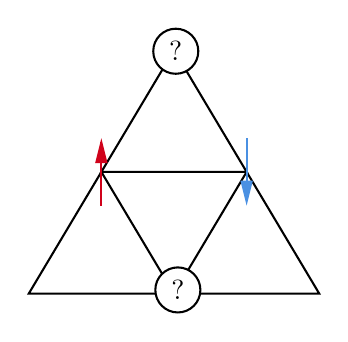
\begin{tikzpicture}[x=0.75pt,y=0.75pt,yscale=-1,xscale=1]
%uncomment if require: \path (0,300); %set diagram left start at 0, and has height of 300

%Shape: Triangle [id:dp3265971145624944] 
\draw   (225,126.33) -- (260,185) -- (190,185) -- cycle ;
%Shape: Triangle [id:dp457754747303309] 
\draw   (155,126.33) -- (190,185) -- (120,185) -- cycle ;
%Shape: Triangle [id:dp5282716496110524] 
\draw   (190,67.66) -- (225,126.33) -- (155,126.33) -- cycle ;
%Straight Lines [id:da7008008238341734] 
\draw [color={rgb, 255:red, 208; green, 2; blue, 27 }  ,draw opacity=1 ]   (155,142.56) -- (155,112.1) ;
\draw [shift={(155,110.1)}, rotate = 450] [fill={rgb, 255:red, 208; green, 2; blue, 27 }  ,fill opacity=1 ][line width=0.08]  [draw opacity=0] (12,-3) -- (0,0) -- (12,3) -- cycle    ;
%Straight Lines [id:da47122065737438956] 
\draw [color={rgb, 255:red, 74; green, 144; blue, 226 }  ,draw opacity=1 ]   (225,110.1) -- (225,140.56) ;
\draw [shift={(225,142.56)}, rotate = 270] [fill={rgb, 255:red, 74; green, 144; blue, 226 }  ,fill opacity=1 ][line width=0.08]  [draw opacity=0] (12,-3) -- (0,0) -- (12,3) -- cycle    ;
%Shape: Circle [id:dp2858034795038058] 
\draw  [fill={rgb, 255:red, 255; green, 255; blue, 255 }  ,fill opacity=1 ] (181,183.18) .. controls (181,177.19) and (185.86,172.33) .. (191.85,172.33) .. controls (197.85,172.33) and (202.71,177.19) .. (202.71,183.18) .. controls (202.71,189.18) and (197.85,194.04) .. (191.85,194.04) .. controls (185.86,194.04) and (181,189.18) .. (181,183.18) -- cycle ;

%Shape: Circle [id:dp48141040110301847] 
\draw  [fill={rgb, 255:red, 255; green, 255; blue, 255 }  ,fill opacity=1 ] (180,68.18) .. controls (180,62.19) and (184.86,57.33) .. (190.85,57.33) .. controls (196.85,57.33) and (201.71,62.19) .. (201.71,68.18) .. controls (201.71,74.18) and (196.85,79.04) .. (190.85,79.04) .. controls (184.86,79.04) and (180,74.18) .. (180,68.18) -- cycle ;


% Text Node
\draw (191.85,183.18) node   [align=left] {?};
% Text Node
\draw (190.85,68.18) node   [align=left] {?};


\end{tikzpicture}
    \caption{三角晶格上的阻挫:无法适当安排自旋方向让相邻自旋反向}
    \label{fig:triangular-frustration}
\end{figure}

\begin{info}{寻找自旋液体的尝试}{try-finding-spin-liquid}
    目前没有人找到确定无疑是自旋液体的材料。
    1973年,P.W.Anderson考虑了一个三角晶格上的反铁磁模型,来给反铁磁序的形成制造一些阻挫,因为三角晶格上显然无法形成反铁磁序(见\autoref{fig:triangular-frustration})。
    他猜测其基态为将晶格上最近邻自旋配对后将两个自旋自由度做分解
    \[
        \frac{1}{2} \otimes \frac{1}{2} = 0 \oplus 1,
    \]
    取所有可能的配对中的单态等权叠加的结果。这个状态称为\concept{RVB(Resonance Valence Bond)态}。
    如果实际上基态真的是RVB态,那么显然基态上没有形成任何磁性序,并且会有一些和磁性序上的“扰动”截然不同的激发(这些后文会详述)。
    事实证明这个说法是错误的:三角晶格上的海森堡模型的基态是一种特殊的铁磁态。虽然如此,自旋液体仍然是一个非常有趣的状态,因为,这可能是因为,对称性破缺不能发生。
    一些有机盐被认为有可能产生自旋液体,因为对它们做AMR实验观察不到任何磁性序,但始终没有定论;不少这种候选的自旋液体都被其它实验证实并非自旋液体了。
\end{info}

\section{各向同性海森堡模型中的自旋液体态}

各向同性海森堡模型是
\begin{equation}
    H = J \sum_{\pair{\vb*{i}, \vb*{j}}} \vb*{S}_{\vb*{i}} \cdot \vb*{S}_{\vb*{j}}.
    \label{eq:heisenberg-model-spin-liquid}
\end{equation}
我们没有指定晶格是什么;本节将假定此模型在某个晶格上能够形成自旋液体,并且将处理自旋液体的标准手法作用于其上。

\subsection{举例:三角晶格上的RVB态及其附近的spinon低能激发}

\subsubsection{RVB态}

我们详细说明一下\autoref{info:try-finding-spin-liquid}中的RVB态。
所谓RVB态是指这样的基态:
\begin{equation}
    \ket*{\text{ground}} \propto \sum_{\text{all possible pair partitions}} \frac{1}{\sqrt{2}} (\ket*{\uparrow \downarrow} - \ket*{\downarrow \uparrow})_{\text{pair 1}} \otimes \frac{1}{\sqrt{2}} (\ket*{\uparrow \downarrow} - \ket*{\downarrow \uparrow})_{\text{pair 2}} \otimes \cdots, 
    \label{eq:rvb-state}
\end{equation}
即我们将三角晶格划分成许多不相交的相邻自旋对,然后让每个相邻自旋对上的两个自旋处于自旋单态,即$(\ket*{\uparrow \downarrow} - \ket*{\downarrow \uparrow}) / \sqrt{2}$上,将所有可能的这种态(\autoref{fig:rvb-component}展示了一个这样的态,其中被同一块黄色区域覆盖的两个格点上的自旋处在一个自旋单态中)等权叠加起来,就得到了一个RVB态。
resonance一词来自于\eqref{eq:rvb-state}的各个组分都不是能量本征态,从而哈密顿量中,不同的自旋二聚体态之间存在跃迁,如果将一个自旋二聚体态设置为初态,那么一段时间后它会演化到另一个自旋二聚体态上,然后演化回来,如此不断振荡(如\autoref{fig:rvb-resonance}所示)。
这和“苯在两种单双键排列的构型之间振荡”的说法很相似:实际上苯分子中的电子构成离域大$\pi$键,而单双键排列的构型不是能量本征态,如果强行从单双键排列的构型出发看问题,则苯的波函数是这些构型的叠加,随着时间演化,其中各种构型的分量周期性变化。

\begin{figure}
    \centering
    \subfigure[RVB态中的一个成分]{
        

\tikzset{every picture/.style={line width=0.75pt}} %set default line width to 0.75pt        

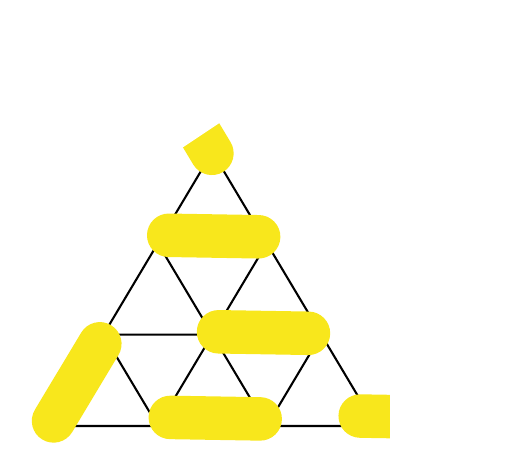
\begin{tikzpicture}[x=0.75pt,y=0.75pt,yscale=-0.75,xscale=0.75]
%uncomment if require: \path (0,300); %set diagram left start at 0, and has height of 300

%Shape: Triangle [id:dp5394198004259025] 
\draw   (272,182.33) -- (307,241) -- (237,241) -- cycle ;
%Shape: Triangle [id:dp0060243569953495335] 
\draw   (202,182.33) -- (237,241) -- (167,241) -- cycle ;
%Shape: Triangle [id:dp5009006316084215] 
\draw   (237,123.66) -- (272,182.33) -- (202,182.33) -- cycle ;
%Shape: Triangle [id:dp5954923975464252] 
\draw   (342,182.33) -- (377,241) -- (307,241) -- cycle ;
%Shape: Triangle [id:dp9717966554343387] 
\draw   (307,123.66) -- (342,182.33) -- (272,182.33) -- cycle ;
%Shape: Triangle [id:dp29175836331511373] 
\draw   (272,64.99) -- (307,123.66) -- (237,123.66) -- cycle ;
%Rounded Rect [id:dp9303927185789262] 
\draw  [draw opacity=0][fill={rgb, 255:red, 248; green, 231; blue, 28 }  ,fill opacity=1 ] (162.79,249.71) .. controls (156.17,245.74) and (154.03,237.15) .. (158,230.54) -- (187.75,181.02) .. controls (191.72,174.4) and (200.3,172.26) .. (206.92,176.24) -- (206.92,176.24) .. controls (213.53,180.21) and (215.67,188.79) .. (211.7,195.41) -- (181.96,244.92) .. controls (177.99,251.54) and (169.4,253.68) .. (162.79,249.71) -- cycle ;
%Rounded Rect [id:dp2973774835771079] 
\draw  [draw opacity=0][fill={rgb, 255:red, 248; green, 231; blue, 28 }  ,fill opacity=1 ] (230.01,118.26) .. controls (230.13,110.55) and (236.49,104.4) .. (244.21,104.52) -- (301.96,105.48) .. controls (309.68,105.61) and (315.83,111.97) .. (315.7,119.68) -- (315.7,119.68) .. controls (315.57,127.4) and (309.21,133.55) .. (301.5,133.42) -- (243.74,132.46) .. controls (236.03,132.34) and (229.88,125.98) .. (230.01,118.26) -- cycle ;
%Rounded Rect [id:dp7712557322954827] 
\draw  [draw opacity=0][fill={rgb, 255:red, 248; green, 231; blue, 28 }  ,fill opacity=1 ] (231.01,235.26) .. controls (231.13,227.55) and (237.49,221.4) .. (245.21,221.52) -- (302.96,222.48) .. controls (310.68,222.61) and (316.83,228.97) .. (316.7,236.68) -- (316.7,236.68) .. controls (316.57,244.4) and (310.21,250.55) .. (302.5,250.42) -- (244.74,249.46) .. controls (237.03,249.34) and (230.88,242.98) .. (231.01,235.26) -- cycle ;
%Rounded Rect [id:dp25009751823087134] 
\draw  [draw opacity=0][fill={rgb, 255:red, 248; green, 231; blue, 28 }  ,fill opacity=1 ] (262.01,180.26) .. controls (262.13,172.55) and (268.49,166.4) .. (276.21,166.52) -- (333.96,167.48) .. controls (341.68,167.61) and (347.83,173.97) .. (347.7,181.68) -- (347.7,181.68) .. controls (347.57,189.4) and (341.21,195.55) .. (333.5,195.42) -- (275.74,194.46) .. controls (268.03,194.34) and (261.88,187.98) .. (262.01,180.26) -- cycle ;
%Rounded Rect [id:dp12607246135910644] 
\draw  [draw opacity=0][fill={rgb, 255:red, 248; green, 231; blue, 28 }  ,fill opacity=1 ] (353.01,234.39) .. controls (353.13,226.67) and (359.49,220.52) .. (367.21,220.65) -- (424.96,221.61) .. controls (432.68,221.73) and (438.83,228.09) .. (438.7,235.81) -- (438.7,235.81) .. controls (438.57,243.52) and (432.21,249.67) .. (424.5,249.55) -- (366.74,248.59) .. controls (359.03,248.46) and (352.88,242.1) .. (353.01,234.39) -- cycle ;
%Shape: Rectangle [id:dp4625096290080499] 
\draw  [draw opacity=0][fill={rgb, 255:red, 255; green, 255; blue, 255 }  ,fill opacity=1 ] (386,214) -- (450.71,214) -- (450.71,254) -- (386,254) -- cycle ;
%Rounded Rect [id:dp22383160699593008] 
\draw  [draw opacity=0][fill={rgb, 255:red, 248; green, 231; blue, 28 }  ,fill opacity=1 ] (234.81,4.31) .. controls (241.43,0.34) and (250.01,2.49) .. (253.98,9.11) -- (283.69,58.65) .. controls (287.66,65.26) and (285.51,73.85) .. (278.89,77.81) -- (278.89,77.81) .. controls (272.27,81.78) and (263.69,79.64) .. (259.72,73.02) -- (230.02,23.48) .. controls (226.05,16.86) and (228.2,8.28) .. (234.81,4.31) -- cycle ;
%Shape: Rectangle [id:dp768095676065814] 
\draw  [draw opacity=0][fill={rgb, 255:red, 255; green, 255; blue, 255 }  ,fill opacity=1 ] (246.79,66.21) -- (207.94,7.98) -- (241.21,-14.21) -- (280.06,44.02) -- cycle ;




\end{tikzpicture}

        \label{fig:rvb-component}
    }
    \subfigure[一种低能激发态:一个自旋单态对被解开,产生两个向上的自旋]{
        

\tikzset{every picture/.style={line width=0.75pt}} %set default line width to 0.75pt        

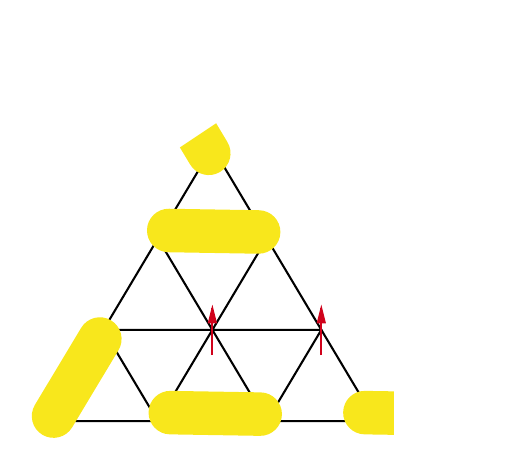
\begin{tikzpicture}[x=0.75pt,y=0.75pt,yscale=-0.75,xscale=0.75]
%uncomment if require: \path (0,300); %set diagram left start at 0, and has height of 300

%Shape: Triangle [id:dp7709012666212918] 
\draw   (292,174.46) -- (327,233.12) -- (257,233.12) -- cycle ;
%Shape: Triangle [id:dp9295040886868511] 
\draw   (222,174.46) -- (257,233.12) -- (187,233.12) -- cycle ;
%Shape: Triangle [id:dp177949788580418] 
\draw   (257,115.79) -- (292,174.46) -- (222,174.46) -- cycle ;
%Shape: Triangle [id:dp03247866415223255] 
\draw   (362,174.46) -- (397,233.12) -- (327,233.12) -- cycle ;
%Shape: Triangle [id:dp26037578632796765] 
\draw   (327,115.79) -- (362,174.46) -- (292,174.46) -- cycle ;
%Shape: Triangle [id:dp3012062348071127] 
\draw   (292,57.12) -- (327,115.79) -- (257,115.79) -- cycle ;
%Rounded Rect [id:dp4030558357818268] 
\draw  [draw opacity=0][fill={rgb, 255:red, 248; green, 231; blue, 28 }  ,fill opacity=1 ] (182.79,241.83) .. controls (176.17,237.86) and (174.03,229.28) .. (178,222.66) -- (207.75,173.14) .. controls (211.72,166.53) and (220.3,164.39) .. (226.92,168.36) -- (226.92,168.36) .. controls (233.53,172.33) and (235.67,180.92) .. (231.7,187.53) -- (201.96,237.05) .. controls (197.99,243.66) and (189.4,245.81) .. (182.79,241.83) -- cycle ;
%Rounded Rect [id:dp16737425370308645] 
\draw  [draw opacity=0][fill={rgb, 255:red, 248; green, 231; blue, 28 }  ,fill opacity=1 ] (250.01,110.39) .. controls (250.13,102.67) and (256.49,96.52) .. (264.21,96.65) -- (321.96,97.61) .. controls (329.68,97.73) and (335.83,104.09) .. (335.7,111.81) -- (335.7,111.81) .. controls (335.57,119.52) and (329.21,125.67) .. (321.5,125.55) -- (263.74,124.59) .. controls (256.03,124.46) and (249.88,118.1) .. (250.01,110.39) -- cycle ;
%Rounded Rect [id:dp7997977143532831] 
\draw  [draw opacity=0][fill={rgb, 255:red, 248; green, 231; blue, 28 }  ,fill opacity=1 ] (251.01,227.39) .. controls (251.13,219.67) and (257.49,213.52) .. (265.21,213.65) -- (322.96,214.61) .. controls (330.68,214.73) and (336.83,221.09) .. (336.7,228.81) -- (336.7,228.81) .. controls (336.57,236.52) and (330.21,242.67) .. (322.5,242.55) -- (264.74,241.59) .. controls (257.03,241.46) and (250.88,235.1) .. (251.01,227.39) -- cycle ;
%Straight Lines [id:da8204619655647556] 
\draw [color={rgb, 255:red, 208; green, 2; blue, 27 }  ,draw opacity=1 ]   (292,190.68) -- (292,160.23) ;
\draw [shift={(292,158.23)}, rotate = 450] [fill={rgb, 255:red, 208; green, 2; blue, 27 }  ,fill opacity=1 ][line width=0.08]  [draw opacity=0] (12,-3) -- (0,0) -- (12,3) -- cycle    ;
%Straight Lines [id:da301443667677862] 
\draw [color={rgb, 255:red, 208; green, 2; blue, 27 }  ,draw opacity=1 ]   (362,190.68) -- (362,160.23) ;
\draw [shift={(362,158.23)}, rotate = 450] [fill={rgb, 255:red, 208; green, 2; blue, 27 }  ,fill opacity=1 ][line width=0.08]  [draw opacity=0] (12,-3) -- (0,0) -- (12,3) -- cycle    ;
%Rounded Rect [id:dp28390331250432066] 
\draw  [draw opacity=0][fill={rgb, 255:red, 248; green, 231; blue, 28 }  ,fill opacity=1 ] (376.01,227.39) .. controls (376.13,219.67) and (382.49,213.52) .. (390.21,213.65) -- (447.96,214.61) .. controls (455.68,214.73) and (461.83,221.09) .. (461.7,228.81) -- (461.7,228.81) .. controls (461.57,236.52) and (455.21,242.67) .. (447.5,242.55) -- (389.74,241.59) .. controls (382.03,241.46) and (375.88,235.1) .. (376.01,227.39) -- cycle ;
%Shape: Rectangle [id:dp4527570591753749] 
\draw  [draw opacity=0][fill={rgb, 255:red, 255; green, 255; blue, 255 }  ,fill opacity=1 ] (409,207) -- (473.71,207) -- (473.71,247) -- (409,247) -- cycle ;
%Rounded Rect [id:dp3963770711962662] 
\draw  [draw opacity=0][fill={rgb, 255:red, 248; green, 231; blue, 28 }  ,fill opacity=1 ] (252.81,-0.47) .. controls (259.43,-4.44) and (268.01,-2.29) .. (271.98,4.32) -- (301.69,53.86) .. controls (305.66,60.48) and (303.51,69.06) .. (296.89,73.03) -- (296.89,73.03) .. controls (290.27,77) and (281.69,74.85) .. (277.72,68.23) -- (248.02,18.69) .. controls (244.05,12.08) and (246.2,3.49) .. (252.81,-0.47) -- cycle ;
%Shape: Rectangle [id:dp5531026767203489] 
\draw  [draw opacity=0][fill={rgb, 255:red, 255; green, 255; blue, 255 }  ,fill opacity=1 ] (264.79,61.43) -- (225.94,3.2) -- (259.21,-19) -- (298.06,39.23) -- cycle ;




\end{tikzpicture}

        \label{fig:rvb-up-excitation}
    }
    \caption{RVB态及其元激发}
\end{figure}

\begin{figure}
    \centering
    

\tikzset{every picture/.style={line width=0.75pt}} %set default line width to 0.75pt        

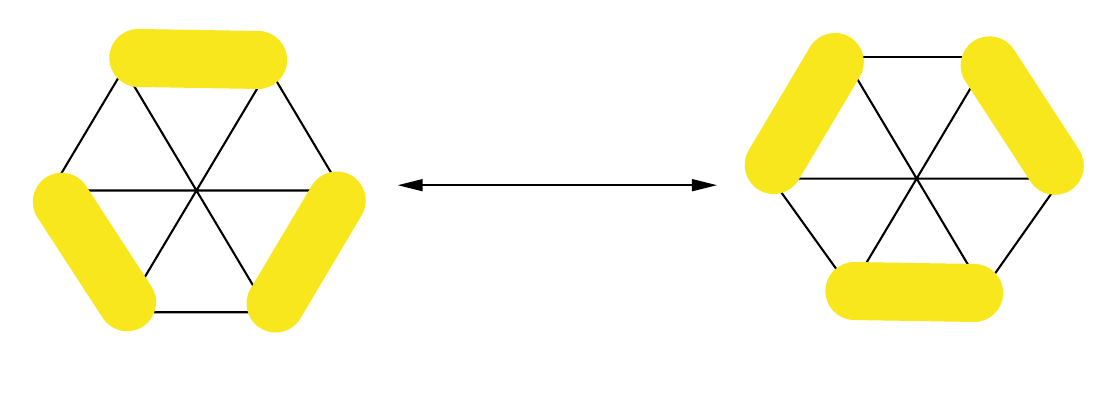
\begin{tikzpicture}[x=0.75pt,y=0.75pt,yscale=-1,xscale=1]
%uncomment if require: \path (0,300); %set diagram left start at 0, and has height of 300

%Shape: Triangle [id:dp6078109334118469] 
\draw   (162,191.55) -- (197,250.21) -- (127,250.21) -- cycle ;
%Shape: Triangle [id:dp6911272136637059] 
\draw   (127,132.88) -- (162,191.55) -- (92,191.55) -- cycle ;
%Shape: Triangle [id:dp413562090448812] 
\draw   (197,132.88) -- (232,191.55) -- (162,191.55) -- cycle ;
%Rounded Rect [id:dp956086418564118] 
\draw  [draw opacity=0][fill={rgb, 255:red, 248; green, 231; blue, 28 }  ,fill opacity=1 ] (120.01,127.48) .. controls (120.13,119.76) and (126.49,113.61) .. (134.21,113.74) -- (191.96,114.7) .. controls (199.68,114.82) and (205.83,121.18) .. (205.7,128.9) -- (205.7,128.9) .. controls (205.57,136.61) and (199.21,142.76) .. (191.5,142.64) -- (133.74,141.68) .. controls (126.03,141.55) and (119.88,135.19) .. (120.01,127.48) -- cycle ;
%Rounded Rect [id:dp28028331457934885] 
\draw  [draw opacity=0][fill={rgb, 255:red, 248; green, 231; blue, 28 }  ,fill opacity=1 ] (192.97,258.03) .. controls (186.34,254.09) and (184.15,245.52) .. (188.09,238.89) -- (217.58,189.22) .. controls (221.52,182.59) and (230.1,180.4) .. (236.73,184.34) -- (236.73,184.34) .. controls (243.37,188.28) and (245.55,196.85) .. (241.61,203.49) -- (212.12,253.15) .. controls (208.18,259.79) and (199.61,261.97) .. (192.97,258.03) -- cycle ;
%Rounded Rect [id:dp5327350177753518] 
\draw  [draw opacity=0][fill={rgb, 255:red, 248; green, 231; blue, 28 }  ,fill opacity=1 ] (89.5,185.26) .. controls (95.97,181.05) and (104.63,182.89) .. (108.83,189.36) -- (140.31,237.79) .. controls (144.51,244.26) and (142.68,252.91) .. (136.2,257.12) -- (136.2,257.12) .. controls (129.73,261.32) and (121.08,259.49) .. (116.88,253.02) -- (85.4,204.58) .. controls (81.19,198.11) and (83.03,189.46) .. (89.5,185.26) -- cycle ;

%Shape: Rectangle [id:dp7325498000306556] 
\draw  [draw opacity=0][fill={rgb, 255:red, 255; green, 255; blue, 255 }  ,fill opacity=1 ] (406,238.21) -- (470.71,238.21) -- (470.71,278.21) -- (406,278.21) -- cycle ;
%Straight Lines [id:da849412008475126] 
\draw    (439,185.81) -- (477.71,239.72) ;
%Straight Lines [id:da00812522081492606] 
\draw    (579,185.81) -- (541.71,238.72) ;
%Straight Lines [id:da9567213279891842] 
\draw    (474,127.14) -- (544,127.14) ;
%Shape: Triangle [id:dp30303117419821723] 
\draw   (509,185.81) -- (544,244.48) -- (474,244.48) -- cycle ;
%Shape: Triangle [id:dp05123361404772386] 
\draw   (474,127.14) -- (509,185.81) -- (439,185.81) -- cycle ;
%Shape: Triangle [id:dp4636941208634524] 
\draw   (544,127.14) -- (579,185.81) -- (509,185.81) -- cycle ;
%Rounded Rect [id:dp2769538449633919] 
\draw  [draw opacity=0][fill={rgb, 255:red, 248; green, 231; blue, 28 }  ,fill opacity=1 ] (465.01,239.74) .. controls (465.13,232.03) and (471.49,225.88) .. (479.21,226.01) -- (536.96,226.96) .. controls (544.68,227.09) and (550.83,233.45) .. (550.7,241.17) -- (550.7,241.17) .. controls (550.57,248.88) and (544.21,255.03) .. (536.5,254.9) -- (478.74,253.95) .. controls (471.03,253.82) and (464.88,247.46) .. (465.01,239.74) -- cycle ;
%Rounded Rect [id:dp5237290515830839] 
\draw  [draw opacity=0][fill={rgb, 255:red, 248; green, 231; blue, 28 }  ,fill opacity=1 ] (432.97,191.3) .. controls (426.34,187.36) and (424.15,178.79) .. (428.09,172.15) -- (457.58,122.49) .. controls (461.52,115.85) and (470.1,113.67) .. (476.73,117.61) -- (476.73,117.61) .. controls (483.37,121.55) and (485.55,130.12) .. (481.61,136.75) -- (452.12,186.42) .. controls (448.18,193.06) and (439.61,195.24) .. (432.97,191.3) -- cycle ;
%Rounded Rect [id:dp5382596595416931] 
\draw  [draw opacity=0][fill={rgb, 255:red, 248; green, 231; blue, 28 }  ,fill opacity=1 ] (536.5,119.52) .. controls (542.97,115.32) and (551.63,117.15) .. (555.83,123.62) -- (587.31,172.06) .. controls (591.51,178.53) and (589.68,187.18) .. (583.2,191.39) -- (583.2,191.39) .. controls (576.73,195.59) and (568.08,193.75) .. (563.88,187.28) -- (532.4,138.85) .. controls (528.19,132.38) and (530.03,123.73) .. (536.5,119.52) -- cycle ;

%Straight Lines [id:da30633418591220174] 
\draw    (261,189) -- (410.71,189) ;
\draw [shift={(412.71,189)}, rotate = 180] [fill={rgb, 255:red, 0; green, 0; blue, 0 }  ][line width=0.08]  [draw opacity=0] (12,-3) -- (0,0) -- (12,3) -- cycle    ;
\draw [shift={(259,189)}, rotate = 0] [fill={rgb, 255:red, 0; green, 0; blue, 0 }  ][line width=0.08]  [draw opacity=0] (12,-3) -- (0,0) -- (12,3) -- cycle    ;




\end{tikzpicture}

    \caption{resonance:图中的两个构型都不是能量本征态,它们可以彼此转化}
    \label{fig:rvb-resonance}
\end{figure}

现在我们分析RVB态之上的元激发。将相邻的两个自旋当成一个自由度,则它可以分解为
\begin{equation}
    \frac{1}{2} \otimes \frac{1}{2} = 0 \oplus 1,
\end{equation}
RVB态中,像\autoref{fig:rvb-component}中这样被同一块黄色区域覆盖的两个格点占据上式中的单态,那么可以给系统一个局域的激励,让某一对最近邻格点的状态变成一个自旋三重态。
\autoref{fig:rvb-up-excitation}展示了一种这样的激发态:一个$(\ket*{\uparrow \downarrow} - \ket*{\downarrow \uparrow}) / \sqrt{2}$态被激发成$\ket*{\uparrow \uparrow}$,图形化地展示就是。
组成自旋三态的两个自旋可以跑:我们总是可以重新安排自旋配对,于是我们可以认为自旋$1$的激发被拆成了两半,每一个都可以四处移动。这就得到了\concept{自旋子(spinon)}。
可以验证这是费米子,% TODO
这些自旋子全部都是自旋$1/2$的,并且总是有偶数个自旋子。

因此,至少有一类自旋系统——基态为RVB态的自旋液体——中可以演生出费米子激发,这让我们有理由相信,做费米型的部分子拆分至少对一些自旋系统是合理的。

然而,我们应当注意,\autoref{fig:rvb-up-excitation}中展示的这种自旋子元激发实际上只有在纯粹的自旋二聚体态,即一个形如\autoref{fig:rvb-component}的态上才是有明确定义的。
以RVB为基态的体系中,自旋二聚体的量子涨落现在转移到了自旋子的量子涨落上面。因此,我们需要设法用自旋算符表示出自旋子,然后代入原哈密顿量中,去得到关于自旋子的有效理论。
这里我们也可以看出为什么要构造RVB态:如果自旋二聚体态实际上接近体系的能量本征态,那么系统的低能自由度仍然是比较平凡的——我们可以将这里的spinon看成类似于XY模型中的涡旋的激发,它唯一略有不同寻常的地方就是总是成对出现。
为了让体系处在一个无法用纯经典的图像理解的量子序当中(如拓扑序中存在交换相位等等),必须引入足够的量子涨落,这会让系统基态是大量原系统的低能态的叠加,具体到自旋系统中,就是大量自旋二聚体态的叠加,这就是要构造RVB态的原因。

此处从自旋二聚体出发构造分数化的spinon的方式可以推广到其它自由度中,如可以构造粒子二聚体,一个二聚体算符为
\begin{equation}
    d_{\vb*{i} \vb*{j}} = \frac{1}{\sqrt{2}} (c^\dagger_{\vb*{i}} + c^\dagger_{\vb*{j}}),
\end{equation}
然后我们会发现在一串二聚体链的边缘格点上粒子数期望为$1/2$,从而如果一个哈密顿量的低能态都是二聚体态的话,就出现了粒子一分为二的分数化。同样,这样得到的分数化激发本身尚不具有拓扑序,但是如果有前述拉格朗日乘子引入演生规范场等机制,那么这些分数化激发将会携带规范荷,在二维情况下就会形成拓扑序,当然也可以形成其它量子序。
分数化本身和拓扑序没有直接关系(例如,AKLT链的边界态就是分数化产生的,可是其中并无拓扑序),演生规范场才是决定拓扑序行为的关键。

以上思路也可以扩展到经典的动力学理论(海森堡运动方程中取$\hbar \to 0$极限的结果,没有物理量不对易,但是有时间演化,时间演化可以看成量子涨落的残余)中:我们可以考虑流体动力学中的涡旋在纳维-斯托克斯方程中如何演化,或许还能够将流体中的一些物理量诠释成演生电磁场。
流体动力学中的涡旋有时间演化这件事的量子版本就是稳定的涡旋态是大量含有涡旋的流速场构型态的线性叠加。实际上,以流体动力学中的涡旋为粒子,流体密度可以看成磁场而流体速度可以看成电场,因此我们果真获得了演生规范场(虽然是完全经典的)!

最后,我们要大致讨论演生规范场及其物理意义。Fradkin 9.5指出了演生规范场可以从大量dimer state的线性叠加态附近得到,而dimer state需要线性组合才能够得到能量本征态本身就说明了它们有明显的量子涨落。
在\Ztwo规范理论中我们会看到是$\sigma^z$和$\sigma^x$的不对易导致了e激发和m激发的非平庸交换相位。
因此可以看到,演生规范场是量子涨落的一种体现(并且,由于Wilson loop可以任意地大而取值不变,实际上演生规范场的出现意味着系统中存在长程纠缠;通过\emph{带约束的}分数化构造演生规范场也体现了这一点)。
在二维体系中,演生规范场将导致拓扑序,我们这里构造的自旋子等是拓扑序中的任意子(或者别的有趣的量子序中的点粒子)的某种\emph{前体},它可以看成对演生规范场而言的某种“外加测试电荷”。

\begin{info}{XY模型中的拓扑序}{xy-topological-order}
    在讨论KT相变时,一个可能的疑难是,似乎经典二维XY模型中的涡旋之间也有某种弦连接,从而这里的涡旋看起来很像是$\mathbb{Z}_2$规范理论中的vison或是$\mathbb{Z}_2$荷,因此,KT相变中的有序态离拓扑序有多远?
    Sachdev在\cite{sachdev_xy}和\cite{Sachdev_2018_full}中(这个现象实际上在\cite{sedgewick2002}中已经研究过了),从一个三维的扩展的XY模型(可以看成二维的一个强关联的量子XY模型的零温路径积分,其中XY自旋可以发生各种时间演化,体现了强烈的量子涨落)出发,通过一个离散Hubbard-Stratonovich变换,引入了$\mathbb{Z}_2$规范场。注意引入Hubbard-Stratonovich变换之后,XY自旋自由度的哈密顿量将形如
    \begin{equation}
        - \sigma^z_{\vb*{i} \vb*{j}} \cos((\theta_{\vb*{i}} - \theta_{\vb*{j}}) / 2),
        \label{eq:xy-topological-order}
    \end{equation}
    其中$1/2$的因子是因为这样一来,积掉\Ztwo规范场之后得到的理论中,XY自旋自由度的哈密顿量将是
    \[
        \sim \cos^2(\theta_{\vb*{i}} - \theta_{\vb*{j}}) / 2 \sim \cos (\theta_{\vb*{i}} - \theta_{\vb*{j}}),
    \]
    正好给出引入规范场之前的XY模型。XY自旋的指向发生$2\pi$的剧变的格点连接成了一条线,其两端是两个涡旋,而由\eqref{eq:xy-topological-order},在这条线上\Ztwo规范场的$\sigma^z$自由度应该取$-1$值,否则会有很大的能量消耗。
    因此,涡旋和\Ztwo规范场中的m激发被粘合在了一起,连接XY涡旋的弦和$\sigma^z$弦被粘合在了一起,一个\Ztwo拓扑序演生出来了。

    以上推导明确地展示了XY模型中的涡旋和$\mathbb{Z}_2$规范场的vison(见\autoref{sec:gauge-charge-flux-z2})如何冻结为一个自由度,
    从而直观地展示了强关联体系如何产生演生规范场和拓扑序,以及KT相变中的涡旋和连接两个涡旋的“弦”是拓扑序中的任意子的前体、在引入强烈的量子涨落之后能够形成拓扑序这一事实,另一方面也直观地展示了二维规范场和某种粒子(在这里是KT相变中的涡旋)耦合时,规范荷如何被粘到粒子上。
\end{info}

\subsubsection{slave boson方法}

\begin{back}{自旋系统的部分子构造}{parton-spin}
    \concept{部分子方法}是指将某种自由度(如自旋自由度)写成一些费米子或是玻色子自由度(即所谓\concept{部分子})的组合,自旋算符是两个费米子或是玻色子产生湮灭算符的乘积,然后施加适当的约束来保证拆分后的物理和拆分前相同。
    这相当于说,我们使用一个费米子系统或是玻色子系统实现了一个自旋系统或是别的什么系统。
    这种方法有时也称为\concept{投影构造}。
    这样做的好处在于,如果由此得到的费米子或玻色子理论中相互作用没有强到让这些费米子和玻色子又凝聚成对,那么实际上,这意味着自旋系统演生出了类似于费米子和玻色子的激发,即拆分得到的部分子正是自旋系统的低能自由度。

    只要算符的代数关系不变,并且将部分子系统的希尔伯特空间固定为每个格点上只有一个部分子的那部分,不同的拆分方式不会改变物理。
    对自旋系统,我们手动给不同格点上的自旋算符贴上位置标签,而对费米子/玻色子系统,坐标标签是粒子产生算符自带的参数,因此表面上看起来,拆分之后得到的费米子/玻色子系统的希尔伯特空间由于对称化/反对称化的要求而受到限制,似乎部分子系统的希尔伯特空间要比自旋系统的希尔伯特空间小,但是实际上两者是同构的:自旋系统的希尔伯特空间的基形如
    \[
        \ket{\sigma_1, \sigma_2, \ldots, \sigma_n}
    \]
    而部分子系统的希尔伯特空间的基形如
    \[
        {c}^\dagger_{1 \sigma_1} {c}^\dagger_{2 \sigma_2} \cdots {c}^\dagger_{n \sigma_n} \ket{0},
    \]
    后者中交换$1, 2$等空间标签,态矢量不变或者反号,所以两种系统的希尔伯特空间是一样大的。
    不施加费米统计或是玻色统计,粒子系统的希尔伯特空间实际上要比自旋系统的希尔伯特空间大,反倒是施加了对称/反对称要求之后两者是同构的。

    不过虽然部分子构造方式不改变物理,一些拆分方式中的部分子更加接近自旋系统中实际出现的激发,从而,使用这些拆分方法得到的部分子的理论使用平均场之类的方法处理得到的结果相比于其它方案是更加可靠的。
    这和\autoref{back:gl-hubbard-stratonovich}中选择序参量很相似。

    部分子构造中的部分子如果果真能够获得足够长的寿命,则往往会是分数化现象的一种,即系统中不同的“性质”似乎被不同的激发携带着。应当注意分数化并不必然意味着拓扑序的出现:例如,Luttinger液体中就没有拓扑序。
    分数化的量子多体系统中出现拓扑序通常是因为正确的分数化方案会导致体系的希尔伯特空间扩张,为了保证物理的希尔伯特空间不变,必须向哈密顿量引入一个拉格朗日乘子以约束实际会出现的态仍然位于原有的希尔伯特空间中,这个拉格朗日乘子可能就会成为演生规范场的来源。
    更加数学地看,我们实际上是将扩张后的希尔伯特空间商掉多余的态,这有可能导致规范对称性,此时系统的低能有效理论必然是一个规范理论。
\end{back}

我们对海森堡模型使用\concept{slave boson}方法,这是指做分解
\begin{equation}
    {S}_{\vb*{i}} = \frac{1}{2} {f}_{\vb*{i} \alpha}^\dagger \vb*{\sigma}_{\alpha \beta} f_{\vb*{i} \beta},
\end{equation}
其中${f}$为费米子;每个格点上的自旋的取值由这个格点上的费米型部分子的自旋携带。
这个方法本来是用于分析携带电荷的费米子的,但是后来被用在了分析自旋上,相应的这种方法分解出来的部分子在自旋系统中就是费米子而不是玻色子。
使用费米型部分子的好处在于可以避免玻色子陷入玻色-爱因斯坦凝聚态;如果自旋系统中的元激发实际上并不处在玻色-爱因斯坦凝聚态,这就意味着我们需要某种很强的玻色型部分子之间的相互作用让玻色-爱因斯坦凝聚态不稳定,即需要很强的量子涨落,于是我们无非是把一个强关联问题转化成了另一个强关联问题。
但是,如前所述,RVB态附近的激发真的好像一个费米子,所以我们有理由相信,如果在某个晶格上海森堡模型\eqref{eq:heisenberg-model-spin-liquid}真的演生出了基态是RVB态的自旋液体,那么slave boson构造就是合理的。

slave boson拆分不是唯一的方法。还有一种拆分方式:slave fermion,即Schwinger boson。

\subsubsection{费米型spinon的探测}

中子散射实验能够激发出magnon,而magnon会“分裂”成两个spinon。因此普通的磁体做中子散射实验能够观察到清晰的峰,而以spinon为基本自由度的自旋液体就是模糊一片的,因为有两个spinon出射,从而会得到连续谱。

\subsection{spinon哈密顿量和演生$U(1)$规范场}

\subsubsection{受约束的费米子哈密顿量}

做了slave boson分解之后,哈密顿量就成为一个四阶项,描述了两个费米子的散射,写出来是
\[
    {H} = \frac{J}{4} \sum_{\pair{\vb*{i}, \vb*{j}}} (2 {f}^\dagger_{\vb*{i} \alpha} {f}_{\vb*{i} \beta} {f}_{\vb*{j} \beta}^\dagger {f}_{\vb*{j} \alpha} - {f}^\dagger_{\vb*{i} \alpha} {f}_{\vb*{i} \alpha} {f}^\dagger_{\vb*{j} \beta} {f}_{\vb*{j} \beta}),
\]
第二项由于我们要求每个格点只有单占据而可以略去,于是
\begin{equation}
    {H} = - \frac{J}{2} \sum_{\pair{\vb*{i}, \vb*{j}}} {f}_{\vb*{i} \alpha}^\dagger {f}_{\vb*{j} \beta}^\dagger {f}_{\vb*{i} \beta} {f}_{\vb*{j} \alpha}.
    \label{eq:slave-boson-hamiltonian}
\end{equation}
这个哈密顿量所在的希尔伯特空间是每个格点上有且只有一个费米子的这部分空间,写成公式就是
\begin{equation}
    f_{\vb*{i} \alpha}^\dagger f_{\vb*{j} \alpha} = 1, 
    \label{eq:one-site-one-fermion}
\end{equation}
注意其中$\vb*{i}$不求和而$\alpha$求和。
这个约束在接下来的计算中必须始终被考虑到,它的一个直接推论是
\begin{equation}
    \epsilon_{\alpha \beta} f_{\vb*{i} \alpha} f_{\vb*{i} \beta} = 0.
\end{equation}
\eqref{eq:slave-boson-hamiltonian}本身不会将一个满足\eqref{eq:one-site-one-fermion}的态转化成一个不满足这一限制的态,因此这里没有任何矛盾。

\subsubsection{路径积分和演生规范场}

下面我们使用路径积分方法引入约束\eqref{eq:one-site-one-fermion}。使用一个逐点的拉格朗日乘子$\lambda$来施加约束条件,我们有
\begin{equation}
    S[f, \bar{f}, \lambda] = \int \dd{\tau} \left( \sum_{\vb*{i}} \bar{f}_{\vb*{i} \alpha} \partial_\tau f_{\vb*{i} \alpha} + \sum_{\vb*{i}} \ii \lambda_{\vb*{i}} (\bar{f}_{\vb*{i} \alpha} f_{\vb*{i} \alpha} - 1) - \frac{J}{2} \sum_{\pair{\vb*{i}, \vb*{j}}} \bar{f}_{\vb*{i} \alpha} \bar{f}_{\vb*{j} \beta} f_{\vb*{j} \alpha} f_{\vb*{i} \beta} \right).
    \label{eq:spin-liquid-action}
\end{equation}
积掉拉格朗日乘子$\lambda_{\vb*{i}}$就能产生硬约束\eqref{eq:one-site-one-fermion}。

我们注意到,$\lambda_{\vb*{i}}$出现的位置和电势基本上一模一样(见\eqref{eq:imaginary-em-covariant-derivative}),且显然具有局域$U(1)$对称性。
这让我们猜测,\eqref{eq:spin-liquid-action}实际是一个自旋$1/2$费米子和某个$U(1)$规范场耦合的理论。
实际上,容易验证,将理论
\begin{equation}
    S[f, \bar{f}, \lambda, \chi, \bar{\chi}] = \int \dd{\tau} \left( \sum_{\vb*{i}} \bar{f}_{\vb*{i} \alpha} \partial_\tau f_{\vb*{i} \alpha} + \sum_{\vb*{i}} \ii \lambda_{\vb*{i}} (\bar{f}_{\vb*{i} \alpha} f_{\vb*{i} \alpha} - 1) + \frac{J}{2} \sum_{\pair{\vb*{i}, \vb*{j}}} (\abs{\chi_{\vb*{i} \vb*{j}}}^2 - \chi_{\vb*{i} \vb*{j}} \bar{f}_{\vb*{i} \alpha} f_{\vb*{j} \alpha} + \text{h.c.}) \right)
\end{equation}
积掉$\chi$,得到的正是\eqref{eq:spin-liquid-action}。
上式对应的哈密顿量是
\begin{equation}
    H = \frac{J}{2} \sum_{\pair{\vb*{i}, \vb*{j}}} (\abs{\chi_{\vb*{i} \vb*{j}}}^2 - \chi_{\vb*{i} \vb*{j}} {f}^\dagger_{\vb*{i} \alpha} f_{\vb*{j} \alpha} + \text{h.c.}) - \sum_{\vb*{i}} a_{0 \vb*{i}} (f^\dagger_{\vb*{i} \alpha} f_{\vb*{i} \alpha} - 1).
    \label{eq:simplest-heisenberg-u-1-hamiltonian}
\end{equation}
注意作用量中不含有$\chi$场的时间导数,从而$\chi$场没有Berry相位项;$\lambda$场也是一样,而且由于它是拉格朗日乘子,在虚时间和实时间下它的定义还需要差一个$\ii$。这里我们为了避免混乱,已经用$a_0$代替了$\lambda$。

$\chi_{\vb*{i} \vb*{j}}$看起来很像一个规范联络,不过由于它同时包含两种涨落——其振幅和相位——它实际上比规范联络稍微复杂一些。
\eqref{eq:simplest-heisenberg-u-1-hamiltonian}中存在规范对称性:做变换
\begin{equation}
    \chi_{\vb*{i} \vb*{j}} \longrightarrow \chi_{\vb*{i} \vb*{j}} \ee^{- \ii (\theta_{\vb*{i}} - \theta_{\vb*{j}})}, \quad f_{\vb*{i}} \longrightarrow \ee^{\ii \theta_{\vb*{i}}} f_{\vb*{i}},
    \label{eq:simplest-u1-gauge-heisenberg}
\end{equation}
那么哈密顿量不变。因此模型中存在演生$U(1)$规范场,并且很容易看到,这个规范场正是$\chi_{\vb*{i} \vb*{j}}$的相位。
进一步,注意到路径积分形式中,$\chi_{\vb*{i} \vb*{j}}$的振幅的涨落带来的能量变化明显比其相位发生变化带来的能量变化高(前者直接会影响$\abs{\chi_{\vb*{i} \vb*{j}}}^2$项,后者没有什么明显的影响)。
这让我们有信心认为$\abs{\chi_{\vb*{i} \vb*{j}}}$应该是一个有能隙激发而$a_{\vb*{i} \vb*{j}}$则是无能隙激发,或者至少后者比前者更低能。
简单的费曼图图形分析会说明,积掉$\chi_{\vb*{i} \vb*{j}}$能够给$a_{\vb*{i} \vb*{j}}$提供动力学,当然它也同时会产生一大堆含有$f_{\vb*{i}}$的项,如一个正比于$a_{\vb*{i} \vb*{j}}$两次方的Hubbard相互作用。
既然积掉$\chi_{\vb*{i} \vb*{j}}$后只剩下$f_{\vb*{i}}$,$a_{0 \vb*{i}}$和$a_{\vb*{i} \vb*{j}}$三种场,而$a_{0 \vb*{i}}$不参与\eqref{eq:simplest-u1-gauge-heisenberg}变换,因此,积掉$\abs{\chi_{\vb*{i} \vb*{j}}}$之后得到的有效理论中仅包含$a_{\vb*{i} \vb*{j}}$的部分是一个$U(1)$规范不变量,很明显就是$U(1)$格点规范场自身的哈密顿量,而包含$f_{\vb*{i}}$的部分则形如
\begin{equation}
    H_\text{spinon} = - \frac{J}{2} \sum_{\pair{\vb*{i}, \vb*{j}}} (\ee^{\ii a_{\vb*{i} \vb*{j}}} \bar{\chi}_{\vb*{i} \vb*{j}} {f}^\dagger_{\vb*{i} \alpha} f_{\vb*{j} \alpha} + \text{h.c.} ) - \sum_{\vb*{i}} a_{0 \vb*{i}} f^\dagger_{\vb*{i} \alpha} f_{\vb*{i} \alpha}.
    \label{eq:simplest-u1-gauge-heisenberg-spinon}
\end{equation}
总之,系统中演生出了一个$U(1)$规范场和一个费米子场,后者给出spinon,前者传递spinon之间的相互作用。

当然,总的哈密顿量肯定不止\eqref{eq:simplest-u1-gauge-heisenberg-spinon}和$U(1)$格点规范场自身的哈密顿量,例如,如前所述,还有spinon之间的正比于$a_{\vb*{i} \vb*{j}}$的Hubbard相互作用。
然而如果我们相信spinon足够接近系统的能量本征态,那么至少spinon之间不应该有强关联效应(比如说,如果Hubbard相互作用很强,那么应该有反铁磁序,然而自旋液体里面不应该有磁性序),因此,至少是定性地,\eqref{eq:simplest-u1-gauge-heisenberg-spinon}加$U(1)$格点规范场自身的哈密顿量应该构成对至少是一部分自旋液体的良好描述。

通常不计算$U(1)$格点规范理论的哈密顿量中的具体参数,因为它显而易见的困难。
原则上我们可以从平均场理论出发,通过一些方法——如大$N$展开——计算更高阶修正,但是这样非常繁琐,而仅计算有限阶可能效果也不好。

\eqref{eq:simplest-u1-gauge-heisenberg-spinon}相当于是做了一个比较“柔和”的平均场近似(忽略$\chi_{\vb*{i} \vb*{j}}$的涨落)得到的。
更为粗暴的平均场近似会直接忽略$a_{\vb*{i} \vb*{j}}$,给出自由spinon,而更加审慎的、包含了更多过程的分析则表明spinon被$U(1)$规范场粘合在一起。
\autoref{fig:two-mean-field-spin-liquid-heisenberg}图形化地展示了这一点。

\begin{figure}
    \centering
    \subfigure[最简单粗暴的平均场理论:$\abs{\chi_{\vb*{i} \vb*{j}}}$和演生规范场$a_{\vb*{i} \vb*{j}}$均被假定没有任何涨落]{
        

\tikzset{every picture/.style={line width=0.75pt}} %set default line width to 0.75pt        

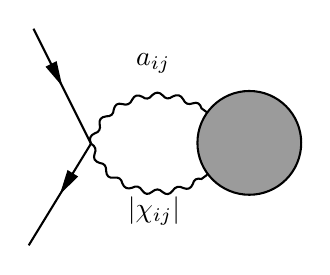
\begin{tikzpicture}[x=0.75pt,y=0.75pt,yscale=-1,xscale=1]
%uncomment if require: \path (0,300); %set diagram left start at 0, and has height of 300

%Straight Lines [id:da4145679647689646] 
\draw    (95,69) -- (122.71,124.37) ;
\draw [shift={(108.85,96.69)}, rotate = 243.42000000000002] [fill={rgb, 255:red, 0; green, 0; blue, 0 }  ][line width=0.08]  [draw opacity=0] (12,-3) -- (0,0) -- (12,3) -- cycle    ;
%Straight Lines [id:da4230340284006635] 
\draw    (122.71,124.37) -- (92.71,173.37) ;
\draw [shift={(107.71,148.87)}, rotate = 301.48] [fill={rgb, 255:red, 0; green, 0; blue, 0 }  ][line width=0.08]  [draw opacity=0] (12,-3) -- (0,0) -- (12,3) -- cycle    ;
%Shape: Circle [id:dp47035981582453945] 
\draw  [fill={rgb, 255:red, 155; green, 155; blue, 155 }  ,fill opacity=1 ] (174,124) .. controls (174,110.19) and (185.19,99) .. (199,99) .. controls (212.81,99) and (224,110.19) .. (224,124) .. controls (224,137.81) and (212.81,149) .. (199,149) .. controls (185.19,149) and (174,137.81) .. (174,124) -- cycle ;
%Curve Lines [id:da24970648369972892] 
\draw    (122.71,124.37) .. controls (121.7,122.02) and (122.28,120.38) .. (124.45,119.45) .. controls (126.62,118.85) and (127.44,117.39) .. (126.91,115.07) .. controls (126.52,112.78) and (127.56,111.5) .. (130.01,111.23) .. controls (132.37,111.27) and (133.59,110.18) .. (133.67,107.97) .. controls (134.2,105.56) and (135.58,104.67) .. (137.79,105.3) .. controls (140.04,106.04) and (141.65,105.32) .. (142.6,103.14) .. controls (143.61,101.06) and (145.22,100.61) .. (147.41,101.78) .. controls (149.19,103.16) and (150.75,102.94) .. (152.08,101.12) .. controls (153.89,99.37) and (155.59,99.36) .. (157.2,101.07) .. controls (158.61,102.87) and (160.21,103.07) .. (162.02,101.67) .. controls (164.27,100.48) and (165.98,100.92) .. (167.13,103.01) .. controls (168.06,105.14) and (169.61,105.79) .. (171.79,104.95) .. controls (173.91,104.2) and (175.3,105) .. (175.95,107.36) -- (178.71,109.37) ;
%Curve Lines [id:da3634794469098972] 
\draw    (122.71,124.37) .. controls (124.83,125.6) and (125.41,127.24) .. (124.45,129.29) .. controls (123.7,131.51) and (124.52,132.97) .. (126.91,133.68) .. controls (129.13,133.88) and (130.16,135.16) .. (130.01,137.52) .. controls (130.16,139.97) and (131.38,141.06) .. (133.67,140.78) .. controls (136,140.37) and (137.37,141.26) .. (137.79,143.44) .. controls (138.68,145.75) and (140.28,146.47) .. (142.6,145.6) .. controls (144.53,144.48) and (146.14,144.93) .. (147.41,146.96) .. controls (148.72,148.88) and (150.27,149.1) .. (152.08,147.63) .. controls (153.91,146.04) and (155.61,146.05) .. (157.2,147.68) .. controls (159.01,149.19) and (160.62,148.99) .. (162.02,147.08) .. controls (163.41,145.05) and (165.12,144.6) .. (167.13,145.73) .. controls (169.34,146.68) and (170.89,146.03) .. (171.79,143.79) .. controls (172.26,141.66) and (173.64,140.86) .. (175.95,141.39) -- (178.71,139.37) ;

% Text Node
\draw (143,79.4) node [anchor=north west][inner sep=0.75pt]    {$a_{\boldsymbol{ij}}$};
% Text Node
\draw (139,148.4) node [anchor=north west][inner sep=0.75pt]    {$|\chi _{\boldsymbol{ij}} |$};


\end{tikzpicture}

    }
    \subfigure[稍微柔和一些的平均场:假定没什么特别的物理意义的$\abs{\chi}_{\vb*{i} \vb*{j}}$没有任何涨落,但是允许$a_{\vb*{i} \vb*{j}}$有涨落]{
        

\tikzset{every picture/.style={line width=0.75pt}} %set default line width to 0.75pt        

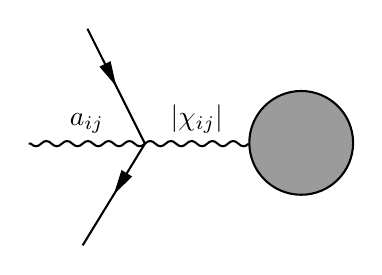
\begin{tikzpicture}[x=0.75pt,y=0.75pt,yscale=-1,xscale=1]
%uncomment if require: \path (0,300); %set diagram left start at 0, and has height of 300

%Straight Lines [id:da8963595553665786] 
\draw    (115,89) -- (142.71,144.37) ;
\draw [shift={(128.85,116.69)}, rotate = 243.42000000000002] [fill={rgb, 255:red, 0; green, 0; blue, 0 }  ][line width=0.08]  [draw opacity=0] (12,-3) -- (0,0) -- (12,3) -- cycle    ;
%Straight Lines [id:da4052777468396842] 
\draw    (142.71,144.37) -- (112.71,193.37) ;
\draw [shift={(127.71,168.87)}, rotate = 301.48] [fill={rgb, 255:red, 0; green, 0; blue, 0 }  ][line width=0.08]  [draw opacity=0] (12,-3) -- (0,0) -- (12,3) -- cycle    ;
%Shape: Circle [id:dp8961978442291645] 
\draw  [fill={rgb, 255:red, 155; green, 155; blue, 155 }  ,fill opacity=1 ] (193,144) .. controls (193,130.19) and (204.19,119) .. (218,119) .. controls (231.81,119) and (243,130.19) .. (243,144) .. controls (243,157.81) and (231.81,169) .. (218,169) .. controls (204.19,169) and (193,157.81) .. (193,144) -- cycle ;
%Straight Lines [id:da6059253418917407] 
\draw    (142.71,144.37) .. controls (144.38,142.7) and (146.04,142.7) .. (147.71,144.37) .. controls (149.38,146.04) and (151.04,146.04) .. (152.71,144.37) .. controls (154.38,142.7) and (156.04,142.7) .. (157.71,144.37) .. controls (159.38,146.04) and (161.04,146.04) .. (162.71,144.37) .. controls (164.38,142.7) and (166.04,142.7) .. (167.71,144.37) .. controls (169.38,146.04) and (171.04,146.04) .. (172.71,144.37) .. controls (174.38,142.7) and (176.04,142.7) .. (177.71,144.37) .. controls (179.38,146.04) and (181.04,146.04) .. (182.71,144.37) .. controls (184.38,142.7) and (186.04,142.7) .. (187.71,144.37) .. controls (189.38,146.04) and (191.04,146.04) .. (192.71,144.37) -- (192.71,144.37) ;
%Straight Lines [id:da7024073980693737] 
\draw    (142.71,144.37) .. controls (141.04,146.04) and (139.38,146.04) .. (137.71,144.37) .. controls (136.04,142.7) and (134.38,142.7) .. (132.71,144.37) .. controls (131.04,146.04) and (129.38,146.04) .. (127.71,144.37) .. controls (126.04,142.7) and (124.38,142.7) .. (122.71,144.37) .. controls (121.04,146.04) and (119.38,146.04) .. (117.71,144.37) .. controls (116.04,142.7) and (114.38,142.7) .. (112.71,144.37) .. controls (111.04,146.04) and (109.38,146.04) .. (107.71,144.37) .. controls (106.04,142.7) and (104.38,142.7) .. (102.71,144.37) .. controls (101.04,146.04) and (99.38,146.04) .. (97.71,144.37) .. controls (96.04,142.7) and (94.38,142.7) .. (92.71,144.37) .. controls (91.04,146.04) and (89.38,146.04) .. (87.71,144.37) -- (86.71,144.37) -- (86.71,144.37) ;

% Text Node
\draw (114.71,140.97) node [anchor=south] [inner sep=0.75pt]    {$a_{\boldsymbol{ij}}$};
% Text Node
\draw (167.71,140.97) node [anchor=south] [inner sep=0.75pt]    {$|\chi _{\boldsymbol{ij}} |$};


\end{tikzpicture}

    }
    \subfigure[相应的$a_{\vb*{i} \vb*{j}}$将要获得动力学]{
        

\tikzset{every picture/.style={line width=0.75pt}} %set default line width to 0.75pt        

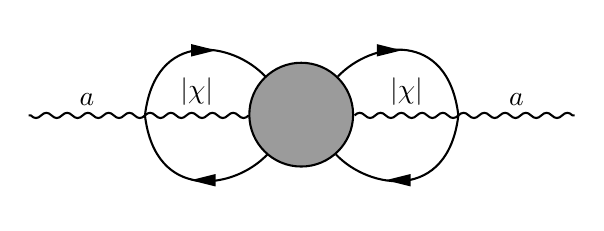
\begin{tikzpicture}[x=0.75pt,y=0.75pt,yscale=-1,xscale=1]
%uncomment if require: \path (0,300); %set diagram left start at 0, and has height of 300

%Shape: Circle [id:dp4897891030511037] 
\draw  [fill={rgb, 255:red, 155; green, 155; blue, 155 }  ,fill opacity=1 ] (213,164) .. controls (213,150.19) and (224.19,139) .. (238,139) .. controls (251.81,139) and (263,150.19) .. (263,164) .. controls (263,177.81) and (251.81,189) .. (238,189) .. controls (224.19,189) and (213,177.81) .. (213,164) -- cycle ;
%Straight Lines [id:da34822607421145757] 
\draw    (162.71,164.37) .. controls (164.38,162.7) and (166.04,162.7) .. (167.71,164.37) .. controls (169.38,166.04) and (171.04,166.04) .. (172.71,164.37) .. controls (174.38,162.7) and (176.04,162.7) .. (177.71,164.37) .. controls (179.38,166.04) and (181.04,166.04) .. (182.71,164.37) .. controls (184.38,162.7) and (186.04,162.7) .. (187.71,164.37) .. controls (189.38,166.04) and (191.04,166.04) .. (192.71,164.37) .. controls (194.38,162.7) and (196.04,162.7) .. (197.71,164.37) .. controls (199.38,166.04) and (201.04,166.04) .. (202.71,164.37) .. controls (204.38,162.7) and (206.04,162.7) .. (207.71,164.37) .. controls (209.38,166.04) and (211.04,166.04) .. (212.71,164.37) -- (212.71,164.37) ;
%Straight Lines [id:da3557842370705038] 
\draw    (162.71,164.37) .. controls (161.04,166.04) and (159.38,166.04) .. (157.71,164.37) .. controls (156.04,162.7) and (154.38,162.7) .. (152.71,164.37) .. controls (151.04,166.04) and (149.38,166.04) .. (147.71,164.37) .. controls (146.04,162.7) and (144.38,162.7) .. (142.71,164.37) .. controls (141.04,166.04) and (139.38,166.04) .. (137.71,164.37) .. controls (136.04,162.7) and (134.38,162.7) .. (132.71,164.37) .. controls (131.04,166.04) and (129.38,166.04) .. (127.71,164.37) .. controls (126.04,162.7) and (124.38,162.7) .. (122.71,164.37) .. controls (121.04,166.04) and (119.38,166.04) .. (117.71,164.37) .. controls (116.04,162.7) and (114.38,162.7) .. (112.71,164.37) .. controls (111.04,166.04) and (109.38,166.04) .. (107.71,164.37) -- (106.71,164.37) -- (106.71,164.37) ;
%Curve Lines [id:da27317319433061416] 
\draw    (162.71,164.37) .. controls (167.71,122.6) and (204.71,128.6) .. (220.71,145.6) ;
%Curve Lines [id:da5398727256974714] 
\draw    (162.71,164.37) .. controls (167.71,206.15) and (205.71,200.15) .. (221.71,183.15) ;
%Straight Lines [id:da712060576823661] 
\draw    (197,133) ;
\draw [shift={(197,133)}, rotate = 180] [fill={rgb, 255:red, 0; green, 0; blue, 0 }  ][line width=0.08]  [draw opacity=0] (12,-3) -- (0,0) -- (12,3) -- cycle    ;
%Straight Lines [id:da22975001009365803] 
\draw    (191.71,195.6) -- (186.71,195.6) ;
\draw [shift={(184.71,195.6)}, rotate = 360] [fill={rgb, 255:red, 0; green, 0; blue, 0 }  ][line width=0.08]  [draw opacity=0] (12,-3) -- (0,0) -- (12,3) -- cycle    ;
%Straight Lines [id:da8103108566723722] 
\draw    (313.71,164.37) .. controls (312.04,166.04) and (310.38,166.04) .. (308.71,164.37) .. controls (307.04,162.7) and (305.38,162.7) .. (303.71,164.37) .. controls (302.04,166.04) and (300.38,166.04) .. (298.71,164.37) .. controls (297.04,162.7) and (295.38,162.7) .. (293.71,164.37) .. controls (292.04,166.04) and (290.38,166.04) .. (288.71,164.37) .. controls (287.04,162.7) and (285.38,162.7) .. (283.71,164.37) .. controls (282.04,166.04) and (280.38,166.04) .. (278.71,164.37) .. controls (277.04,162.7) and (275.38,162.7) .. (273.71,164.37) .. controls (272.04,166.04) and (270.38,166.04) .. (268.71,164.37) .. controls (267.04,162.7) and (265.38,162.7) .. (263.71,164.37) -- (263.71,164.37) ;
%Straight Lines [id:da8909548026759186] 
\draw    (313.71,164.37) .. controls (315.38,162.7) and (317.04,162.7) .. (318.71,164.37) .. controls (320.38,166.04) and (322.04,166.04) .. (323.71,164.37) .. controls (325.38,162.7) and (327.04,162.7) .. (328.71,164.37) .. controls (330.38,166.04) and (332.04,166.04) .. (333.71,164.37) .. controls (335.38,162.7) and (337.04,162.7) .. (338.71,164.37) .. controls (340.38,166.04) and (342.04,166.04) .. (343.71,164.37) .. controls (345.38,162.7) and (347.04,162.7) .. (348.71,164.37) .. controls (350.38,166.04) and (352.04,166.04) .. (353.71,164.37) .. controls (355.38,162.7) and (357.04,162.7) .. (358.71,164.37) .. controls (360.38,166.04) and (362.04,166.04) .. (363.71,164.37) .. controls (365.38,162.7) and (367.04,162.7) .. (368.71,164.37) -- (369.71,164.37) -- (369.71,164.37) ;
%Curve Lines [id:da08747461298796533] 
\draw    (313.71,164.37) .. controls (308.71,122.6) and (271.71,128.6) .. (255.71,145.6) ;
%Curve Lines [id:da04052245252925668] 
\draw    (313.71,164.37) .. controls (308.71,206.15) and (270.71,200.15) .. (254.71,183.15) ;
%Straight Lines [id:da12788429694428705] 
\draw    (286.41,133) ;
\draw [shift={(286.41,133)}, rotate = 180] [fill={rgb, 255:red, 0; green, 0; blue, 0 }  ][line width=0.08]  [draw opacity=0] (12,-3) -- (0,0) -- (12,3) -- cycle    ;
%Straight Lines [id:da809020774422768] 
\draw    (285.71,195.6) -- (280.71,195.6) ;
\draw [shift={(278.71,195.6)}, rotate = 360] [fill={rgb, 255:red, 0; green, 0; blue, 0 }  ][line width=0.08]  [draw opacity=0] (12,-3) -- (0,0) -- (12,3) -- cycle    ;

% Text Node
\draw (134.71,160.97) node [anchor=south] [inner sep=0.75pt]    {$a$};
% Text Node
\draw (187.71,160.97) node [anchor=south] [inner sep=0.75pt]    {$|\chi |$};
% Text Node
\draw (341.71,160.97) node [anchor=south] [inner sep=0.75pt]    {$a$};
% Text Node
\draw (288.71,160.97) node [anchor=south] [inner sep=0.75pt]    {$|\chi |$};


\end{tikzpicture}

    }
    \caption{两种平均场理论的对比}
    \label{fig:two-mean-field-spin-liquid-heisenberg}
\end{figure}

\subsubsection{$U(1)$演生规范场是否真的存在?}

不同格点的基本自由度彼此对易的海森堡模型中有费米型spinon本身已经很离谱了,现在还多出来一个$U(1)$格点规范场。
由于我们并不知道受到阻挫的海森堡模型的基态到底是什么,因此实际上也无从推测在其附近能够有费米型spinon和演生规范场$a_{\vb*{i} \vb*{j}}$,而$\abs{\chi_{\vb*{i} \vb*{j}}}$的涨落受到压制的平均场基态是否真的和阻挫海森堡模型的基态足够接近。
如果两者并不十分接近,通过以上平均场方法得到的“低能有效理论”\eqref{eq:simplest-u1-gauge-heisenberg-spinon}就是假象了。

我们知道规范理论有禁闭相,在其中规范场牢牢地将与之耦合的粒子固定在一起,从而系统的低能自由度中没有规范场也没有与之耦合的粒子,因为两者的能隙都非常大。QCD在低能标下就是这样。
对海森堡模型,如果\eqref{eq:simplest-u1-gauge-heisenberg-spinon}耦合上$U(1)$规范场后处于禁闭相,那么就没有低能的spinon——这正好说明系统中只存在\emph{玻色型}的自旋涨落,如自旋波一类。海森堡模型没有形成spinon时就是这样的。
因此此时演生规范理论\eqref{eq:simplest-u1-gauge-heisenberg-spinon}是无用的,但是\emph{不是错的}——我们从它出发得到了合乎常理的结论,虽然绕了一个大弯子。

另一方面,对于自旋液体态,做完slave boson分解后直接对spinon做平均场是有问题的,因为我们手动地破缺了每个格点上粒子数始终唯一的限制,但是实际上,由于这个费米子模型实际上是一个自旋模型,这样的破缺是不正确的。
为此在路径积分表述中,我们加入一个拉格朗日乘子项来固定每个格点上的粒子数,具体的拉格朗日乘子大小不能确定,是路径积分中需要额外做积分的一个场变量。
在正则量子化表述中可以通过将一个投影算符作用在普通的平均场波函数上来得到更加接近实际情况的波函数。
% TODO, 以及 Fradkin 9.5显式地说明了可以从dimer model出发得到规范场

我们很关心演生规范场是不是禁闭的,如果是的话,它将不会有任何物理效应,因为低能下规范场将会非常强,从而spinon被紧密结合在一起,不会出现任何spinon涨落(而如果能量足够高,那就不再能够“只考虑基态附近的涨落”,而且,在凝聚态物理的语境下,能量足够高通常意味着温度足够高,而热涨落足以破坏大量有趣的量子纠缠)。
这种情况下不存在独立的spinon激发以及规范场涨落,也就没有自旋液体态。

\subsection{演生$SU(2)$规范场}

如果\eqref{eq:spin-liquid-action}有非平庸的鞍点解,它附近的涨落肯定会破坏一些局域$U(1)$对称性。
现在我们假定在某些情况下可以有这样的鞍点解:$\Delta_{\vb*{i} \vb*{j}}$非零,但是$\chi_{\vb*{i} \vb*{j}}$为零。
此时
\begin{equation}
    S = \int_0^\beta \dd{\tau} \left( \sum_{\vb*{i}} \bar{f}_{\vb*{i} \alpha} (\partial_\tau - \ii \lambda_{\vb*{i}}) f_{\vb*{i} \alpha} - \tilde{J} \sum_{\pair{\vb*{i}, \vb*{j}}} \bar{\Delta}_{\vb*{i} \vb*{j}} \epsilon_{\alpha \beta} b_{\vb*{i} \alpha} b_{\vb*{j} \beta} + \text{h.c.} \right)
\end{equation}

设
\begin{equation}
    {\Delta}_{\vb*{i} \vb*{j}} = \epsilon_{\alpha \beta} {f}_{\vb*{i} \alpha} {f}_{\vb*{j} \beta}, \quad {\chi} = {f}^\dagger_{\vb*{i} \alpha} {f}_{\vb*{j} \alpha},
\end{equation}
有
\begin{equation}
    {H} = - \frac{J}{2} \sum_{\pair{\vb*{i}, \vb*{j}}} {\Delta}^\dagger_{\vb*{i} \vb*{j}} {\Delta}_{\vb*{i} \vb*{j}} = - \frac{J}{2} \sum_{\pair{\vb*{i}, \vb*{j}}} {\chi}_{\vb*{i} \vb*{j}}^\dagger {\chi}_{\vb*{i} \vb*{j}} = - \frac{J}{4} \sum_{\pair{\vb*{i}, \vb*{j}}} ({\Delta}^\dagger_{\vb*{i} \vb*{j}} {\Delta}_{\vb*{i} \vb*{j}} + {\chi}^\dagger_{\vb*{i} \vb*{j}} {\chi}_{\vb*{i} \vb*{j}}),
\end{equation}
于是可以对最后一个形式做平均场近似;我们引入了两个参量,为了增加变分计算的参数,使之更加有效。
直接做平均场分解,有(我们将算符的期望值去掉帽子)
\[
    {H}_\text{MF} = - \frac{J}{4} \sum_{\pair{\vb*{i}, \vb*{j}}} (\Delta_{\vb*{i} \vb*{j}}^* {\Delta}_{\vb*{i} \vb*{j}} + {\Delta}_{\vb*{i} \vb*{j}} \Delta_{\vb*{i} \vb*{j}} - \abs*{\Delta_{\vb*{i} \vb*{j}}}^2) - \frac{J}{4} \sum_{\pair{\vb*{i}, \vb*{j}}} (\chi_{\vb*{i} \vb*{j}}^* {\chi}_{\vb*{i} \vb*{j}} + {\chi}_{\vb*{i} \vb*{j}} \chi_{\vb*{i} \vb*{j}} - \abs*{\chi_{\vb*{i} \vb*{j}}}^2).
\]
但是,实际上应该将系数设置成$3/8$,因为数值计算说明,直接做平均场近似效果非常糟糕。我们下面将会将系数统一称为$\tilde{J}$。
实际上严格计算平均场理论并没有什么意义,因为平均场理论的定量结果向来是非常糟糕的,而使用变分蒙特卡洛方法不难得到较为精确的结果。

参考: 
RMP 51, 657, 1979
RMP 78 17 2006

flux-fusion anomaly test

LSM theorem: if in each unit cell of a system there are odd spin-$1/2$, there must be ground state degeneracy.

所以我们现在看到,磁体的相实际上是非常多样的,包括
\begin{enumerate}
    \item 平凡的顺磁相,没有基态简并。
    \item 对称性自发破缺相,存在基态简并。
    \item 拓扑序带来的基态简并。
    \item 无能隙激发带来的基态简并。
\end{enumerate}

\section{自旋液体模型的分类}

我们可以看到,要想确定一个给定的自旋模型中有没有解禁闭的自旋液体是非常难以判断的:我们得到自旋液体的低能有效理论的过程——对自旋自由度做一定的部分子构造,获得spinon,通过对希尔伯特空间的限制引入$\chi_{\vb*{i} \vb*{j}}$场,发现规范结构,于是最终写出spinon和演生规范场耦合的有效理论——实际上并没有用到太多关于原理论的信息。
例如,实际上从来没有人计算过演生规范场中的各种系数,自然也无法确定一个给定的自旋模型的演生规范场是禁闭的还是解禁闭的,从而也不知道它是否能够给出解禁闭的自旋液体态。

这意味着实际上研究自旋液体更好的办法是反过来:写下一个某种物质场和规范场耦合的理论,并要求该理论的禁闭相是一个自旋模型,我们就能够研究所有的自旋液体,虽然我们并不知道它们如何能够被演生出来。
实际上,我们在研究寻常的能带电子态时使用的是一模一样的方法:我们只是假定相互作用较弱,从而只是修正了一下能带结构而已。
能带电子态和自旋液体态的不同在于能带论中的参数可以被第一性原理地计算(如\autoref{chap:dft}),但是自旋液体态——以及大部分强关联物态——中的各种参数不能被第一性原理地计算。

在二维自旋液体中如果出现了演生规范场,那么一般就意味着出现了拓扑序,因为规范场可以产生非平凡的Berry相位(见\autoref{back:anyon-field-theory})。
这是寻找自旋液体的一个重要动机:它给出了产生分数量子霍尔效应以外的拓扑序的方法。

\subsection{自旋液体中的对称性分数化}

大部分对称性都有所谓的对称性反常,需要生存在高维SPT(??)的边界态上。
直接从对称性分析出发可以得到大量的态,但是满足一定非常合理的条件的态是很少的,这些态均可以直接使用平均场构造出来。

\section{Toric-code模型}

\subsection{Toric-code哈密顿量与解析解}

Kitaev最早提出了一种模型,作为一种可能的量子计算纠错编码,他发现这个模型放在一个环面上可以有非常有趣的结果。
然而,事后发现这个模型实际上展现出了一个拓扑序。
这个模型是一个严格可解模型,同时又是一个自旋液体(其基本自由度是自旋,并且没有磁性序),因此值得在这里深入研究。

\begin{figure}
    \centering
    \subfigure[Toric-code模型的希尔伯特空间的一组基底由这样的态构成:每条边上都或是有确定的$\sigma^z$或是有确定的$\sigma^x$]{
        

\tikzset{every picture/.style={line width=0.75pt}} %set default line width to 0.75pt        

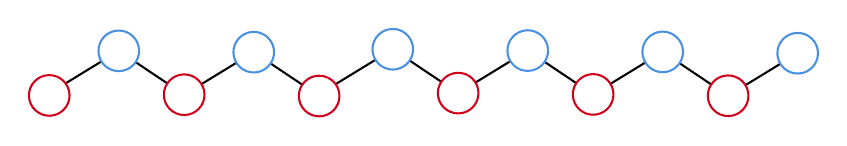
\begin{tikzpicture}[x=0.75pt,y=0.75pt,yscale=-1,xscale=1]
%uncomment if require: \path (0,300); %set diagram left start at 0, and has height of 300

%Straight Lines [id:da5978907907830429] 
\draw    (101.11,108.45) -- (132.62,129.57) ;
%Straight Lines [id:da6479636898097754] 
\draw    (166.14,109.09) -- (197.65,130.21) ;
%Straight Lines [id:da20799022198939388] 
\draw    (233.12,107.68) -- (264.64,128.81) ;
%Straight Lines [id:da7588059918995707] 
\draw    (298.15,108.32) -- (329.66,129.45) ;
%Straight Lines [id:da04554146426034689] 
\draw    (363.18,108.96) -- (394.69,130.09) ;
%Straight Lines [id:da6866628962323054] 
\draw    (67.6,128.94) -- (101.11,108.45) ;
%Shape: Circle [id:dp960424577904551] 
\draw  [color={rgb, 255:red, 208; green, 2; blue, 27 }  ,draw opacity=1 ][fill={rgb, 255:red, 255; green, 255; blue, 255 }  ,fill opacity=1 ] (57.83,130.14) .. controls (57.72,124.74) and (62.01,120.27) .. (67.41,120.15) .. controls (72.82,120.04) and (77.29,124.33) .. (77.4,129.73) .. controls (77.51,135.13) and (73.23,139.61) .. (67.82,139.72) .. controls (62.42,139.83) and (57.95,135.54) .. (57.83,130.14) -- cycle ;
%Shape: Circle [id:dp278517736754311] 
\draw  [color={rgb, 255:red, 74; green, 144; blue, 226 }  ,draw opacity=1 ][fill={rgb, 255:red, 255; green, 255; blue, 255 }  ,fill opacity=1 ] (91.32,108.65) .. controls (91.21,103.25) and (95.5,98.78) .. (100.9,98.67) .. controls (106.31,98.55) and (110.78,102.84) .. (110.89,108.24) .. controls (111.01,113.65) and (106.72,118.12) .. (101.31,118.23) .. controls (95.91,118.35) and (91.44,114.06) .. (91.32,108.65) -- cycle ;
%Straight Lines [id:da8951114155214333] 
\draw    (132.62,129.57) -- (166.14,109.09) ;
%Shape: Circle [id:dp6119193772576137] 
\draw  [color={rgb, 255:red, 208; green, 2; blue, 27 }  ,draw opacity=1 ][fill={rgb, 255:red, 255; green, 255; blue, 255 }  ,fill opacity=1 ] (122.84,129.78) .. controls (122.73,124.38) and (127.02,119.9) .. (132.42,119.79) .. controls (137.82,119.68) and (142.29,123.97) .. (142.41,129.37) .. controls (142.52,134.77) and (138.23,139.25) .. (132.83,139.36) .. controls (127.43,139.47) and (122.95,135.18) .. (122.84,129.78) -- cycle ;
%Shape: Circle [id:dp7508217961101133] 
\draw  [color={rgb, 255:red, 74; green, 144; blue, 226 }  ,draw opacity=1 ][fill={rgb, 255:red, 255; green, 255; blue, 255 }  ,fill opacity=1 ] (156.35,109.29) .. controls (156.24,103.89) and (160.53,99.42) .. (165.93,99.3) .. controls (171.33,99.19) and (175.81,103.48) .. (175.92,108.88) .. controls (176.03,114.29) and (171.74,118.76) .. (166.34,118.87) .. controls (160.94,118.98) and (156.47,114.7) .. (156.35,109.29) -- cycle ;
%Straight Lines [id:da6824105788244417] 
\draw    (199.61,128.17) -- (233.12,107.68) ;
%Shape: Circle [id:dp6550057353578134] 
\draw  [color={rgb, 255:red, 208; green, 2; blue, 27 }  ,draw opacity=1 ][fill={rgb, 255:red, 255; green, 255; blue, 255 }  ,fill opacity=1 ] (187.87,130.42) .. controls (187.75,125.01) and (192.04,120.54) .. (197.45,120.43) .. controls (202.85,120.32) and (207.32,124.6) .. (207.43,130.01) .. controls (207.55,135.41) and (203.26,139.88) .. (197.86,140) .. controls (192.45,140.11) and (187.98,135.82) .. (187.87,130.42) -- cycle ;
%Shape: Circle [id:dp2789113887024053] 
\draw  [color={rgb, 255:red, 74; green, 144; blue, 226 }  ,draw opacity=1 ][fill={rgb, 255:red, 255; green, 255; blue, 255 }  ,fill opacity=1 ] (223.34,107.89) .. controls (223.22,102.49) and (227.51,98.01) .. (232.92,97.9) .. controls (238.32,97.79) and (242.79,102.08) .. (242.9,107.48) .. controls (243.02,112.88) and (238.73,117.35) .. (233.33,117.47) .. controls (227.92,117.58) and (223.45,113.29) .. (223.34,107.89) -- cycle ;
%Straight Lines [id:da9835803759861903] 
\draw [color={rgb, 255:red, 0; green, 0; blue, 0 }  ,draw opacity=1 ][fill={rgb, 255:red, 208; green, 2; blue, 27 }  ,fill opacity=1 ]   (264.64,128.81) -- (298.15,108.32) ;
%Shape: Circle [id:dp3465061446468005] 
\draw  [color={rgb, 255:red, 208; green, 2; blue, 27 }  ,draw opacity=1 ][fill={rgb, 255:red, 255; green, 255; blue, 255 }  ,fill opacity=1 ] (254.85,129.02) .. controls (254.74,123.61) and (259.03,119.14) .. (264.43,119.03) .. controls (269.83,118.91) and (274.31,123.2) .. (274.42,128.61) .. controls (274.53,134.01) and (270.24,138.48) .. (264.84,138.59) .. controls (259.44,138.71) and (254.97,134.42) .. (254.85,129.02) -- cycle ;
%Shape: Circle [id:dp2919589177523425] 
\draw  [color={rgb, 255:red, 74; green, 144; blue, 226 }  ,draw opacity=1 ][fill={rgb, 255:red, 255; green, 255; blue, 255 }  ,fill opacity=1 ] (288.36,108.53) .. controls (288.25,103.12) and (292.54,98.65) .. (297.94,98.54) .. controls (303.35,98.43) and (307.82,102.71) .. (307.93,108.12) .. controls (308.05,113.52) and (303.76,117.99) .. (298.35,118.11) .. controls (292.95,118.22) and (288.48,113.93) .. (288.36,108.53) -- cycle ;
%Straight Lines [id:da3388603264007448] 
\draw    (329.66,129.45) -- (363.18,108.96) ;
%Shape: Circle [id:dp22822608286568746] 
\draw  [color={rgb, 255:red, 208; green, 2; blue, 27 }  ,draw opacity=1 ][fill={rgb, 255:red, 255; green, 255; blue, 255 }  ,fill opacity=1 ] (319.88,129.65) .. controls (319.77,124.25) and (324.06,119.78) .. (329.46,119.66) .. controls (334.86,119.55) and (339.33,123.84) .. (339.45,129.24) .. controls (339.56,134.65) and (335.27,139.12) .. (329.87,139.23) .. controls (324.47,139.35) and (319.99,135.06) .. (319.88,129.65) -- cycle ;
%Shape: Circle [id:dp9731435281234146] 
\draw  [color={rgb, 255:red, 74; green, 144; blue, 226 }  ,draw opacity=1 ][fill={rgb, 255:red, 255; green, 255; blue, 255 }  ,fill opacity=1 ] (353.39,109.17) .. controls (353.28,103.76) and (357.57,99.29) .. (362.97,99.18) .. controls (368.37,99.06) and (372.85,103.35) .. (372.96,108.76) .. controls (373.07,114.16) and (368.78,118.63) .. (363.38,118.74) .. controls (357.98,118.86) and (353.51,114.57) .. (353.39,109.17) -- cycle ;
%Straight Lines [id:da7953208412330044] 
\draw    (394.69,130.09) -- (428.2,109.6) ;
%Shape: Circle [id:dp6293699664956078] 
\draw  [color={rgb, 255:red, 208; green, 2; blue, 27 }  ,draw opacity=1 ][fill={rgb, 255:red, 255; green, 255; blue, 255 }  ,fill opacity=1 ] (384.91,130.29) .. controls (384.79,124.89) and (389.08,120.42) .. (394.49,120.3) .. controls (399.89,120.19) and (404.36,124.48) .. (404.48,129.88) .. controls (404.59,135.29) and (400.3,139.76) .. (394.9,139.87) .. controls (389.49,139.98) and (385.02,135.7) .. (384.91,130.29) -- cycle ;
%Shape: Circle [id:dp5339722494647174] 
\draw  [color={rgb, 255:red, 74; green, 144; blue, 226 }  ,draw opacity=1 ][fill={rgb, 255:red, 255; green, 255; blue, 255 }  ,fill opacity=1 ] (418.42,109.8) .. controls (418.31,104.4) and (422.6,99.93) .. (428,99.82) .. controls (433.4,99.7) and (437.87,103.99) .. (437.99,109.39) .. controls (438.1,114.8) and (433.81,119.27) .. (428.41,119.38) .. controls (423.01,119.5) and (418.53,115.21) .. (418.42,109.8) -- cycle ;




\end{tikzpicture}

    }
    \subfigure[$A$激发定义在格点上,上图是一个$A$激发的例子]{
        

\tikzset{every picture/.style={line width=0.75pt}} %set default line width to 0.75pt        

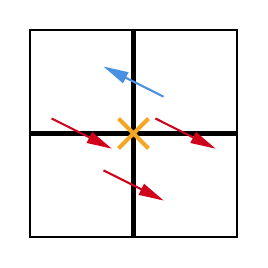
\begin{tikzpicture}[x=0.75pt,y=0.75pt,yscale=-1,xscale=1]
%uncomment if require: \path (0,300); %set diagram left start at 0, and has height of 300

%Shape: Square [id:dp6654025093743159] 
\draw   (140,67) -- (190,67) -- (190,117) -- (140,117) -- cycle ;
%Shape: Square [id:dp6286524465515233] 
\draw   (190,67) -- (240,67) -- (240,117) -- (190,117) -- cycle ;
%Shape: Square [id:dp6519468109347835] 
\draw   (140,117) -- (190,117) -- (190,167) -- (140,167) -- cycle ;
%Shape: Square [id:dp2265935355822739] 
\draw   (190,117) -- (240,117) -- (240,167) -- (190,167) -- cycle ;
%Straight Lines [id:da21658691245720751] 
\draw [line width=1.5]    (190,67) -- (190,117) ;
%Straight Lines [id:da3177017321913107] 
\draw [line width=1.5]    (140,117) -- (190,117) ;
%Straight Lines [id:da01915738195349781] 
\draw [line width=1.5]    (190,117) -- (190,167) ;
%Straight Lines [id:da717616113838583] 
\draw [line width=1.5]    (190,117) -- (240,117) ;
%Straight Lines [id:da8258680195288246] 
\draw [color={rgb, 255:red, 245; green, 166; blue, 35 }  ,draw opacity=1 ][line width=1.5]    (190,117) ;
\draw [shift={(190,117)}, rotate = 45] [color={rgb, 255:red, 245; green, 166; blue, 35 }  ,draw opacity=1 ][line width=1.5]    (-10.17,0) -- (10.17,0)(0,10.17) -- (0,-10.17)   ;
%Straight Lines [id:da10440190731652677] 
\draw [color={rgb, 255:red, 208; green, 2; blue, 27 }  ,draw opacity=1 ]   (200.54,109.75) -- (227.67,123.35) ;
\draw [shift={(229.46,124.25)}, rotate = 206.63] [fill={rgb, 255:red, 208; green, 2; blue, 27 }  ,fill opacity=1 ][line width=0.08]  [draw opacity=0] (12,-3) -- (0,0) -- (12,3) -- cycle    ;
%Straight Lines [id:da6468653685487751] 
\draw [color={rgb, 255:red, 74; green, 144; blue, 226 }  ,draw opacity=1 ]   (204.46,99.25) -- (177.33,85.65) ;
\draw [shift={(175.54,84.75)}, rotate = 386.63] [fill={rgb, 255:red, 74; green, 144; blue, 226 }  ,fill opacity=1 ][line width=0.08]  [draw opacity=0] (12,-3) -- (0,0) -- (12,3) -- cycle    ;
%Straight Lines [id:da7493786508982636] 
\draw [color={rgb, 255:red, 208; green, 2; blue, 27 }  ,draw opacity=1 ]   (175.54,134.75) -- (202.67,148.35) ;
\draw [shift={(204.46,149.25)}, rotate = 206.63] [fill={rgb, 255:red, 208; green, 2; blue, 27 }  ,fill opacity=1 ][line width=0.08]  [draw opacity=0] (12,-3) -- (0,0) -- (12,3) -- cycle    ;
%Straight Lines [id:da32966501733867193] 
\draw [color={rgb, 255:red, 208; green, 2; blue, 27 }  ,draw opacity=1 ]   (150.54,109.75) -- (177.67,123.35) ;
\draw [shift={(179.46,124.25)}, rotate = 206.63] [fill={rgb, 255:red, 208; green, 2; blue, 27 }  ,fill opacity=1 ][line width=0.08]  [draw opacity=0] (12,-3) -- (0,0) -- (12,3) -- cycle    ;




\end{tikzpicture}
      
    }
    \vfill
    \subfigure[$B$激发定义在正方形方块上,上图是一个$B$激发的例子]{
        

\tikzset{every picture/.style={line width=0.75pt}} %set default line width to 0.75pt        

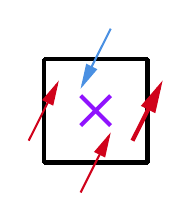
\begin{tikzpicture}[x=0.75pt,y=0.75pt,yscale=-1,xscale=1]
%uncomment if require: \path (0,300); %set diagram left start at 0, and has height of 300

%Shape: Square [id:dp06008287812795965] 
\draw   (192,54) -- (242,54) -- (242,104) -- (192,104) -- cycle ;
%Straight Lines [id:da5345790011660227] 
\draw [line width=1.5]    (192,54) -- (192,104) ;
%Straight Lines [id:da8934908293124699] 
\draw [line width=1.5]    (242,54) -- (242,104) ;
%Straight Lines [id:da6163816696768483] 
\draw [line width=1.5]    (192,54) -- (242,54) ;
%Straight Lines [id:da13968764975578463] 
\draw [line width=1.5]    (192,104) -- (242,104) ;
%Straight Lines [id:da6360739318940407] 
\draw [color={rgb, 255:red, 208; green, 2; blue, 27 }  ,draw opacity=1 ]   (184.75,93.46) -- (198.35,66.33) ;
\draw [shift={(199.25,64.54)}, rotate = 476.63] [fill={rgb, 255:red, 208; green, 2; blue, 27 }  ,fill opacity=1 ][line width=0.08]  [draw opacity=0] (12,-3) -- (0,0) -- (12,3) -- cycle    ;
%Straight Lines [id:da2436020984695373] 
\draw [color={rgb, 255:red, 74; green, 144; blue, 226 }  ,draw opacity=1 ]   (224.25,39.54) -- (210.65,66.67) ;
\draw [shift={(209.75,68.46)}, rotate = 296.63] [fill={rgb, 255:red, 74; green, 144; blue, 226 }  ,fill opacity=1 ][line width=0.08]  [draw opacity=0] (12,-3) -- (0,0) -- (12,3) -- cycle    ;
%Straight Lines [id:da6361964039179109] 
\draw [color={rgb, 255:red, 208; green, 2; blue, 27 }  ,draw opacity=1 ][line width=1.5]    (234.75,93.46) -- (247.46,68.12) ;
\draw [shift={(249.25,64.54)}, rotate = 476.63] [fill={rgb, 255:red, 208; green, 2; blue, 27 }  ,fill opacity=1 ][line width=0.08]  [draw opacity=0] (15.6,-3.9) -- (0,0) -- (15.6,3.9) -- cycle    ;
%Straight Lines [id:da7397146382660318] 
\draw [color={rgb, 255:red, 208; green, 2; blue, 27 }  ,draw opacity=1 ]   (209.75,118.46) -- (223.35,91.33) ;
\draw [shift={(224.25,89.54)}, rotate = 476.63] [fill={rgb, 255:red, 208; green, 2; blue, 27 }  ,fill opacity=1 ][line width=0.08]  [draw opacity=0] (12,-3) -- (0,0) -- (12,3) -- cycle    ;
%Straight Lines [id:da059453193677352134] 
\draw [color={rgb, 255:red, 144; green, 19; blue, 254 }  ,draw opacity=1 ][line width=1.5]    (217,79) ;
\draw [shift={(217,79)}, rotate = 45] [color={rgb, 255:red, 144; green, 19; blue, 254 }  ,draw opacity=1 ][line width=1.5]    (-10.17,0) -- (10.17,0)(0,10.17) -- (0,-10.17)   ;




\end{tikzpicture}
    }
    \subfigure[虽然$\sigma^x$和$\sigma^z$之间有量子涨落,但是$A$和$B$对易,从而系统的能量本征态可以用$A$激发和$B$激发标记;通过数自由度会发现也只需要这两个标记]{
        

\tikzset{every picture/.style={line width=0.75pt}} %set default line width to 0.75pt        

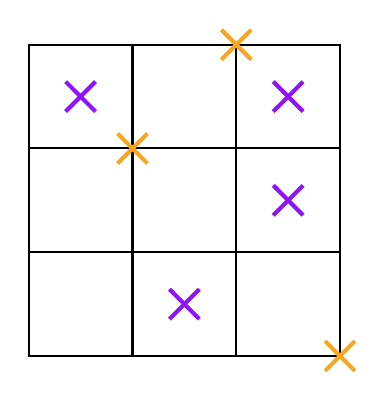
\begin{tikzpicture}[x=0.75pt,y=0.75pt,yscale=-1,xscale=1]
%uncomment if require: \path (0,300); %set diagram left start at 0, and has height of 300

%Shape: Square [id:dp4570817602982631] 
\draw   (100,29) -- (150,29) -- (150,79) -- (100,79) -- cycle ;
%Shape: Square [id:dp2903299358971252] 
\draw   (150,29) -- (200,29) -- (200,79) -- (150,79) -- cycle ;
%Shape: Square [id:dp8410481858286352] 
\draw   (100,79) -- (150,79) -- (150,129) -- (100,129) -- cycle ;
%Shape: Square [id:dp1117017430126368] 
\draw   (150,79) -- (200,79) -- (200,129) -- (150,129) -- cycle ;
%Shape: Square [id:dp9054195019818092] 
\draw   (200,29) -- (250,29) -- (250,79) -- (200,79) -- cycle ;
%Shape: Square [id:dp9918567360750739] 
\draw   (200,79) -- (250,79) -- (250,129) -- (200,129) -- cycle ;
%Shape: Square [id:dp6694249449139529] 
\draw   (100,129) -- (150,129) -- (150,179) -- (100,179) -- cycle ;
%Shape: Square [id:dp6467857772283392] 
\draw   (150,129) -- (200,129) -- (200,179) -- (150,179) -- cycle ;
%Shape: Square [id:dp32240121043282777] 
\draw   (200,129) -- (250,129) -- (250,179) -- (200,179) -- cycle ;
%Straight Lines [id:da5972676544083908] 
\draw [color={rgb, 255:red, 245; green, 166; blue, 35 }  ,draw opacity=1 ][line width=1.5]    (150,79) ;
\draw [shift={(150,79)}, rotate = 45] [color={rgb, 255:red, 245; green, 166; blue, 35 }  ,draw opacity=1 ][line width=1.5]    (-10.17,0) -- (10.17,0)(0,10.17) -- (0,-10.17)   ;
%Straight Lines [id:da06771970628563428] 
\draw [color={rgb, 255:red, 245; green, 166; blue, 35 }  ,draw opacity=1 ][line width=1.5]    (250,179) ;
\draw [shift={(250,179)}, rotate = 45] [color={rgb, 255:red, 245; green, 166; blue, 35 }  ,draw opacity=1 ][line width=1.5]    (-10.17,0) -- (10.17,0)(0,10.17) -- (0,-10.17)   ;
%Straight Lines [id:da1804222983474455] 
\draw [color={rgb, 255:red, 245; green, 166; blue, 35 }  ,draw opacity=1 ][line width=1.5]    (200,29) ;
\draw [shift={(200,29)}, rotate = 45] [color={rgb, 255:red, 245; green, 166; blue, 35 }  ,draw opacity=1 ][line width=1.5]    (-10.17,0) -- (10.17,0)(0,10.17) -- (0,-10.17)   ;
%Straight Lines [id:da7901030413597554] 
\draw [color={rgb, 255:red, 144; green, 19; blue, 254 }  ,draw opacity=1 ][line width=1.5]    (175,154) ;
\draw [shift={(175,154)}, rotate = 45] [color={rgb, 255:red, 144; green, 19; blue, 254 }  ,draw opacity=1 ][line width=1.5]    (-10.17,0) -- (10.17,0)(0,10.17) -- (0,-10.17)   ;
%Straight Lines [id:da37933960521297805] 
\draw [color={rgb, 255:red, 144; green, 19; blue, 254 }  ,draw opacity=1 ][line width=1.5]    (225,104) ;
\draw [shift={(225,104)}, rotate = 45] [color={rgb, 255:red, 144; green, 19; blue, 254 }  ,draw opacity=1 ][line width=1.5]    (-10.17,0) -- (10.17,0)(0,10.17) -- (0,-10.17)   ;
%Straight Lines [id:da13742234427535593] 
\draw [color={rgb, 255:red, 144; green, 19; blue, 254 }  ,draw opacity=1 ][line width=1.5]    (125,54) ;
\draw [shift={(125,54)}, rotate = 45] [color={rgb, 255:red, 144; green, 19; blue, 254 }  ,draw opacity=1 ][line width=1.5]    (-10.17,0) -- (10.17,0)(0,10.17) -- (0,-10.17)   ;
%Straight Lines [id:da5163777331330268] 
\draw [color={rgb, 255:red, 144; green, 19; blue, 254 }  ,draw opacity=1 ][line width=1.5]    (225,54) ;
\draw [shift={(225,54)}, rotate = 45] [color={rgb, 255:red, 144; green, 19; blue, 254 }  ,draw opacity=1 ][line width=1.5]    (-10.17,0) -- (10.17,0)(0,10.17) -- (0,-10.17)   ;




\end{tikzpicture}

    }
    \caption{Toric-code模型的系统构型和元激发}
\end{figure}

考虑一个正方晶格,在每条边(\emph{不是}每个格点!)上放有一个自旋$1/2$自由度。
哈密顿量为
\begin{equation}
    {H} = - \sum_s {A}_s - \sum_p {B}_p,
    \label{eq:toric-code-hamiltonian}
\end{equation}
其中下标$s$表示格点,${A}_s$指的是格点$s$周围的四条边上的$x$方向上的自旋算符的乘积,即
\begin{equation}
    {A}_s = \prod_{\vb*{i} \text{ near } s} {\sigma}_{\vb*{i}}^x,
\end{equation}
而$p$表示格点中的一个最小正方形方块,${B}_p$指的是正方形$p$的四条边上的$z$方向上的自旋算符的乘积,即
\begin{equation}
    {B}_p = \prod_\text{$\vb*{i}$ of $p$} {\sigma}_{\vb*{i}}^z.
\end{equation}

\eqref{eq:toric-code-hamiltonian}中显然有不小的量子涨落,因为有大量彼此不对易的算符。然而,我们将展示,它其实是严格可解的。
因此,Toric-code模型是一个很好的玩具模型,能够向我们展示量子涨落强烈的自旋系统的行为。

首先可以验证$\{{A}_s\}$和$\{{B}_p\}$构成一组对易稳定子(即平方为1的一组彼此对易的厄米算符),这样就有
\begin{equation}
    \comm*{{A}_s}{{H}} = \comm*{{B}_p}{{H}} = 0.
\end{equation}
另一方面,平方为1的厄米算符的本征值是$\pm 1$,于是我们就可以用它们的本征值$A_s = \pm 1$和$B_p = \pm 1$标记体系的能量本征态。
实际上,在热力学极限下只需要$\{A_s\}$和$\{B_p\}$就可以唯一地标记体系的能量本征态。
这是因为设体系有$N$个格点,那么有$4N/2=2N$条边,于是体系的希尔伯特空间的维数为$2^{2N}$。%
$s$和$p$均有$N$个,于是所有可能的$\{A_s\}$和$\{B_p\}$的组合总数为$2^N \cdot 2^N=2^{2N}$。
这样如果不考虑边界引入的微妙之处,只需要$\{A_s\}$和$\{B_p\}$就可以唯一地标记体系的能量本征态。
很容易看出体系的基态为所有$A_s$和$B_p$均为$1$的状态,于是我们可以把$A_s$和$B_p$为$-1$的情况看成激发态。这样我们就得到了\eqref{eq:toric-code-hamiltonian}的全部能量本征态,从而完全求解出了它。

显然Toric-code模型确实是自旋液体,因为其基态不具有任何经典意义上的序:我们得到的是一大堆$\sigma^x$确定的态和一大堆$\sigma^z$确定的态的线性叠加。

\subsection{环面上的情况}

\subsubsection{e激发和m激发}

为了解析求解,我们施加一个周期性边界条件,这相当于把体系放在了一个二维环面上。
此时诸$\{A_s\}$和$\{B_p\}$实际上不是彼此独立的,因为此时显然有
\[
    \prod_s {A}_s = 1,
\]
因为所有的$\{A_s\}$乘起来,每一条边被乘了两边,所以一定会得到$1$。类似的有
\[
    \prod_p {B}_p = 1.
\]
这两个方程要求
\begin{equation}
    \prod_{s} A_s = \prod_{p} B_p = 1.
    \label{eq:toric-code-pair-condition}
\end{equation}
这就意味着$A_s$激发和$B_p$激发必须成对出现,否则乘积将会是$-1$。我们将$A_s$激发称为e粒子,而将$B_p$激发称为m粒子,因为在某种意义上可以将$A_s$激发类比为电荷而将$B_p$激发理解为磁通量子。
这两种粒子的性质和空间的拓扑结构显然关系很大,因此称它们为拓扑激发。

\begin{figure}
    \centering
    \subfigure[将一个$O_\text{e}$开弦算符作用在一个元激发也没有的态上而得到的结果;弦两端出现了两个e激发]{
        

\tikzset{every picture/.style={line width=0.75pt}} %set default line width to 0.75pt        

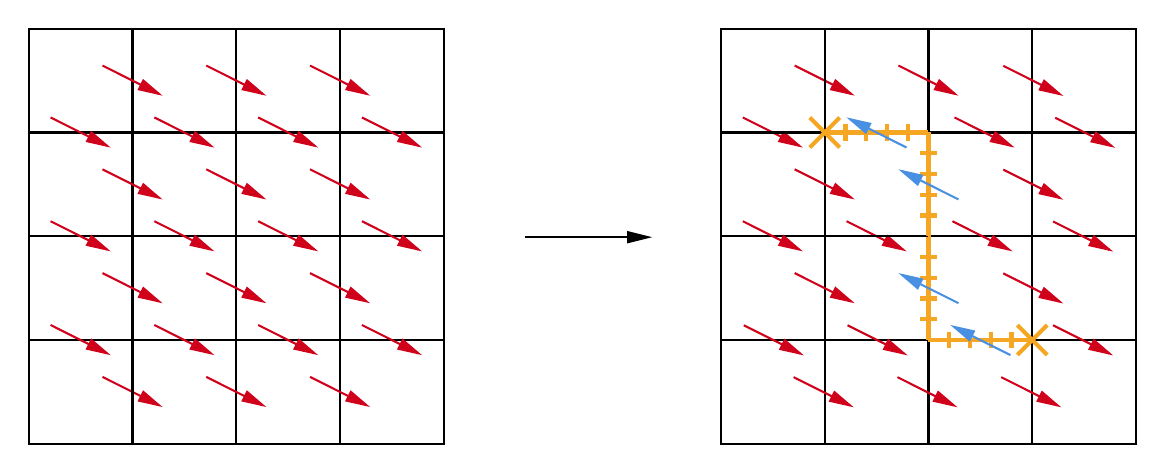
\begin{tikzpicture}[x=0.75pt,y=0.75pt,yscale=-1,xscale=1]
%uncomment if require: \path (0,300); %set diagram left start at 0, and has height of 300

%Shape: Square [id:dp3176853045406567] 
\draw   (413,192.06) -- (463,192.06) -- (463,242.06) -- (413,242.06) -- cycle ;
%Shape: Square [id:dp7022572838953951] 
\draw   (513,192.06) -- (563,192.06) -- (563,242.06) -- (513,242.06) -- cycle ;
%Shape: Square [id:dp030329102095208782] 
\draw   (513,142.06) -- (563,142.06) -- (563,192.06) -- (513,192.06) -- cycle ;
%Shape: Square [id:dp517134688980474] 
\draw   (463,192.06) -- (513,192.06) -- (513,242.06) -- (463,242.06) -- cycle ;
%Shape: Square [id:dp47682705008824966] 
\draw   (363,42.06) -- (413,42.06) -- (413,92.06) -- (363,92.06) -- cycle ;
%Shape: Square [id:dp40774233163885887] 
\draw   (413,42.06) -- (463,42.06) -- (463,92.06) -- (413,92.06) -- cycle ;
%Shape: Square [id:dp8421641317700328] 
\draw   (363,92.06) -- (413,92.06) -- (413,142.06) -- (363,142.06) -- cycle ;
%Shape: Square [id:dp8149136823625276] 
\draw   (413,92.06) -- (463,92.06) -- (463,142.06) -- (413,142.06) -- cycle ;
%Shape: Square [id:dp9420804931616191] 
\draw   (463,42.06) -- (513,42.06) -- (513,92.06) -- (463,92.06) -- cycle ;
%Shape: Square [id:dp575792276688039] 
\draw   (463,92.06) -- (513,92.06) -- (513,142.06) -- (463,142.06) -- cycle ;
%Shape: Square [id:dp604089614437928] 
\draw   (363,142.06) -- (413,142.06) -- (413,192.06) -- (363,192.06) -- cycle ;
%Shape: Square [id:dp9110252712752467] 
\draw   (413,142.06) -- (463,142.06) -- (463,192.06) -- (413,192.06) -- cycle ;
%Shape: Square [id:dp757512175683634] 
\draw   (463,142.06) -- (513,142.06) -- (513,192.06) -- (463,192.06) -- cycle ;
%Straight Lines [id:da24590588647520528] 
\draw [color={rgb, 255:red, 245; green, 166; blue, 35 }  ,draw opacity=1 ][line width=1.5]    (513,192.06) ;
\draw [shift={(513,192.06)}, rotate = 45] [color={rgb, 255:red, 245; green, 166; blue, 35 }  ,draw opacity=1 ][line width=1.5]    (-10.17,0) -- (10.17,0)(0,10.17) -- (0,-10.17)   ;
%Straight Lines [id:da734113367713265] 
\draw [color={rgb, 255:red, 245; green, 166; blue, 35 }  ,draw opacity=1 ][line width=1.5]    (463,192.06) -- (513,192.06) (473,188.06) -- (473,196.06)(483,188.06) -- (483,196.06)(493,188.06) -- (493,196.06)(503,188.06) -- (503,196.06) ;
%Straight Lines [id:da8677740521877175] 
\draw [color={rgb, 255:red, 245; green, 166; blue, 35 }  ,draw opacity=1 ][line width=1.5]    (463,192.06) -- (463,142.06) (459,182.06) -- (467,182.06)(459,172.06) -- (467,172.06)(459,162.06) -- (467,162.06)(459,152.06) -- (467,152.06) ;
%Straight Lines [id:da9217711157137525] 
\draw [color={rgb, 255:red, 208; green, 2; blue, 27 }  ,draw opacity=1 ]   (398.54,59.81) -- (425.67,73.42) ;
\draw [shift={(427.46,74.31)}, rotate = 206.63] [fill={rgb, 255:red, 208; green, 2; blue, 27 }  ,fill opacity=1 ][line width=0.08]  [draw opacity=0] (12,-3) -- (0,0) -- (12,3) -- cycle    ;
%Straight Lines [id:da8231785182807179] 
\draw    (413,42.06) -- (413,92.06) ;
%Straight Lines [id:da41308525995744727] 
\draw    (413,92.06) -- (413,142.06) ;
%Straight Lines [id:da3012120677599419] 
\draw [color={rgb, 255:red, 208; green, 2; blue, 27 }  ,draw opacity=1 ]   (373.54,84.81) -- (400.67,98.42) ;
\draw [shift={(402.46,99.31)}, rotate = 206.63] [fill={rgb, 255:red, 208; green, 2; blue, 27 }  ,fill opacity=1 ][line width=0.08]  [draw opacity=0] (12,-3) -- (0,0) -- (12,3) -- cycle    ;
%Straight Lines [id:da05997957846750057] 
\draw    (363,92.06) -- (413,92.06) ;
%Straight Lines [id:da3962017480147524] 
\draw [color={rgb, 255:red, 208; green, 2; blue, 27 }  ,draw opacity=1 ]   (398.54,109.81) -- (425.67,123.42) ;
\draw [shift={(427.46,124.31)}, rotate = 206.63] [fill={rgb, 255:red, 208; green, 2; blue, 27 }  ,fill opacity=1 ][line width=0.08]  [draw opacity=0] (12,-3) -- (0,0) -- (12,3) -- cycle    ;
%Straight Lines [id:da8887410805092772] 
\draw [color={rgb, 255:red, 74; green, 144; blue, 226 }  ,draw opacity=1 ]   (477.46,174.31) -- (450.33,160.71) ;
\draw [shift={(448.54,159.81)}, rotate = 386.63] [fill={rgb, 255:red, 74; green, 144; blue, 226 }  ,fill opacity=1 ][line width=0.08]  [draw opacity=0] (12,-3) -- (0,0) -- (12,3) -- cycle    ;
%Straight Lines [id:da3161585135502756] 
\draw [color={rgb, 255:red, 74; green, 144; blue, 226 }  ,draw opacity=1 ]   (502.46,199.31) -- (475.33,185.71) ;
\draw [shift={(473.54,184.81)}, rotate = 386.63] [fill={rgb, 255:red, 74; green, 144; blue, 226 }  ,fill opacity=1 ][line width=0.08]  [draw opacity=0] (12,-3) -- (0,0) -- (12,3) -- cycle    ;
%Straight Lines [id:da02918311398315465] 
\draw    (463,42.06) -- (463,92.06) ;
%Straight Lines [id:da2940193548924497] 
\draw [color={rgb, 255:red, 208; green, 2; blue, 27 }  ,draw opacity=1 ]   (448.54,59.81) -- (475.67,73.42) ;
\draw [shift={(477.46,74.31)}, rotate = 206.63] [fill={rgb, 255:red, 208; green, 2; blue, 27 }  ,fill opacity=1 ][line width=0.08]  [draw opacity=0] (12,-3) -- (0,0) -- (12,3) -- cycle    ;
%Straight Lines [id:da2999016051074743] 
\draw [color={rgb, 255:red, 208; green, 2; blue, 27 }  ,draw opacity=1 ]   (423.54,134.81) -- (450.67,148.42) ;
\draw [shift={(452.46,149.31)}, rotate = 206.63] [fill={rgb, 255:red, 208; green, 2; blue, 27 }  ,fill opacity=1 ][line width=0.08]  [draw opacity=0] (12,-3) -- (0,0) -- (12,3) -- cycle    ;
%Straight Lines [id:da13812102603223497] 
\draw    (413,142.06) -- (463,142.06) ;
%Straight Lines [id:da473115693085842] 
\draw [color={rgb, 255:red, 245; green, 166; blue, 35 }  ,draw opacity=1 ][line width=1.5]    (413,92.06) -- (463,92.06) (423,88.06) -- (423,96.06)(433,88.06) -- (433,96.06)(443,88.06) -- (443,96.06)(453,88.06) -- (453,96.06) ;
%Straight Lines [id:da21779160831084354] 
\draw [color={rgb, 255:red, 245; green, 166; blue, 35 }  ,draw opacity=1 ][line width=1.5]    (463,142.06) -- (463,92.06) (459,132.06) -- (467,132.06)(459,122.06) -- (467,122.06)(459,112.06) -- (467,112.06)(459,102.06) -- (467,102.06) ;
%Straight Lines [id:da08642153104428818] 
\draw    (363,142.06) -- (413,142.06) ;
%Straight Lines [id:da6951119379014274] 
\draw [color={rgb, 255:red, 208; green, 2; blue, 27 }  ,draw opacity=1 ]   (373.54,134.81) -- (400.67,148.42) ;
\draw [shift={(402.46,149.31)}, rotate = 206.63] [fill={rgb, 255:red, 208; green, 2; blue, 27 }  ,fill opacity=1 ][line width=0.08]  [draw opacity=0] (12,-3) -- (0,0) -- (12,3) -- cycle    ;
%Straight Lines [id:da08264979104155512] 
\draw    (413,142.06) -- (413,192.06) ;
%Straight Lines [id:da8129978724657629] 
\draw [color={rgb, 255:red, 208; green, 2; blue, 27 }  ,draw opacity=1 ]   (398.54,159.81) -- (425.67,173.42) ;
\draw [shift={(427.46,174.31)}, rotate = 206.63] [fill={rgb, 255:red, 208; green, 2; blue, 27 }  ,fill opacity=1 ][line width=0.08]  [draw opacity=0] (12,-3) -- (0,0) -- (12,3) -- cycle    ;
%Straight Lines [id:da16655027105891573] 
\draw [color={rgb, 255:red, 208; green, 2; blue, 27 }  ,draw opacity=1 ]   (474.54,134.81) -- (501.67,148.42) ;
\draw [shift={(503.46,149.31)}, rotate = 206.63] [fill={rgb, 255:red, 208; green, 2; blue, 27 }  ,fill opacity=1 ][line width=0.08]  [draw opacity=0] (12,-3) -- (0,0) -- (12,3) -- cycle    ;
%Straight Lines [id:da961269861360253] 
\draw [color={rgb, 255:red, 208; green, 2; blue, 27 }  ,draw opacity=1 ]   (475.54,84.81) -- (502.67,98.42) ;
\draw [shift={(504.46,99.31)}, rotate = 206.63] [fill={rgb, 255:red, 208; green, 2; blue, 27 }  ,fill opacity=1 ][line width=0.08]  [draw opacity=0] (12,-3) -- (0,0) -- (12,3) -- cycle    ;
%Straight Lines [id:da8577823672113685] 
\draw [color={rgb, 255:red, 74; green, 144; blue, 226 }  ,draw opacity=1 ]   (452.46,99.31) -- (425.33,85.71) ;
\draw [shift={(423.54,84.81)}, rotate = 386.63] [fill={rgb, 255:red, 74; green, 144; blue, 226 }  ,fill opacity=1 ][line width=0.08]  [draw opacity=0] (12,-3) -- (0,0) -- (12,3) -- cycle    ;
%Straight Lines [id:da682500900340755] 
\draw [color={rgb, 255:red, 74; green, 144; blue, 226 }  ,draw opacity=1 ]   (477.46,124.31) -- (450.33,110.71) ;
\draw [shift={(448.54,109.81)}, rotate = 386.63] [fill={rgb, 255:red, 74; green, 144; blue, 226 }  ,fill opacity=1 ][line width=0.08]  [draw opacity=0] (12,-3) -- (0,0) -- (12,3) -- cycle    ;
%Straight Lines [id:da09306781133035313] 
\draw [color={rgb, 255:red, 245; green, 166; blue, 35 }  ,draw opacity=1 ][line width=1.5]    (413,92.06) ;
\draw [shift={(413,92.06)}, rotate = 45] [color={rgb, 255:red, 245; green, 166; blue, 35 }  ,draw opacity=1 ][line width=1.5]    (-10.17,0) -- (10.17,0)(0,10.17) -- (0,-10.17)   ;

%Shape: Square [id:dp8465447023173558] 
\draw   (363,192.06) -- (413,192.06) -- (413,242.06) -- (363,242.06) -- cycle ;
%Shape: Square [id:dp9438298309585613] 
\draw   (513,42.06) -- (563,42.06) -- (563,92.06) -- (513,92.06) -- cycle ;
%Shape: Square [id:dp6994512173158287] 
\draw   (513,92.06) -- (563,92.06) -- (563,142.06) -- (513,142.06) -- cycle ;
%Straight Lines [id:da8418892124168778] 
\draw [color={rgb, 255:red, 208; green, 2; blue, 27 }  ,draw opacity=1 ]   (498.04,209.94) -- (525.17,223.54) ;
\draw [shift={(526.96,224.44)}, rotate = 206.63] [fill={rgb, 255:red, 208; green, 2; blue, 27 }  ,fill opacity=1 ][line width=0.08]  [draw opacity=0] (12,-3) -- (0,0) -- (12,3) -- cycle    ;
%Straight Lines [id:da9061042682723188] 
\draw [color={rgb, 255:red, 208; green, 2; blue, 27 }  ,draw opacity=1 ]   (448.04,209.94) -- (475.17,223.54) ;
\draw [shift={(476.96,224.44)}, rotate = 206.63] [fill={rgb, 255:red, 208; green, 2; blue, 27 }  ,fill opacity=1 ][line width=0.08]  [draw opacity=0] (12,-3) -- (0,0) -- (12,3) -- cycle    ;
%Straight Lines [id:da7687163300487452] 
\draw [color={rgb, 255:red, 208; green, 2; blue, 27 }  ,draw opacity=1 ]   (398.04,209.94) -- (425.17,223.54) ;
\draw [shift={(426.96,224.44)}, rotate = 206.63] [fill={rgb, 255:red, 208; green, 2; blue, 27 }  ,fill opacity=1 ][line width=0.08]  [draw opacity=0] (12,-3) -- (0,0) -- (12,3) -- cycle    ;
%Straight Lines [id:da22859514957556426] 
\draw    (512.5,92.19) -- (562.5,92.19) ;
%Straight Lines [id:da8368486354382343] 
\draw [color={rgb, 255:red, 208; green, 2; blue, 27 }  ,draw opacity=1 ]   (523.04,134.94) -- (550.17,148.54) ;
\draw [shift={(551.96,149.44)}, rotate = 206.63] [fill={rgb, 255:red, 208; green, 2; blue, 27 }  ,fill opacity=1 ][line width=0.08]  [draw opacity=0] (12,-3) -- (0,0) -- (12,3) -- cycle    ;
%Straight Lines [id:da284559803269298] 
\draw [color={rgb, 255:red, 208; green, 2; blue, 27 }  ,draw opacity=1 ]   (523.04,184.94) -- (550.17,198.54) ;
\draw [shift={(551.96,199.44)}, rotate = 206.63] [fill={rgb, 255:red, 208; green, 2; blue, 27 }  ,fill opacity=1 ][line width=0.08]  [draw opacity=0] (12,-3) -- (0,0) -- (12,3) -- cycle    ;
%Straight Lines [id:da7109167776610843] 
\draw [color={rgb, 255:red, 208; green, 2; blue, 27 }  ,draw opacity=1 ]   (374.04,184.94) -- (401.17,198.54) ;
\draw [shift={(402.96,199.44)}, rotate = 206.63] [fill={rgb, 255:red, 208; green, 2; blue, 27 }  ,fill opacity=1 ][line width=0.08]  [draw opacity=0] (12,-3) -- (0,0) -- (12,3) -- cycle    ;
%Straight Lines [id:da7975065936613515] 
\draw [color={rgb, 255:red, 208; green, 2; blue, 27 }  ,draw opacity=1 ]   (524.04,84.94) -- (551.17,98.54) ;
\draw [shift={(552.96,99.44)}, rotate = 206.63] [fill={rgb, 255:red, 208; green, 2; blue, 27 }  ,fill opacity=1 ][line width=0.08]  [draw opacity=0] (12,-3) -- (0,0) -- (12,3) -- cycle    ;
%Straight Lines [id:da1414304216799871] 
\draw [color={rgb, 255:red, 208; green, 2; blue, 27 }  ,draw opacity=1 ]   (424.04,184.94) -- (451.17,198.54) ;
\draw [shift={(452.96,199.44)}, rotate = 206.63] [fill={rgb, 255:red, 208; green, 2; blue, 27 }  ,fill opacity=1 ][line width=0.08]  [draw opacity=0] (12,-3) -- (0,0) -- (12,3) -- cycle    ;
%Straight Lines [id:da0049146308443612785] 
\draw [color={rgb, 255:red, 208; green, 2; blue, 27 }  ,draw opacity=1 ]   (499.04,109.94) -- (526.17,123.54) ;
\draw [shift={(527.96,124.44)}, rotate = 206.63] [fill={rgb, 255:red, 208; green, 2; blue, 27 }  ,fill opacity=1 ][line width=0.08]  [draw opacity=0] (12,-3) -- (0,0) -- (12,3) -- cycle    ;
%Straight Lines [id:da45851520453208705] 
\draw [color={rgb, 255:red, 208; green, 2; blue, 27 }  ,draw opacity=1 ]   (499.04,159.94) -- (526.17,173.54) ;
\draw [shift={(527.96,174.44)}, rotate = 206.63] [fill={rgb, 255:red, 208; green, 2; blue, 27 }  ,fill opacity=1 ][line width=0.08]  [draw opacity=0] (12,-3) -- (0,0) -- (12,3) -- cycle    ;
%Straight Lines [id:da193368586544167] 
\draw [color={rgb, 255:red, 208; green, 2; blue, 27 }  ,draw opacity=1 ]   (499.04,59.94) -- (526.17,73.54) ;
\draw [shift={(527.96,74.44)}, rotate = 206.63] [fill={rgb, 255:red, 208; green, 2; blue, 27 }  ,fill opacity=1 ][line width=0.08]  [draw opacity=0] (12,-3) -- (0,0) -- (12,3) -- cycle    ;
%Shape: Square [id:dp2944681179982789] 
\draw   (29.5,42.06) -- (79.5,42.06) -- (79.5,92.06) -- (29.5,92.06) -- cycle ;
%Shape: Square [id:dp9907886405428181] 
\draw   (79.5,42.06) -- (129.5,42.06) -- (129.5,92.06) -- (79.5,92.06) -- cycle ;
%Shape: Square [id:dp6519502476448713] 
\draw   (29.5,92.06) -- (79.5,92.06) -- (79.5,142.06) -- (29.5,142.06) -- cycle ;
%Shape: Square [id:dp7925682746127443] 
\draw   (79.5,92.06) -- (129.5,92.06) -- (129.5,142.06) -- (79.5,142.06) -- cycle ;
%Shape: Square [id:dp5442048196323481] 
\draw   (129.5,42.06) -- (179.5,42.06) -- (179.5,92.06) -- (129.5,92.06) -- cycle ;
%Shape: Square [id:dp25248026898484044] 
\draw   (129.5,92.06) -- (179.5,92.06) -- (179.5,142.06) -- (129.5,142.06) -- cycle ;
%Shape: Square [id:dp7775590480268038] 
\draw   (29.5,142.06) -- (79.5,142.06) -- (79.5,192.06) -- (29.5,192.06) -- cycle ;
%Shape: Square [id:dp1338343200880323] 
\draw   (79.5,142.06) -- (129.5,142.06) -- (129.5,192.06) -- (79.5,192.06) -- cycle ;
%Shape: Square [id:dp7088532821434324] 
\draw   (129.5,142.06) -- (179.5,142.06) -- (179.5,192.06) -- (129.5,192.06) -- cycle ;
%Straight Lines [id:da2700497890258473] 
\draw    (79.5,42.06) -- (79.5,92.06) ;
%Straight Lines [id:da2937434592243895] 
\draw    (79.5,92.06) -- (79.5,142.06) ;
%Straight Lines [id:da32767216765463614] 
\draw    (29.5,92.06) -- (79.5,92.06) ;
%Straight Lines [id:da2701106509000726] 
\draw    (129.5,42.06) -- (129.5,92.06) ;
%Straight Lines [id:da28944079432298353] 
\draw    (79.5,142.06) -- (129.5,142.06) ;
%Straight Lines [id:da7898411476311509] 
\draw    (29.5,142.06) -- (79.5,142.06) ;
%Straight Lines [id:da03266817725577198] 
\draw    (79.5,142.06) -- (79.5,192.06) ;
%Straight Lines [id:da8791797326384476] 
\draw [color={rgb, 255:red, 208; green, 2; blue, 27 }  ,draw opacity=1 ]   (65.04,59.81) -- (92.17,73.42) ;
\draw [shift={(93.96,74.31)}, rotate = 206.63] [fill={rgb, 255:red, 208; green, 2; blue, 27 }  ,fill opacity=1 ][line width=0.08]  [draw opacity=0] (12,-3) -- (0,0) -- (12,3) -- cycle    ;
%Straight Lines [id:da14031419653980737] 
\draw    (129.5,92.06) -- (129.5,142.06) ;
%Straight Lines [id:da5977365206916692] 
\draw    (129.5,142.06) -- (129.5,192.06) ;
%Straight Lines [id:da9839694802864396] 
\draw    (129.5,92.06) -- (179.5,92.06) ;
%Straight Lines [id:da018334436378720564] 
\draw    (129.5,142.06) -- (179.5,142.06) ;
%Straight Lines [id:da09894691687093027] 
\draw    (79.5,92.06) -- (129.5,92.06) ;
%Straight Lines [id:da9778402930655135] 
\draw [color={rgb, 255:red, 208; green, 2; blue, 27 }  ,draw opacity=1 ]   (115.04,59.81) -- (142.17,73.42) ;
\draw [shift={(143.96,74.31)}, rotate = 206.63] [fill={rgb, 255:red, 208; green, 2; blue, 27 }  ,fill opacity=1 ][line width=0.08]  [draw opacity=0] (12,-3) -- (0,0) -- (12,3) -- cycle    ;
%Straight Lines [id:da13706788423900362] 
\draw [color={rgb, 255:red, 208; green, 2; blue, 27 }  ,draw opacity=1 ]   (90.04,84.81) -- (117.17,98.42) ;
\draw [shift={(118.96,99.31)}, rotate = 206.63] [fill={rgb, 255:red, 208; green, 2; blue, 27 }  ,fill opacity=1 ][line width=0.08]  [draw opacity=0] (12,-3) -- (0,0) -- (12,3) -- cycle    ;
%Straight Lines [id:da07422420860788348] 
\draw [color={rgb, 255:red, 208; green, 2; blue, 27 }  ,draw opacity=1 ]   (40.04,84.81) -- (67.17,98.42) ;
\draw [shift={(68.96,99.31)}, rotate = 206.63] [fill={rgb, 255:red, 208; green, 2; blue, 27 }  ,fill opacity=1 ][line width=0.08]  [draw opacity=0] (12,-3) -- (0,0) -- (12,3) -- cycle    ;
%Straight Lines [id:da266151243916958] 
\draw [color={rgb, 255:red, 208; green, 2; blue, 27 }  ,draw opacity=1 ]   (140.04,84.81) -- (167.17,98.42) ;
\draw [shift={(168.96,99.31)}, rotate = 206.63] [fill={rgb, 255:red, 208; green, 2; blue, 27 }  ,fill opacity=1 ][line width=0.08]  [draw opacity=0] (12,-3) -- (0,0) -- (12,3) -- cycle    ;
%Straight Lines [id:da7305761483239985] 
\draw [color={rgb, 255:red, 208; green, 2; blue, 27 }  ,draw opacity=1 ]   (65.04,109.81) -- (92.17,123.42) ;
\draw [shift={(93.96,124.31)}, rotate = 206.63] [fill={rgb, 255:red, 208; green, 2; blue, 27 }  ,fill opacity=1 ][line width=0.08]  [draw opacity=0] (12,-3) -- (0,0) -- (12,3) -- cycle    ;
%Straight Lines [id:da26390191757327797] 
\draw [color={rgb, 255:red, 208; green, 2; blue, 27 }  ,draw opacity=1 ]   (115.04,109.81) -- (142.17,123.42) ;
\draw [shift={(143.96,124.31)}, rotate = 206.63] [fill={rgb, 255:red, 208; green, 2; blue, 27 }  ,fill opacity=1 ][line width=0.08]  [draw opacity=0] (12,-3) -- (0,0) -- (12,3) -- cycle    ;
%Straight Lines [id:da39405663144228087] 
\draw [color={rgb, 255:red, 208; green, 2; blue, 27 }  ,draw opacity=1 ]   (90.04,134.81) -- (117.17,148.42) ;
\draw [shift={(118.96,149.31)}, rotate = 206.63] [fill={rgb, 255:red, 208; green, 2; blue, 27 }  ,fill opacity=1 ][line width=0.08]  [draw opacity=0] (12,-3) -- (0,0) -- (12,3) -- cycle    ;
%Straight Lines [id:da4635634803052915] 
\draw [color={rgb, 255:red, 208; green, 2; blue, 27 }  ,draw opacity=1 ]   (140.04,134.81) -- (167.17,148.42) ;
\draw [shift={(168.96,149.31)}, rotate = 206.63] [fill={rgb, 255:red, 208; green, 2; blue, 27 }  ,fill opacity=1 ][line width=0.08]  [draw opacity=0] (12,-3) -- (0,0) -- (12,3) -- cycle    ;
%Straight Lines [id:da5943890262371219] 
\draw [color={rgb, 255:red, 208; green, 2; blue, 27 }  ,draw opacity=1 ]   (40.04,134.81) -- (67.17,148.42) ;
\draw [shift={(68.96,149.31)}, rotate = 206.63] [fill={rgb, 255:red, 208; green, 2; blue, 27 }  ,fill opacity=1 ][line width=0.08]  [draw opacity=0] (12,-3) -- (0,0) -- (12,3) -- cycle    ;
%Straight Lines [id:da6028394051065804] 
\draw [color={rgb, 255:red, 208; green, 2; blue, 27 }  ,draw opacity=1 ]   (65.04,159.81) -- (92.17,173.42) ;
\draw [shift={(93.96,174.31)}, rotate = 206.63] [fill={rgb, 255:red, 208; green, 2; blue, 27 }  ,fill opacity=1 ][line width=0.08]  [draw opacity=0] (12,-3) -- (0,0) -- (12,3) -- cycle    ;
%Straight Lines [id:da507884443037212] 
\draw [color={rgb, 255:red, 208; green, 2; blue, 27 }  ,draw opacity=1 ]   (115.04,159.81) -- (142.17,173.42) ;
\draw [shift={(143.96,174.31)}, rotate = 206.63] [fill={rgb, 255:red, 208; green, 2; blue, 27 }  ,fill opacity=1 ][line width=0.08]  [draw opacity=0] (12,-3) -- (0,0) -- (12,3) -- cycle    ;
%Straight Lines [id:da23526586798373939] 
\draw    (179.5,42.06) -- (179.5,92.06) ;
%Shape: Square [id:dp6143206523167073] 
\draw   (179.5,92.06) -- (229.5,92.06) -- (229.5,142.06) -- (179.5,142.06) -- cycle ;
%Shape: Square [id:dp0985246562755] 
\draw   (179.5,142.06) -- (229.5,142.06) -- (229.5,192.06) -- (179.5,192.06) -- cycle ;
%Shape: Square [id:dp6484371579778048] 
\draw   (179.5,42.06) -- (229.5,42.06) -- (229.5,92.06) -- (179.5,92.06) -- cycle ;
%Shape: Square [id:dp8586906674689465] 
\draw   (29.5,192.06) -- (79.5,192.06) -- (79.5,242.06) -- (29.5,242.06) -- cycle ;
%Shape: Square [id:dp04872184355539333] 
\draw   (79.5,192.06) -- (129.5,192.06) -- (129.5,242.06) -- (79.5,242.06) -- cycle ;
%Shape: Square [id:dp3103882786233412] 
\draw   (129.5,192.06) -- (179.5,192.06) -- (179.5,242.06) -- (129.5,242.06) -- cycle ;
%Shape: Square [id:dp0013830975332691509] 
\draw   (179.5,192.06) -- (229.5,192.06) -- (229.5,242.06) -- (179.5,242.06) -- cycle ;
%Straight Lines [id:da014561450380517149] 
\draw [color={rgb, 255:red, 208; green, 2; blue, 27 }  ,draw opacity=1 ]   (165.04,59.81) -- (192.17,73.42) ;
\draw [shift={(193.96,74.31)}, rotate = 206.63] [fill={rgb, 255:red, 208; green, 2; blue, 27 }  ,fill opacity=1 ][line width=0.08]  [draw opacity=0] (12,-3) -- (0,0) -- (12,3) -- cycle    ;
%Straight Lines [id:da8815895180727022] 
\draw    (179.5,92.06) -- (179.5,142.06) ;
%Straight Lines [id:da8964099918644335] 
\draw    (179.5,142.06) -- (179.5,192.06) ;
%Straight Lines [id:da7565582718111021] 
\draw    (179.5,192.06) -- (179.5,242.06) ;
%Straight Lines [id:da803623427369047] 
\draw    (129.5,192.06) -- (129.5,242.06) ;
%Straight Lines [id:da11895860097793509] 
\draw    (79.5,192.06) -- (79.5,242.06) ;
%Straight Lines [id:da05456314898380055] 
\draw [color={rgb, 255:red, 208; green, 2; blue, 27 }  ,draw opacity=1 ]   (165.04,109.81) -- (192.17,123.42) ;
\draw [shift={(193.96,124.31)}, rotate = 206.63] [fill={rgb, 255:red, 208; green, 2; blue, 27 }  ,fill opacity=1 ][line width=0.08]  [draw opacity=0] (12,-3) -- (0,0) -- (12,3) -- cycle    ;
%Straight Lines [id:da08984875889216193] 
\draw [color={rgb, 255:red, 208; green, 2; blue, 27 }  ,draw opacity=1 ]   (165.04,159.81) -- (192.17,173.42) ;
\draw [shift={(193.96,174.31)}, rotate = 206.63] [fill={rgb, 255:red, 208; green, 2; blue, 27 }  ,fill opacity=1 ][line width=0.08]  [draw opacity=0] (12,-3) -- (0,0) -- (12,3) -- cycle    ;
%Straight Lines [id:da6784600873216933] 
\draw [color={rgb, 255:red, 208; green, 2; blue, 27 }  ,draw opacity=1 ]   (165.04,209.81) -- (192.17,223.42) ;
\draw [shift={(193.96,224.31)}, rotate = 206.63] [fill={rgb, 255:red, 208; green, 2; blue, 27 }  ,fill opacity=1 ][line width=0.08]  [draw opacity=0] (12,-3) -- (0,0) -- (12,3) -- cycle    ;
%Straight Lines [id:da8487115371584568] 
\draw [color={rgb, 255:red, 208; green, 2; blue, 27 }  ,draw opacity=1 ]   (115.04,209.81) -- (142.17,223.42) ;
\draw [shift={(143.96,224.31)}, rotate = 206.63] [fill={rgb, 255:red, 208; green, 2; blue, 27 }  ,fill opacity=1 ][line width=0.08]  [draw opacity=0] (12,-3) -- (0,0) -- (12,3) -- cycle    ;
%Straight Lines [id:da9939290930501483] 
\draw [color={rgb, 255:red, 208; green, 2; blue, 27 }  ,draw opacity=1 ]   (65.04,209.81) -- (92.17,223.42) ;
\draw [shift={(93.96,224.31)}, rotate = 206.63] [fill={rgb, 255:red, 208; green, 2; blue, 27 }  ,fill opacity=1 ][line width=0.08]  [draw opacity=0] (12,-3) -- (0,0) -- (12,3) -- cycle    ;
%Straight Lines [id:da8839808429975873] 
\draw    (79.5,192.06) -- (79.5,242.06) ;
%Straight Lines [id:da1812289236897746] 
\draw    (29.5,192.06) -- (79.5,192.06) ;
%Straight Lines [id:da040898188258963186] 
\draw    (179.5,92.06) -- (229.5,92.06) ;
%Straight Lines [id:da14970457661241787] 
\draw    (179.5,142.06) -- (229.5,142.06) ;
%Straight Lines [id:da7190142368090202] 
\draw    (179.5,192.06) -- (229.5,192.06) ;
%Straight Lines [id:da10931629209917415] 
\draw [color={rgb, 255:red, 208; green, 2; blue, 27 }  ,draw opacity=1 ]   (40.04,184.81) -- (67.17,198.42) ;
\draw [shift={(68.96,199.31)}, rotate = 206.63] [fill={rgb, 255:red, 208; green, 2; blue, 27 }  ,fill opacity=1 ][line width=0.08]  [draw opacity=0] (12,-3) -- (0,0) -- (12,3) -- cycle    ;
%Straight Lines [id:da5189764682263813] 
\draw [color={rgb, 255:red, 208; green, 2; blue, 27 }  ,draw opacity=1 ]   (190.04,84.81) -- (217.17,98.42) ;
\draw [shift={(218.96,99.31)}, rotate = 206.63] [fill={rgb, 255:red, 208; green, 2; blue, 27 }  ,fill opacity=1 ][line width=0.08]  [draw opacity=0] (12,-3) -- (0,0) -- (12,3) -- cycle    ;
%Straight Lines [id:da011081053849876676] 
\draw [color={rgb, 255:red, 208; green, 2; blue, 27 }  ,draw opacity=1 ]   (190.04,134.81) -- (217.17,148.42) ;
\draw [shift={(218.96,149.31)}, rotate = 206.63] [fill={rgb, 255:red, 208; green, 2; blue, 27 }  ,fill opacity=1 ][line width=0.08]  [draw opacity=0] (12,-3) -- (0,0) -- (12,3) -- cycle    ;
%Straight Lines [id:da7442504430853205] 
\draw [color={rgb, 255:red, 208; green, 2; blue, 27 }  ,draw opacity=1 ]   (190.04,184.81) -- (217.17,198.42) ;
\draw [shift={(218.96,199.31)}, rotate = 206.63] [fill={rgb, 255:red, 208; green, 2; blue, 27 }  ,fill opacity=1 ][line width=0.08]  [draw opacity=0] (12,-3) -- (0,0) -- (12,3) -- cycle    ;
%Straight Lines [id:da3970407070395152] 
\draw    (79.5,192.06) -- (129.5,192.06) ;
%Straight Lines [id:da6055180132972338] 
\draw    (129.5,192.06) -- (179.5,192.06) ;
%Straight Lines [id:da6938740383021329] 
\draw [color={rgb, 255:red, 208; green, 2; blue, 27 }  ,draw opacity=1 ]   (140.04,184.81) -- (167.17,198.42) ;
\draw [shift={(168.96,199.31)}, rotate = 206.63] [fill={rgb, 255:red, 208; green, 2; blue, 27 }  ,fill opacity=1 ][line width=0.08]  [draw opacity=0] (12,-3) -- (0,0) -- (12,3) -- cycle    ;
%Straight Lines [id:da3372631654864733] 
\draw [color={rgb, 255:red, 208; green, 2; blue, 27 }  ,draw opacity=1 ]   (90.04,184.81) -- (117.17,198.42) ;
\draw [shift={(118.96,199.31)}, rotate = 206.63] [fill={rgb, 255:red, 208; green, 2; blue, 27 }  ,fill opacity=1 ][line width=0.08]  [draw opacity=0] (12,-3) -- (0,0) -- (12,3) -- cycle    ;

%Straight Lines [id:da2663235352080846] 
\draw    (268.83,142.5) -- (327.83,142.5) ;
\draw [shift={(329.83,142.5)}, rotate = 180] [fill={rgb, 255:red, 0; green, 0; blue, 0 }  ][line width=0.08]  [draw opacity=0] (12,-3) -- (0,0) -- (12,3) -- cycle    ;




\end{tikzpicture}

    }
    \subfigure[将一个$O_\text{e}$开弦算符作用在已有元激发的态上得到的结果;弦开头处的e激发被运送到了弦末尾,弦上其它各点上如果原本没有e激发,那么还是没有,如果原本有,那么现在还是有]{
        

\tikzset{every picture/.style={line width=0.75pt}} %set default line width to 0.75pt        

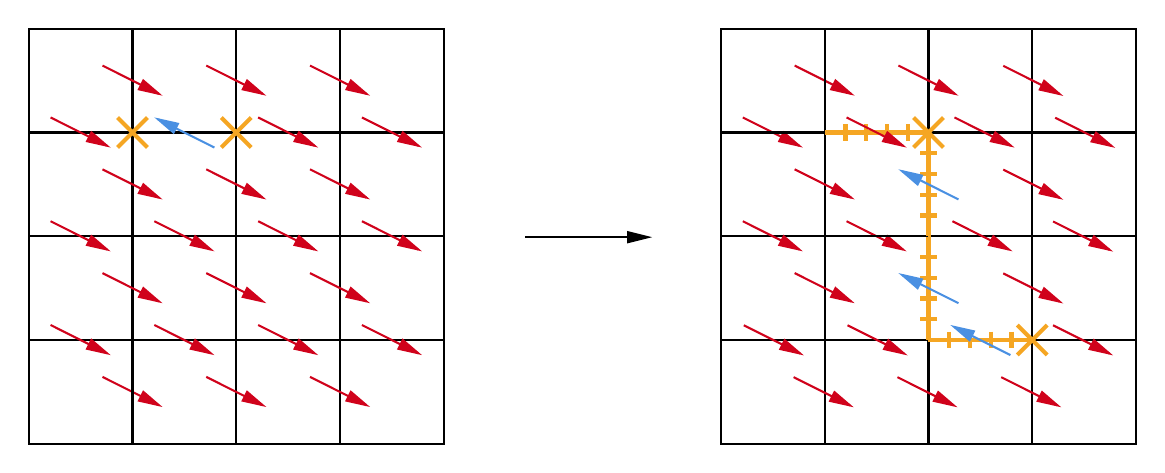
\begin{tikzpicture}[x=0.75pt,y=0.75pt,yscale=-1,xscale=1]
%uncomment if require: \path (0,300); %set diagram left start at 0, and has height of 300

%Shape: Square [id:dp36196949269788203] 
\draw   (433,212.06) -- (483,212.06) -- (483,262.06) -- (433,262.06) -- cycle ;
%Shape: Square [id:dp4539886973873315] 
\draw   (533,212.06) -- (583,212.06) -- (583,262.06) -- (533,262.06) -- cycle ;
%Shape: Square [id:dp6375978130473219] 
\draw   (533,162.06) -- (583,162.06) -- (583,212.06) -- (533,212.06) -- cycle ;
%Shape: Square [id:dp5485656687226403] 
\draw   (483,212.06) -- (533,212.06) -- (533,262.06) -- (483,262.06) -- cycle ;
%Shape: Square [id:dp7861946257195895] 
\draw   (383,62.06) -- (433,62.06) -- (433,112.06) -- (383,112.06) -- cycle ;
%Shape: Square [id:dp4265689791603251] 
\draw   (433,62.06) -- (483,62.06) -- (483,112.06) -- (433,112.06) -- cycle ;
%Shape: Square [id:dp85770876091055] 
\draw   (383,112.06) -- (433,112.06) -- (433,162.06) -- (383,162.06) -- cycle ;
%Shape: Square [id:dp9994589809447718] 
\draw   (433,112.06) -- (483,112.06) -- (483,162.06) -- (433,162.06) -- cycle ;
%Shape: Square [id:dp3934144084207285] 
\draw   (483,62.06) -- (533,62.06) -- (533,112.06) -- (483,112.06) -- cycle ;
%Shape: Square [id:dp44660161866059256] 
\draw   (483,112.06) -- (533,112.06) -- (533,162.06) -- (483,162.06) -- cycle ;
%Shape: Square [id:dp8655676597107462] 
\draw   (383,162.06) -- (433,162.06) -- (433,212.06) -- (383,212.06) -- cycle ;
%Shape: Square [id:dp31081007435708097] 
\draw   (433,162.06) -- (483,162.06) -- (483,212.06) -- (433,212.06) -- cycle ;
%Shape: Square [id:dp8086659149268767] 
\draw   (483,162.06) -- (533,162.06) -- (533,212.06) -- (483,212.06) -- cycle ;
%Straight Lines [id:da053200549000906205] 
\draw [color={rgb, 255:red, 245; green, 166; blue, 35 }  ,draw opacity=1 ][line width=1.5]    (533,212.06) ;
\draw [shift={(533,212.06)}, rotate = 45] [color={rgb, 255:red, 245; green, 166; blue, 35 }  ,draw opacity=1 ][line width=1.5]    (-10.17,0) -- (10.17,0)(0,10.17) -- (0,-10.17)   ;
%Straight Lines [id:da3649892359785114] 
\draw [color={rgb, 255:red, 245; green, 166; blue, 35 }  ,draw opacity=1 ][line width=1.5]    (483,212.06) -- (533,212.06) (493,208.06) -- (493,216.06)(503,208.06) -- (503,216.06)(513,208.06) -- (513,216.06)(523,208.06) -- (523,216.06) ;
%Straight Lines [id:da13469057648466287] 
\draw [color={rgb, 255:red, 245; green, 166; blue, 35 }  ,draw opacity=1 ][line width=1.5]    (483,212.06) -- (483,162.06) (479,202.06) -- (487,202.06)(479,192.06) -- (487,192.06)(479,182.06) -- (487,182.06)(479,172.06) -- (487,172.06) ;
%Straight Lines [id:da6345763045380002] 
\draw [color={rgb, 255:red, 208; green, 2; blue, 27 }  ,draw opacity=1 ]   (418.54,79.81) -- (445.67,93.42) ;
\draw [shift={(447.46,94.31)}, rotate = 206.63] [fill={rgb, 255:red, 208; green, 2; blue, 27 }  ,fill opacity=1 ][line width=0.08]  [draw opacity=0] (12,-3) -- (0,0) -- (12,3) -- cycle    ;
%Straight Lines [id:da5007686616056861] 
\draw    (433,62.06) -- (433,112.06) ;
%Straight Lines [id:da49682550012597915] 
\draw    (433,112.06) -- (433,162.06) ;
%Straight Lines [id:da9160145620735776] 
\draw [color={rgb, 255:red, 208; green, 2; blue, 27 }  ,draw opacity=1 ]   (393.54,104.81) -- (420.67,118.42) ;
\draw [shift={(422.46,119.31)}, rotate = 206.63] [fill={rgb, 255:red, 208; green, 2; blue, 27 }  ,fill opacity=1 ][line width=0.08]  [draw opacity=0] (12,-3) -- (0,0) -- (12,3) -- cycle    ;
%Straight Lines [id:da6394802587540938] 
\draw    (383,112.06) -- (433,112.06) ;
%Straight Lines [id:da32113469950640705] 
\draw [color={rgb, 255:red, 208; green, 2; blue, 27 }  ,draw opacity=1 ]   (418.54,129.81) -- (445.67,143.42) ;
\draw [shift={(447.46,144.31)}, rotate = 206.63] [fill={rgb, 255:red, 208; green, 2; blue, 27 }  ,fill opacity=1 ][line width=0.08]  [draw opacity=0] (12,-3) -- (0,0) -- (12,3) -- cycle    ;
%Straight Lines [id:da24099776716939703] 
\draw [color={rgb, 255:red, 74; green, 144; blue, 226 }  ,draw opacity=1 ]   (497.46,194.31) -- (470.33,180.71) ;
\draw [shift={(468.54,179.81)}, rotate = 386.63] [fill={rgb, 255:red, 74; green, 144; blue, 226 }  ,fill opacity=1 ][line width=0.08]  [draw opacity=0] (12,-3) -- (0,0) -- (12,3) -- cycle    ;
%Straight Lines [id:da5688629141790045] 
\draw [color={rgb, 255:red, 74; green, 144; blue, 226 }  ,draw opacity=1 ]   (522.46,219.31) -- (495.33,205.71) ;
\draw [shift={(493.54,204.81)}, rotate = 386.63] [fill={rgb, 255:red, 74; green, 144; blue, 226 }  ,fill opacity=1 ][line width=0.08]  [draw opacity=0] (12,-3) -- (0,0) -- (12,3) -- cycle    ;
%Straight Lines [id:da06719454989257079] 
\draw    (483,62.06) -- (483,112.06) ;
%Straight Lines [id:da3658940630124152] 
\draw [color={rgb, 255:red, 208; green, 2; blue, 27 }  ,draw opacity=1 ]   (468.54,79.81) -- (495.67,93.42) ;
\draw [shift={(497.46,94.31)}, rotate = 206.63] [fill={rgb, 255:red, 208; green, 2; blue, 27 }  ,fill opacity=1 ][line width=0.08]  [draw opacity=0] (12,-3) -- (0,0) -- (12,3) -- cycle    ;
%Straight Lines [id:da9827136653687769] 
\draw [color={rgb, 255:red, 208; green, 2; blue, 27 }  ,draw opacity=1 ]   (443.54,154.81) -- (470.67,168.42) ;
\draw [shift={(472.46,169.31)}, rotate = 206.63] [fill={rgb, 255:red, 208; green, 2; blue, 27 }  ,fill opacity=1 ][line width=0.08]  [draw opacity=0] (12,-3) -- (0,0) -- (12,3) -- cycle    ;
%Straight Lines [id:da24542517630533744] 
\draw    (433,162.06) -- (483,162.06) ;
%Straight Lines [id:da675706435803094] 
\draw [color={rgb, 255:red, 245; green, 166; blue, 35 }  ,draw opacity=1 ][line width=1.5]    (433,112.06) -- (483,112.06) (443,108.06) -- (443,116.06)(453,108.06) -- (453,116.06)(463,108.06) -- (463,116.06)(473,108.06) -- (473,116.06) ;
%Straight Lines [id:da7807078761743926] 
\draw [color={rgb, 255:red, 245; green, 166; blue, 35 }  ,draw opacity=1 ][line width=1.5]    (483,162.06) -- (483,112.06) (479,152.06) -- (487,152.06)(479,142.06) -- (487,142.06)(479,132.06) -- (487,132.06)(479,122.06) -- (487,122.06) ;
%Straight Lines [id:da49273110414826204] 
\draw    (383,162.06) -- (433,162.06) ;
%Straight Lines [id:da4909188469525809] 
\draw [color={rgb, 255:red, 208; green, 2; blue, 27 }  ,draw opacity=1 ]   (393.54,154.81) -- (420.67,168.42) ;
\draw [shift={(422.46,169.31)}, rotate = 206.63] [fill={rgb, 255:red, 208; green, 2; blue, 27 }  ,fill opacity=1 ][line width=0.08]  [draw opacity=0] (12,-3) -- (0,0) -- (12,3) -- cycle    ;
%Straight Lines [id:da7732976407163501] 
\draw    (433,162.06) -- (433,212.06) ;
%Straight Lines [id:da8885840601877579] 
\draw [color={rgb, 255:red, 208; green, 2; blue, 27 }  ,draw opacity=1 ]   (418.54,179.81) -- (445.67,193.42) ;
\draw [shift={(447.46,194.31)}, rotate = 206.63] [fill={rgb, 255:red, 208; green, 2; blue, 27 }  ,fill opacity=1 ][line width=0.08]  [draw opacity=0] (12,-3) -- (0,0) -- (12,3) -- cycle    ;
%Straight Lines [id:da7563618305941129] 
\draw [color={rgb, 255:red, 208; green, 2; blue, 27 }  ,draw opacity=1 ]   (494.54,154.81) -- (521.67,168.42) ;
\draw [shift={(523.46,169.31)}, rotate = 206.63] [fill={rgb, 255:red, 208; green, 2; blue, 27 }  ,fill opacity=1 ][line width=0.08]  [draw opacity=0] (12,-3) -- (0,0) -- (12,3) -- cycle    ;
%Straight Lines [id:da8614606849485955] 
\draw [color={rgb, 255:red, 208; green, 2; blue, 27 }  ,draw opacity=1 ]   (495.54,104.81) -- (522.67,118.42) ;
\draw [shift={(524.46,119.31)}, rotate = 206.63] [fill={rgb, 255:red, 208; green, 2; blue, 27 }  ,fill opacity=1 ][line width=0.08]  [draw opacity=0] (12,-3) -- (0,0) -- (12,3) -- cycle    ;
%Straight Lines [id:da7939198814652852] 
\draw [color={rgb, 255:red, 74; green, 144; blue, 226 }  ,draw opacity=1 ]   (497.46,144.31) -- (470.33,130.71) ;
\draw [shift={(468.54,129.81)}, rotate = 386.63] [fill={rgb, 255:red, 74; green, 144; blue, 226 }  ,fill opacity=1 ][line width=0.08]  [draw opacity=0] (12,-3) -- (0,0) -- (12,3) -- cycle    ;
%Shape: Square [id:dp106338857848296] 
\draw   (383,212.06) -- (433,212.06) -- (433,262.06) -- (383,262.06) -- cycle ;
%Shape: Square [id:dp707576745510903] 
\draw   (533,62.06) -- (583,62.06) -- (583,112.06) -- (533,112.06) -- cycle ;
%Shape: Square [id:dp32996281885734047] 
\draw   (533,112.06) -- (583,112.06) -- (583,162.06) -- (533,162.06) -- cycle ;
%Straight Lines [id:da9598175384692527] 
\draw [color={rgb, 255:red, 208; green, 2; blue, 27 }  ,draw opacity=1 ]   (518.04,229.94) -- (545.17,243.54) ;
\draw [shift={(546.96,244.44)}, rotate = 206.63] [fill={rgb, 255:red, 208; green, 2; blue, 27 }  ,fill opacity=1 ][line width=0.08]  [draw opacity=0] (12,-3) -- (0,0) -- (12,3) -- cycle    ;
%Straight Lines [id:da830133254314485] 
\draw [color={rgb, 255:red, 208; green, 2; blue, 27 }  ,draw opacity=1 ]   (468.04,229.94) -- (495.17,243.54) ;
\draw [shift={(496.96,244.44)}, rotate = 206.63] [fill={rgb, 255:red, 208; green, 2; blue, 27 }  ,fill opacity=1 ][line width=0.08]  [draw opacity=0] (12,-3) -- (0,0) -- (12,3) -- cycle    ;
%Straight Lines [id:da9456594973520096] 
\draw [color={rgb, 255:red, 208; green, 2; blue, 27 }  ,draw opacity=1 ]   (418.04,229.94) -- (445.17,243.54) ;
\draw [shift={(446.96,244.44)}, rotate = 206.63] [fill={rgb, 255:red, 208; green, 2; blue, 27 }  ,fill opacity=1 ][line width=0.08]  [draw opacity=0] (12,-3) -- (0,0) -- (12,3) -- cycle    ;
%Straight Lines [id:da9286370031442577] 
\draw    (532.5,112.19) -- (582.5,112.19) ;
%Straight Lines [id:da05035735074794423] 
\draw [color={rgb, 255:red, 208; green, 2; blue, 27 }  ,draw opacity=1 ]   (543.04,154.94) -- (570.17,168.54) ;
\draw [shift={(571.96,169.44)}, rotate = 206.63] [fill={rgb, 255:red, 208; green, 2; blue, 27 }  ,fill opacity=1 ][line width=0.08]  [draw opacity=0] (12,-3) -- (0,0) -- (12,3) -- cycle    ;
%Straight Lines [id:da3083548171838988] 
\draw [color={rgb, 255:red, 208; green, 2; blue, 27 }  ,draw opacity=1 ]   (543.04,204.94) -- (570.17,218.54) ;
\draw [shift={(571.96,219.44)}, rotate = 206.63] [fill={rgb, 255:red, 208; green, 2; blue, 27 }  ,fill opacity=1 ][line width=0.08]  [draw opacity=0] (12,-3) -- (0,0) -- (12,3) -- cycle    ;
%Straight Lines [id:da8166890828993534] 
\draw [color={rgb, 255:red, 208; green, 2; blue, 27 }  ,draw opacity=1 ]   (394.04,204.94) -- (421.17,218.54) ;
\draw [shift={(422.96,219.44)}, rotate = 206.63] [fill={rgb, 255:red, 208; green, 2; blue, 27 }  ,fill opacity=1 ][line width=0.08]  [draw opacity=0] (12,-3) -- (0,0) -- (12,3) -- cycle    ;
%Straight Lines [id:da8554659211608935] 
\draw [color={rgb, 255:red, 208; green, 2; blue, 27 }  ,draw opacity=1 ]   (544.04,104.94) -- (571.17,118.54) ;
\draw [shift={(572.96,119.44)}, rotate = 206.63] [fill={rgb, 255:red, 208; green, 2; blue, 27 }  ,fill opacity=1 ][line width=0.08]  [draw opacity=0] (12,-3) -- (0,0) -- (12,3) -- cycle    ;
%Straight Lines [id:da5375248801254273] 
\draw [color={rgb, 255:red, 208; green, 2; blue, 27 }  ,draw opacity=1 ]   (444.04,204.94) -- (471.17,218.54) ;
\draw [shift={(472.96,219.44)}, rotate = 206.63] [fill={rgb, 255:red, 208; green, 2; blue, 27 }  ,fill opacity=1 ][line width=0.08]  [draw opacity=0] (12,-3) -- (0,0) -- (12,3) -- cycle    ;
%Straight Lines [id:da09821728349202297] 
\draw [color={rgb, 255:red, 208; green, 2; blue, 27 }  ,draw opacity=1 ]   (519.04,129.94) -- (546.17,143.54) ;
\draw [shift={(547.96,144.44)}, rotate = 206.63] [fill={rgb, 255:red, 208; green, 2; blue, 27 }  ,fill opacity=1 ][line width=0.08]  [draw opacity=0] (12,-3) -- (0,0) -- (12,3) -- cycle    ;
%Straight Lines [id:da9512899383990645] 
\draw [color={rgb, 255:red, 208; green, 2; blue, 27 }  ,draw opacity=1 ]   (519.04,179.94) -- (546.17,193.54) ;
\draw [shift={(547.96,194.44)}, rotate = 206.63] [fill={rgb, 255:red, 208; green, 2; blue, 27 }  ,fill opacity=1 ][line width=0.08]  [draw opacity=0] (12,-3) -- (0,0) -- (12,3) -- cycle    ;
%Straight Lines [id:da535357998535275] 
\draw [color={rgb, 255:red, 208; green, 2; blue, 27 }  ,draw opacity=1 ]   (519.04,79.94) -- (546.17,93.54) ;
\draw [shift={(547.96,94.44)}, rotate = 206.63] [fill={rgb, 255:red, 208; green, 2; blue, 27 }  ,fill opacity=1 ][line width=0.08]  [draw opacity=0] (12,-3) -- (0,0) -- (12,3) -- cycle    ;
%Shape: Square [id:dp7990222049361821] 
\draw   (49.5,62.06) -- (99.5,62.06) -- (99.5,112.06) -- (49.5,112.06) -- cycle ;
%Shape: Square [id:dp8904550552386634] 
\draw   (99.5,62.06) -- (149.5,62.06) -- (149.5,112.06) -- (99.5,112.06) -- cycle ;
%Shape: Square [id:dp5127650109295845] 
\draw   (49.5,112.06) -- (99.5,112.06) -- (99.5,162.06) -- (49.5,162.06) -- cycle ;
%Shape: Square [id:dp12849214688436494] 
\draw   (99.5,112.06) -- (149.5,112.06) -- (149.5,162.06) -- (99.5,162.06) -- cycle ;
%Shape: Square [id:dp7737277027683318] 
\draw   (149.5,62.06) -- (199.5,62.06) -- (199.5,112.06) -- (149.5,112.06) -- cycle ;
%Shape: Square [id:dp7927352395037797] 
\draw   (149.5,112.06) -- (199.5,112.06) -- (199.5,162.06) -- (149.5,162.06) -- cycle ;
%Shape: Square [id:dp5386554622216682] 
\draw   (49.5,162.06) -- (99.5,162.06) -- (99.5,212.06) -- (49.5,212.06) -- cycle ;
%Shape: Square [id:dp111010476712055] 
\draw   (99.5,162.06) -- (149.5,162.06) -- (149.5,212.06) -- (99.5,212.06) -- cycle ;
%Shape: Square [id:dp5821419956800287] 
\draw   (149.5,162.06) -- (199.5,162.06) -- (199.5,212.06) -- (149.5,212.06) -- cycle ;
%Straight Lines [id:da6903696329395099] 
\draw    (99.5,62.06) -- (99.5,112.06) ;
%Straight Lines [id:da37681750055959395] 
\draw    (99.5,112.06) -- (99.5,162.06) ;
%Straight Lines [id:da07589525156843258] 
\draw    (49.5,112.06) -- (99.5,112.06) ;
%Straight Lines [id:da8308006113905104] 
\draw    (149.5,62.06) -- (149.5,112.06) ;
%Straight Lines [id:da7674707191655699] 
\draw    (99.5,162.06) -- (149.5,162.06) ;
%Straight Lines [id:da7594879654833071] 
\draw    (49.5,162.06) -- (99.5,162.06) ;
%Straight Lines [id:da027284503407192018] 
\draw    (99.5,162.06) -- (99.5,212.06) ;
%Straight Lines [id:da4901240737698671] 
\draw [color={rgb, 255:red, 208; green, 2; blue, 27 }  ,draw opacity=1 ]   (85.04,79.81) -- (112.17,93.42) ;
\draw [shift={(113.96,94.31)}, rotate = 206.63] [fill={rgb, 255:red, 208; green, 2; blue, 27 }  ,fill opacity=1 ][line width=0.08]  [draw opacity=0] (12,-3) -- (0,0) -- (12,3) -- cycle    ;
%Straight Lines [id:da6150555493961845] 
\draw    (149.5,112.06) -- (149.5,162.06) ;
%Straight Lines [id:da8116460068940423] 
\draw    (149.5,162.06) -- (149.5,212.06) ;
%Straight Lines [id:da5488283476959541] 
\draw    (149.5,112.06) -- (199.5,112.06) ;
%Straight Lines [id:da07732657367073692] 
\draw    (149.5,162.06) -- (199.5,162.06) ;
%Straight Lines [id:da28030930112021957] 
\draw    (99.5,112.06) -- (149.5,112.06) ;
%Straight Lines [id:da033793134933984836] 
\draw [color={rgb, 255:red, 208; green, 2; blue, 27 }  ,draw opacity=1 ]   (135.04,79.81) -- (162.17,93.42) ;
\draw [shift={(163.96,94.31)}, rotate = 206.63] [fill={rgb, 255:red, 208; green, 2; blue, 27 }  ,fill opacity=1 ][line width=0.08]  [draw opacity=0] (12,-3) -- (0,0) -- (12,3) -- cycle    ;
%Straight Lines [id:da8814413169220066] 
\draw [color={rgb, 255:red, 208; green, 2; blue, 27 }  ,draw opacity=1 ]   (443.54,104.81) -- (470.67,118.42) ;
\draw [shift={(472.46,119.31)}, rotate = 206.63] [fill={rgb, 255:red, 208; green, 2; blue, 27 }  ,fill opacity=1 ][line width=0.08]  [draw opacity=0] (12,-3) -- (0,0) -- (12,3) -- cycle    ;
%Straight Lines [id:da7806079605744642] 
\draw [color={rgb, 255:red, 208; green, 2; blue, 27 }  ,draw opacity=1 ]   (60.04,104.81) -- (87.17,118.42) ;
\draw [shift={(88.96,119.31)}, rotate = 206.63] [fill={rgb, 255:red, 208; green, 2; blue, 27 }  ,fill opacity=1 ][line width=0.08]  [draw opacity=0] (12,-3) -- (0,0) -- (12,3) -- cycle    ;
%Straight Lines [id:da5754931816488336] 
\draw [color={rgb, 255:red, 208; green, 2; blue, 27 }  ,draw opacity=1 ]   (160.04,104.81) -- (187.17,118.42) ;
\draw [shift={(188.96,119.31)}, rotate = 206.63] [fill={rgb, 255:red, 208; green, 2; blue, 27 }  ,fill opacity=1 ][line width=0.08]  [draw opacity=0] (12,-3) -- (0,0) -- (12,3) -- cycle    ;
%Straight Lines [id:da5952100515604342] 
\draw [color={rgb, 255:red, 208; green, 2; blue, 27 }  ,draw opacity=1 ]   (85.04,129.81) -- (112.17,143.42) ;
\draw [shift={(113.96,144.31)}, rotate = 206.63] [fill={rgb, 255:red, 208; green, 2; blue, 27 }  ,fill opacity=1 ][line width=0.08]  [draw opacity=0] (12,-3) -- (0,0) -- (12,3) -- cycle    ;
%Straight Lines [id:da9410359840468674] 
\draw [color={rgb, 255:red, 208; green, 2; blue, 27 }  ,draw opacity=1 ]   (135.04,129.81) -- (162.17,143.42) ;
\draw [shift={(163.96,144.31)}, rotate = 206.63] [fill={rgb, 255:red, 208; green, 2; blue, 27 }  ,fill opacity=1 ][line width=0.08]  [draw opacity=0] (12,-3) -- (0,0) -- (12,3) -- cycle    ;
%Straight Lines [id:da18562201002496082] 
\draw [color={rgb, 255:red, 208; green, 2; blue, 27 }  ,draw opacity=1 ]   (110.04,154.81) -- (137.17,168.42) ;
\draw [shift={(138.96,169.31)}, rotate = 206.63] [fill={rgb, 255:red, 208; green, 2; blue, 27 }  ,fill opacity=1 ][line width=0.08]  [draw opacity=0] (12,-3) -- (0,0) -- (12,3) -- cycle    ;
%Straight Lines [id:da11755833098770019] 
\draw [color={rgb, 255:red, 208; green, 2; blue, 27 }  ,draw opacity=1 ]   (160.04,154.81) -- (187.17,168.42) ;
\draw [shift={(188.96,169.31)}, rotate = 206.63] [fill={rgb, 255:red, 208; green, 2; blue, 27 }  ,fill opacity=1 ][line width=0.08]  [draw opacity=0] (12,-3) -- (0,0) -- (12,3) -- cycle    ;
%Straight Lines [id:da25442080979156234] 
\draw [color={rgb, 255:red, 208; green, 2; blue, 27 }  ,draw opacity=1 ]   (60.04,154.81) -- (87.17,168.42) ;
\draw [shift={(88.96,169.31)}, rotate = 206.63] [fill={rgb, 255:red, 208; green, 2; blue, 27 }  ,fill opacity=1 ][line width=0.08]  [draw opacity=0] (12,-3) -- (0,0) -- (12,3) -- cycle    ;
%Straight Lines [id:da44143500096146715] 
\draw [color={rgb, 255:red, 208; green, 2; blue, 27 }  ,draw opacity=1 ]   (85.04,179.81) -- (112.17,193.42) ;
\draw [shift={(113.96,194.31)}, rotate = 206.63] [fill={rgb, 255:red, 208; green, 2; blue, 27 }  ,fill opacity=1 ][line width=0.08]  [draw opacity=0] (12,-3) -- (0,0) -- (12,3) -- cycle    ;
%Straight Lines [id:da6699778566324532] 
\draw [color={rgb, 255:red, 208; green, 2; blue, 27 }  ,draw opacity=1 ]   (135.04,179.81) -- (162.17,193.42) ;
\draw [shift={(163.96,194.31)}, rotate = 206.63] [fill={rgb, 255:red, 208; green, 2; blue, 27 }  ,fill opacity=1 ][line width=0.08]  [draw opacity=0] (12,-3) -- (0,0) -- (12,3) -- cycle    ;
%Straight Lines [id:da9200325240479144] 
\draw    (199.5,62.06) -- (199.5,112.06) ;
%Shape: Square [id:dp7328942993667524] 
\draw   (199.5,112.06) -- (249.5,112.06) -- (249.5,162.06) -- (199.5,162.06) -- cycle ;
%Shape: Square [id:dp2890961291771639] 
\draw   (199.5,162.06) -- (249.5,162.06) -- (249.5,212.06) -- (199.5,212.06) -- cycle ;
%Shape: Square [id:dp2899655977518478] 
\draw   (199.5,62.06) -- (249.5,62.06) -- (249.5,112.06) -- (199.5,112.06) -- cycle ;
%Shape: Square [id:dp04410279330347566] 
\draw   (49.5,212.06) -- (99.5,212.06) -- (99.5,262.06) -- (49.5,262.06) -- cycle ;
%Shape: Square [id:dp4328001959850347] 
\draw   (99.5,212.06) -- (149.5,212.06) -- (149.5,262.06) -- (99.5,262.06) -- cycle ;
%Shape: Square [id:dp9817380452635807] 
\draw   (149.5,212.06) -- (199.5,212.06) -- (199.5,262.06) -- (149.5,262.06) -- cycle ;
%Shape: Square [id:dp6981091681806493] 
\draw   (199.5,212.06) -- (249.5,212.06) -- (249.5,262.06) -- (199.5,262.06) -- cycle ;
%Straight Lines [id:da5538961608697273] 
\draw [color={rgb, 255:red, 208; green, 2; blue, 27 }  ,draw opacity=1 ]   (185.04,79.81) -- (212.17,93.42) ;
\draw [shift={(213.96,94.31)}, rotate = 206.63] [fill={rgb, 255:red, 208; green, 2; blue, 27 }  ,fill opacity=1 ][line width=0.08]  [draw opacity=0] (12,-3) -- (0,0) -- (12,3) -- cycle    ;
%Straight Lines [id:da8078206711036395] 
\draw    (199.5,112.06) -- (199.5,162.06) ;
%Straight Lines [id:da23005360080717563] 
\draw    (199.5,162.06) -- (199.5,212.06) ;
%Straight Lines [id:da7962686121202824] 
\draw    (199.5,212.06) -- (199.5,262.06) ;
%Straight Lines [id:da9889990147566594] 
\draw    (149.5,212.06) -- (149.5,262.06) ;
%Straight Lines [id:da7694764072279323] 
\draw    (99.5,212.06) -- (99.5,262.06) ;
%Straight Lines [id:da2376018785872358] 
\draw [color={rgb, 255:red, 208; green, 2; blue, 27 }  ,draw opacity=1 ]   (185.04,129.81) -- (212.17,143.42) ;
\draw [shift={(213.96,144.31)}, rotate = 206.63] [fill={rgb, 255:red, 208; green, 2; blue, 27 }  ,fill opacity=1 ][line width=0.08]  [draw opacity=0] (12,-3) -- (0,0) -- (12,3) -- cycle    ;
%Straight Lines [id:da5207260238843008] 
\draw [color={rgb, 255:red, 208; green, 2; blue, 27 }  ,draw opacity=1 ]   (185.04,179.81) -- (212.17,193.42) ;
\draw [shift={(213.96,194.31)}, rotate = 206.63] [fill={rgb, 255:red, 208; green, 2; blue, 27 }  ,fill opacity=1 ][line width=0.08]  [draw opacity=0] (12,-3) -- (0,0) -- (12,3) -- cycle    ;
%Straight Lines [id:da5480042946717876] 
\draw [color={rgb, 255:red, 208; green, 2; blue, 27 }  ,draw opacity=1 ]   (185.04,229.81) -- (212.17,243.42) ;
\draw [shift={(213.96,244.31)}, rotate = 206.63] [fill={rgb, 255:red, 208; green, 2; blue, 27 }  ,fill opacity=1 ][line width=0.08]  [draw opacity=0] (12,-3) -- (0,0) -- (12,3) -- cycle    ;
%Straight Lines [id:da5023843690724528] 
\draw [color={rgb, 255:red, 208; green, 2; blue, 27 }  ,draw opacity=1 ]   (135.04,229.81) -- (162.17,243.42) ;
\draw [shift={(163.96,244.31)}, rotate = 206.63] [fill={rgb, 255:red, 208; green, 2; blue, 27 }  ,fill opacity=1 ][line width=0.08]  [draw opacity=0] (12,-3) -- (0,0) -- (12,3) -- cycle    ;
%Straight Lines [id:da48659723265136146] 
\draw [color={rgb, 255:red, 208; green, 2; blue, 27 }  ,draw opacity=1 ]   (85.04,229.81) -- (112.17,243.42) ;
\draw [shift={(113.96,244.31)}, rotate = 206.63] [fill={rgb, 255:red, 208; green, 2; blue, 27 }  ,fill opacity=1 ][line width=0.08]  [draw opacity=0] (12,-3) -- (0,0) -- (12,3) -- cycle    ;
%Straight Lines [id:da08436190038107028] 
\draw    (99.5,212.06) -- (99.5,262.06) ;
%Straight Lines [id:da8238882701325334] 
\draw    (49.5,212.06) -- (99.5,212.06) ;
%Straight Lines [id:da4713034331032184] 
\draw    (199.5,112.06) -- (249.5,112.06) ;
%Straight Lines [id:da06868085071667629] 
\draw    (199.5,162.06) -- (249.5,162.06) ;
%Straight Lines [id:da5820074071163888] 
\draw    (199.5,212.06) -- (249.5,212.06) ;
%Straight Lines [id:da44314860743375517] 
\draw [color={rgb, 255:red, 208; green, 2; blue, 27 }  ,draw opacity=1 ]   (60.04,204.81) -- (87.17,218.42) ;
\draw [shift={(88.96,219.31)}, rotate = 206.63] [fill={rgb, 255:red, 208; green, 2; blue, 27 }  ,fill opacity=1 ][line width=0.08]  [draw opacity=0] (12,-3) -- (0,0) -- (12,3) -- cycle    ;
%Straight Lines [id:da059395541772979454] 
\draw [color={rgb, 255:red, 208; green, 2; blue, 27 }  ,draw opacity=1 ]   (210.04,104.81) -- (237.17,118.42) ;
\draw [shift={(238.96,119.31)}, rotate = 206.63] [fill={rgb, 255:red, 208; green, 2; blue, 27 }  ,fill opacity=1 ][line width=0.08]  [draw opacity=0] (12,-3) -- (0,0) -- (12,3) -- cycle    ;
%Straight Lines [id:da5063118933962647] 
\draw [color={rgb, 255:red, 208; green, 2; blue, 27 }  ,draw opacity=1 ]   (210.04,154.81) -- (237.17,168.42) ;
\draw [shift={(238.96,169.31)}, rotate = 206.63] [fill={rgb, 255:red, 208; green, 2; blue, 27 }  ,fill opacity=1 ][line width=0.08]  [draw opacity=0] (12,-3) -- (0,0) -- (12,3) -- cycle    ;
%Straight Lines [id:da3889893206026507] 
\draw [color={rgb, 255:red, 208; green, 2; blue, 27 }  ,draw opacity=1 ]   (210.04,204.81) -- (237.17,218.42) ;
\draw [shift={(238.96,219.31)}, rotate = 206.63] [fill={rgb, 255:red, 208; green, 2; blue, 27 }  ,fill opacity=1 ][line width=0.08]  [draw opacity=0] (12,-3) -- (0,0) -- (12,3) -- cycle    ;
%Straight Lines [id:da643594178741393] 
\draw    (99.5,212.06) -- (149.5,212.06) ;
%Straight Lines [id:da8957855859845023] 
\draw    (149.5,212.06) -- (199.5,212.06) ;
%Straight Lines [id:da6024482081021001] 
\draw [color={rgb, 255:red, 208; green, 2; blue, 27 }  ,draw opacity=1 ]   (160.04,204.81) -- (187.17,218.42) ;
\draw [shift={(188.96,219.31)}, rotate = 206.63] [fill={rgb, 255:red, 208; green, 2; blue, 27 }  ,fill opacity=1 ][line width=0.08]  [draw opacity=0] (12,-3) -- (0,0) -- (12,3) -- cycle    ;
%Straight Lines [id:da25598314352120677] 
\draw [color={rgb, 255:red, 208; green, 2; blue, 27 }  ,draw opacity=1 ]   (110.04,204.81) -- (137.17,218.42) ;
\draw [shift={(138.96,219.31)}, rotate = 206.63] [fill={rgb, 255:red, 208; green, 2; blue, 27 }  ,fill opacity=1 ][line width=0.08]  [draw opacity=0] (12,-3) -- (0,0) -- (12,3) -- cycle    ;
%Straight Lines [id:da6536230781419683] 
\draw    (288.83,162.5) -- (347.83,162.5) ;
\draw [shift={(349.83,162.5)}, rotate = 180] [fill={rgb, 255:red, 0; green, 0; blue, 0 }  ][line width=0.08]  [draw opacity=0] (12,-3) -- (0,0) -- (12,3) -- cycle    ;
%Straight Lines [id:da9507304761845745] 
\draw [color={rgb, 255:red, 74; green, 144; blue, 226 }  ,draw opacity=1 ]   (138.96,119.31) -- (111.83,105.71) ;
\draw [shift={(110.04,104.81)}, rotate = 386.63] [fill={rgb, 255:red, 74; green, 144; blue, 226 }  ,fill opacity=1 ][line width=0.08]  [draw opacity=0] (12,-3) -- (0,0) -- (12,3) -- cycle    ;
%Straight Lines [id:da5344654488798346] 
\draw [color={rgb, 255:red, 245; green, 166; blue, 35 }  ,draw opacity=1 ][line width=1.5]    (99.5,112.06) ;
\draw [shift={(99.5,112.06)}, rotate = 45] [color={rgb, 255:red, 245; green, 166; blue, 35 }  ,draw opacity=1 ][line width=1.5]    (-10.17,0) -- (10.17,0)(0,10.17) -- (0,-10.17)   ;
%Straight Lines [id:da7415055109194719] 
\draw [color={rgb, 255:red, 245; green, 166; blue, 35 }  ,draw opacity=1 ][line width=1.5]    (149.5,112.06) ;
\draw [shift={(149.5,112.06)}, rotate = 45] [color={rgb, 255:red, 245; green, 166; blue, 35 }  ,draw opacity=1 ][line width=1.5]    (-10.17,0) -- (10.17,0)(0,10.17) -- (0,-10.17)   ;
%Straight Lines [id:da6351670278271098] 
\draw [color={rgb, 255:red, 245; green, 166; blue, 35 }  ,draw opacity=1 ][line width=1.5]    (483,112.06) ;
\draw [shift={(483,112.06)}, rotate = 45] [color={rgb, 255:red, 245; green, 166; blue, 35 }  ,draw opacity=1 ][line width=1.5]    (-10.17,0) -- (10.17,0)(0,10.17) -- (0,-10.17)   ;




\end{tikzpicture}

    }
    \caption{Toric-code模型的$O_\text{e}$开弦算符}
\end{figure}

两种激发成对出现的事实意味着可以使用弦算符描述它们的产生和消灭。%
\footnote{
    一个可能的疑难是,当任意子交换产生的相位差非常小,接近$0$和$\pi$时,系统应该平滑地过渡到玻色子系统或者费米子系统上,但是费米子系统和玻色子系统可以使用局域的场算符描述,似乎并没有方法能够平滑地从弦算符过渡到场算符上。
    这里的答案是,有一些定理保证了有限个任意子交换后产生的相位差是有理数。
    一个比较直觉性的看法是,如果任意子交换相位差是无理数,则无法将有限个任意子做fusion而得到平凡的任意子,因此系统中有无数种任意子。
    从而,适当的情况下,系统基态会有无数重简并,这不是一个非常物理的结果。
    上面的论证在两个任意子做fusion以后是一系列任意子之和时不适用,因此需要更加严格的证明。
    总而言之,为了保证模型足够物理,实际上不能够连续地调节相位差。
    因此任意子和玻色子、费米子之间是不能够平滑地过渡的。

    任意子激发是弦算符产生的,我们可以追踪每个任意子的位置,或者按照量子场论的套路,我们似乎应该讨论弦算符的动力学。不过应当注意,由于很多弦算符(如闭弦)本身并不增加或者减少系统能量,我们实际上不需要一般的关于弦的理论,一定有一些更加平凡的理论等价于任意子模型。
    例如,一些阿贝尔拓扑序可以使用Chern-Simons理论描述。
    通常是某个拓扑量子场论
}%
首先考虑由一条边连接的两个格点,这条边上的${\sigma}^z_{\vb*{i}}$算符可以将这条边上的$x$方向的自旋翻转,因此它可以做到以下三件事:
\begin{itemize}
    \item 如果两个格点上原本没有e粒子,那么在两个格点上同时产生e粒子;
    \item 如果两个格点上原本都有e粒子,那么在两个格点上同时消灭e粒子; 
    \item 如果两个格点一个有e粒子一个没有,那么该e粒子将被转移到原本没有e粒子的格点上。
\end{itemize}
这样设一系列首尾相连的边$\{\vb*{l}\}$连接了两个格点,则弦算符
\begin{equation}
    {O}_\text{e} = \prod_{\vb*{l}} {\sigma}_{\vb*{l}}^z
\end{equation}
同样可以做到以上三件事。
同样,将以上论述中的${\sigma}^z$换成${\sigma}^x$,“格点”换成“方块”,“连接两个格点的边”换成“方块共享的边”(我们可以在每个方块中间放置一个点,从而m粒子也定义在一个格点上),同样可以定义弦算符
\begin{equation}
    {O}_\text{m} = \prod_{\vb*{i}} {\sigma}_{\vb*{i}}^x.
\end{equation}
以上讨论的都是开放的弦,闭合的弦的行为需要具体分析,且对闭弦有
\begin{equation}
    {O}_\text{e} \ket{0} = {O}_\text{m} \ket{0} = \ket{0}.
\end{equation}

通过弦算符可以检查e粒子和m粒子绕对方转一圈(实际上就是使用一个闭合的弦算符作用在一个有e粒子或者m粒子的格点上),都会多出来一个$\pi$的相位,这是因为如果一个m粒子闭弦和一个e粒子开弦有单个交点,那么它们反对易(因为同一个边上的${\sigma}^x$和${\sigma}^z$反对易)。
换而言之,e粒子和m粒子均为任意子激发:这是二维的特殊现象,因为二维的环路在二维平面上它围绕的区域被挖掉一个点之后就不可缩了,因此一个粒子转一圈之后可以有一个非零相位变化。
本节涉及的激发尚为阿贝尔统计,即转一圈之后得到的量子态和转之前只差一个$U(1)$变换;还有非阿贝尔统计,即转一圈可以转移到别的量子态上。

我们可以将e粒子称为$\sigma^x$弦的末端而将m粒子称为$\sigma^z$弦的末端。
这里有一个定义上的模糊性,因为如果波函数中某一个路径上的$\sigma^x$均为$-1$,那么它的两端就有两个e粒子,在此意义上我们称e粒子是$\sigma^x$弦的末端,然而能够让这种构型产生的算符却是$\sigma^z$算符的乘积,因此似乎也可以将e粒子称为$\sigma^z$弦的末端。

\subsubsection{任意子表}

现在的问题是,环面上的Toric-code模型中最多能够弄出来多少任意子?显然e粒子和m粒子都是任意子,虽然两者自己满足玻色统计,但它们之间有一个非平凡的相位。
我们下面将以拓扑性质分类激发,即,拓扑性质相同的激发算作一种。
可以用两个量来标记一种激发的拓扑性质:设$M_{ab}$为$b$绕着$a$转一圈导致的复数因子,$\theta_a$指的是交换两个$a$导致的复数因子(或者说一个$a$绕着另一个$a$转半圈导致的复数因子)。这样,有
\begin{equation}
    \theta_\mathrm{e} = \theta_\mathrm{m} = 1, \quad M_\mathrm{em} = - 1.
\end{equation}
除了e粒子和m粒子以外肯定还有一种$\mathrm{\epsilon}$粒子,它是一个e粒子和m粒子聚合%
\footnote{所谓聚合指的是将两个激发放得尽可能近,从而得到的复合激发。e粒子和m粒子定义在不同的格点上,因此一个e粒子和一个m粒子的聚合就是在一个正方方块中央放置一个m粒子,在它的某个角上放置一个e粒子之后得到的激发,从远处看这近似于一个粒子。}%
而成的粒子,即
\begin{equation}
    \mathrm{\epsilon} = \mathrm{e} \otimes \mathrm{m}.
\end{equation}
可以容易地验证
\begin{equation}
    M_\mathrm{e\epsilon} = M_\mathrm{m\epsilon} = -1, \quad \theta_\mathrm{\epsilon} = -1.
\end{equation}
注意,$\epsilon$粒子绕着自己转动时,粒子1的e部分和粒子2的m部分的交换、粒子2的e部分和粒子1的m部分各自贡献一个$\pi$相位,似乎是彼此抵消了,但是如果我们固定粒子1,那么粒子2中的e部分和m部分绕着粒子1转动时彼此又会有一个交换,所以最终的交换相位为$\pi$,即$\epsilon$粒子存在自统计。
e粒子、m粒子和$\mathrm{\epsilon}$粒子这三种拓扑激发都只能成对出现。
除了这三种激发以外还有一些平凡的激发,比如声子之类,将它们全部记为$\mathbbm{1}$。

实际上,e粒子、m粒子和$\epsilon$粒子和$\mathbbm{1}$就是全部拓扑激发。
由于$\mathbbm{1}$无论如何绕圈都不会产生附加的相位,就有
\[
    \mathbbm{1} \otimes a = a.
\]
两个e粒子放在一起,得到的就是某个边上的$\sigma^x$发生了翻转,这是一个普通的激发;m粒子和$\mathrm{\epsilon}$粒子也是如此,于是
\[
    \mathrm{e} \otimes \mathrm{e} = \mathrm{m} \otimes \mathrm{m} = \mathrm{\epsilon} \otimes \mathrm{\epsilon} = \mathbbm{1}.
\]
上式实际上说明了一个非常重要的事实:封闭流形上无论有多少拓扑激发,这个态都可以通过对基态作用一些产生算符得到,或者等价地说改变基态上某些格点的值得到,那么如果将这些拓扑激发聚合到一起,得到的只是基态上局域的一些点被改变了,也即得到了一个平凡的激发。
总之,封闭流形上所有的拓扑激发聚合在一起,只会得到平凡的激发。这就从另一个角度解释了为什么非平凡的拓扑激发一定成对出现。
$\mathrm{\epsilon}$和e粒子聚合,就相当于两个e粒子先聚合得到一个平凡的激发,剩下一个m粒子,$\mathrm{\epsilon}$粒子和m粒子聚合则会留下一个e粒子和一个平凡的激发,于是
\[
    \mathrm{\epsilon} \otimes \mathrm{e} = \mathrm{m}, \quad \mathrm{\epsilon} \otimes \mathrm{m} = \mathrm{e}.
\]
因此,e粒子、m粒子和$\epsilon$粒子和$\mathbbm{1}$在聚合运算$\otimes$下是封闭的。

在toric code模型中,我们从完全局域的模型中演生出了任意子e和m,还演生出了具有非平庸的自统计的$\epsilon$粒子。
e和m粒子的互统计是通过$\sigma^x$弦和$\sigma^z$弦的互统计引入的。表面上,似乎无法形成非平庸的自统计,但是通过组合具有非平庸互统计的任意子,我们是能够得到具有非平庸自统计的粒子的。
如果我们适当调整toric code哈密顿量的形式,让$\sigma^x$弦和$\sigma^z$弦倾向于粘在一起,并且提高单独的e粒子和m粒子的能量而降低$\epsilon$粒子的能量,我们会发现这个修改后的模型的低能有效理论就是一些自由费米子。
这样,我们可以在没有先验地引入任何费米统计的情况下,通过完全局域的算符代数来产生费米子。 \marginnote{Wen 10.3.3}

暂时抛下$\epsilon$粒子不谈,toric code模型中存在e激发和m激发这件事也是令人惊奇的,因为实际上我们从一个完全局域的模型演生出了\Ztwo规范理论:m激发代表一个\Ztwo规范场中的磁通,而e激发是能够感受到这个磁通的\Ztwo规范荷,整个理论有非平庸的基态简并。
请注意,虽然事后诸葛亮地看,toric code模型具有局域\Ztwo不变性,但是与一般的规范理论不同,我们\emph{无需}特别注意这个规范不变性:我们不必从希尔伯特空间中商掉规范等价性,就能够获得一个自洽的量子理论,而这个量子理论的低能行为和一个规范理论完全相同。
由于规范理论的希尔伯特空间商掉了规范等价性,按照文小刚的看法,不能认为这是一个真正局域的理论。相反,toric code模型却是一个局域的理论。
由于\Ztwo规范场没有类似于光子这样一旦产生就独立于规范荷或是磁通或是别的静态场构型的激发,toric code模型和\Ztwo规范场的对应关系似乎仅仅只是将$\sigma$自由度换一个名字而已,但是我们将会看到,toric code模型的推广——弦网模型——可以通过弦密度波来产生规范玻色子。

\subsubsection{基态四重简并和Berry相}

\begin{figure}
    \centering
    \subfigure[二维环面的同伦群是$\mathbb{Z}_2$]{
        

\tikzset{every picture/.style={line width=0.75pt}} %set default line width to 0.75pt        

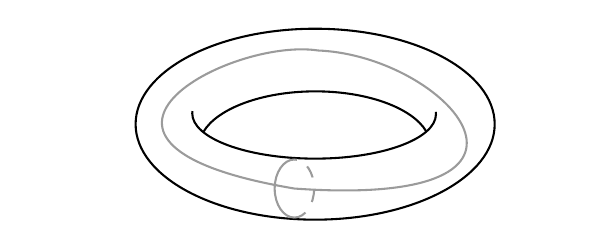
\begin{tikzpicture}[x=0.75pt,y=0.75pt,yscale=-1,xscale=1]
%uncomment if require: \path (0,300); %set diagram left start at 0, and has height of 300

%Shape: Ellipse [id:dp10888654123535657] 
\draw   (91,139) .. controls (91,113.59) and (129.73,93) .. (177.5,93) .. controls (225.27,93) and (264,113.59) .. (264,139) .. controls (264,164.41) and (225.27,185) .. (177.5,185) .. controls (129.73,185) and (91,164.41) .. (91,139) -- cycle ;
%Shape: Arc [id:dp9067895132467914] 
\draw  [draw opacity=0] (235.63,133.04) .. controls (235.69,133.42) and (235.71,133.81) .. (235.71,134.19) .. controls (235.67,146.12) and (209.35,155.7) .. (176.93,155.59) .. controls (144.5,155.48) and (118.25,145.73) .. (118.29,133.81) .. controls (118.29,133.42) and (118.32,133.05) .. (118.37,132.67) -- (177,134) -- cycle ; \draw   (235.63,133.04) .. controls (235.69,133.42) and (235.71,133.81) .. (235.71,134.19) .. controls (235.67,146.12) and (209.35,155.7) .. (176.93,155.59) .. controls (144.5,155.48) and (118.25,145.73) .. (118.29,133.81) .. controls (118.29,133.42) and (118.32,133.05) .. (118.37,132.67) ;
%Shape: Arc [id:dp7282595977083575] 
\draw  [draw opacity=0] (230.99,142.4) .. controls (224.37,131.23) and (202.8,123.1) .. (177.25,123.18) .. controls (151.77,123.27) and (130.31,131.5) .. (123.69,142.66) -- (177.34,149.79) -- cycle ; \draw   (230.99,142.4) .. controls (224.37,131.23) and (202.8,123.1) .. (177.25,123.18) .. controls (151.77,123.27) and (130.31,131.5) .. (123.69,142.66) ;

%Shape: Arc [id:dp4865327224674516] 
\draw  [draw opacity=0] (167.5,184) .. controls (167.5,184) and (167.5,184) .. (167.5,184) .. controls (162.25,184) and (158,177.73) .. (158,170) .. controls (158,162.27) and (162.25,156) .. (167.5,156) -- (167.5,170) -- cycle ; \draw  [color={rgb, 255:red, 155; green, 155; blue, 155 }  ,draw opacity=1 ] (167.5,184) .. controls (167.5,184) and (167.5,184) .. (167.5,184) .. controls (162.25,184) and (158,177.73) .. (158,170) .. controls (158,162.27) and (162.25,156) .. (167.5,156) ;
%Shape: Arc [id:dp049149640047466026] 
\draw  [draw opacity=0][dash pattern={on 4.5pt off 4.5pt}] (167.5,184) .. controls (167.5,184) and (167.5,184) .. (167.5,184) .. controls (172.75,184) and (177,177.73) .. (177,170) .. controls (177,162.27) and (172.75,156) .. (167.5,156) -- (167.5,170) -- cycle ; \draw  [color={rgb, 255:red, 155; green, 155; blue, 155 }  ,draw opacity=1 ][dash pattern={on 4.5pt off 4.5pt}] (167.5,184) .. controls (167.5,184) and (167.5,184) .. (167.5,184) .. controls (172.75,184) and (177,177.73) .. (177,170) .. controls (177,162.27) and (172.75,156) .. (167.5,156) ;

%Curve Lines [id:da7562826546508461] 
\draw [color={rgb, 255:red, 155; green, 155; blue, 155 }  ,draw opacity=1 ]   (179,103.5) .. controls (136.5,97) and (39.5,148.5) .. (167.5,170) .. controls (308,180) and (241,106) .. (179,103.5) -- cycle ;




\end{tikzpicture}
    }
    \caption{环面的拓扑性质}
\end{figure}

回忆一下,体系的希尔伯特空间维数为$2^{2N}$。当$2N-2$个边的自旋已经确定之后,系统的状态实际上已经确定了,因为约束条件\eqref{eq:toric-code-pair-condition}会确定剩下两条边的自旋。
换而言之,实际物理的希尔伯特空间维数只有$2^{2N-2}$。
这就意味着总希尔伯特空间$2^{2N}$分裂成了4支,或者说每个状态都有四重简并。
这个事实——环面上的Toric-code模型会出现基态四重简并——是\eqref{eq:toric-code-pair-condition}决定的,而\eqref{eq:toric-code-pair-condition}本身又来自环面的拓扑性质。
如果我们在哈密顿量中引入一个局部的扰动,基态能量和基态波函数显然会发生扰动,但是由于${A}$和${B}$的定义没有变化,系统拓扑没有变化,\eqref{eq:toric-code-pair-condition}也是始终成立的。
换句话说,环面上基态的四重简并是\concept{受到拓扑保护}的,局域的扰动不能让它消失。

用什么标记这四重简并?容易想到,完全可以定义一种全局性的闭弦算符,它贯穿整个环面,而由周期性边界条件它是闭弦算符。(这些算符的定义本身和拓扑紧密相关,显然如果系统被放在一个平面上那么根本没法定义全局性的闭弦算符)
分别沿着$x$轴和$y$轴定义
\begin{equation}
    {L}^x_\text{e} = \prod_{x} {\sigma}^z_{\vb*{i}}, \quad {L}^x_\text{m} = \prod_{x} {\sigma}^x_{\vb*{i}},
\end{equation}
并可以验证它们和哈密顿量是对易的,且它们构成一对对易稳定子。
这就意味着它们的本征值均为$\pm 1$,这就唯一地标记了四重简并。

以上两个弦算符标记的这种稳定的基态简并意味着Toric-code模型中显然有某种序,但这种序并不是使用对称性标记的,即和金斯堡-朗道理论中的那种局域的序是不同的。
的确,Toric-code中存在\concept{拓扑序}。

${L}^x_\text{e}$和${L}^x_\text{m}$将e粒子绕着$x$轴转动一圈,因此它们的本征值实际上给出了$x$方向类似于磁通量的一个通量,这个通量导致了一个Berry相位。

类似地还可以定义${L}^y_\text{e}$和${L}^y_\text{m}$,并且
\begin{equation}
    \acomm*{{L}^x_\text{e}}{{L}^y_\text{m}} = 0.
\end{equation}
我们知道
\begin{equation}
    \ket{0} = \ket{L_\text{e}^y=1, L_\text{m}^y=1},
\end{equation}
而使用这些关系可以证明,
\begin{equation}
    \begin{aligned}
        {L}^x_\text{e} \ket{0} &= \ket{L_\text{e}^y=1, L_\text{m}^y=-1}, \\
        {L}^x_\text{m} \ket{0} &= \ket{L_\text{e}^y=-1, L_\text{m}^y=1}, \\
        {L}^x_\text{m} {L}^x_\text{e} \ket{0} &= \ket{L_\text{e}^y=-1, L_\text{m}^y=-1}.
    \end{aligned}
\end{equation}
我们发现四重简并和四种基本的任意子正好能够对应上。这是拓扑序的一般特征:基态简并和任意子有对应,基态简并数目就是任意子数目的亏格次方。
我们这里是在亏格(洞的数目)为1的环面上工作,因此基态简并的数目为$4^1=4$种。
如果在亏格为0的球面上,基态简并的数目就是$4^0=1$种。
还有另一种方法也可以推导出这个结果。设亏格为$g$,由欧拉公式
\[
    V - E + F = 2 - 2g,
\]
于是
\[
    E - (V + F - 2) = 2g.
\]
而$V$是$A_s$格点的数目,$F$是$B_p$格点的数目,再减去\eqref{eq:toric-code-pair-condition}造成的两个约束,则$V+F-2$是一个二维表面Toric-code态的自由度个数。
Toric-code模型总的自由度个数为$E$,因此有$2g$个自由度用于标记简并态,由于每个自由度有两个取值,简并度为
\[
    2^{2g} = 4^g.
\]

我们看到,拓扑性质让基态简并出现,而基态简并意味着基态中可以有持续存在的弦——基态可以不是空无一物的!
这个看起来非常神奇——但是完全在预料之中——的性质让Toric-code模型成为一类允许出现弦网凝聚的模型中比较简单的一个。

\section{$\mathbb{Z}_2$规范理论}

Toric-code是一个严格可解模型;实际上,它的一些重要性质在哈密顿量形式更简单(但是不再严格可解)的所谓\concept{$\mathbb{Z}_2$规范理论}中也会体现出来。
历史上发生的事情其实是相反的:先有了$\mathbb{Z}_2$规范理论,然后再有了为了分析这一类的理论具有的性质而生造出来的Toric-code模型。

电动力学是一个$U(1)$规范理论,其中费米子场可以发生任意的局域相位转动,而与之配套的规范场——电磁场矢势——发生一个局域平移。
本文中我们不要$U(1)$这么大的对称性,而是只希望费米子场或者不发生相位转动,或者相位就转动$\pi$,在这样的规范对称性——也就是\concept{\Ztwo规范对称性}下系统的动力学保持不变。
如果我们还是在通常的四维时空中工作那么局域\Ztwo变换就是不连续的:因为$0$和$\pi$不能连续过渡。
因此我们将在格点上工作,即研究格点规范场论。

\subsection{$\mathbb{Z}_2$自旋液体的低能有效理论:费米型spinon和$\mathbb{Z}_2$规范场耦合}

\subsubsection{费米子的规范不变的跃迁项}

在二维格子上,格点上的费米子的动能项无非是从一个点跃迁到另外一个点,即
\begin{equation}
    {H}_0 = - \sum_{\vb*{i}, \vb*{j}, \alpha} t_{\vb*{i} \vb*{j}} {c}_{\vb*{i} \alpha}^\dagger {c}_{\vb*{j} \alpha}.
    \label{eq:hopping-hamiltonian}
\end{equation}
这个哈密顿量在局域\Ztwo变换下不是不变的。
现在我们将尝试把这个哈密顿量改造成\Ztwo规范理论。

显然,费米子可以携带\Ztwo群的表示:我们只需要让$e$的作用是什么都不变,而$2$的作用是将$c$变成$-c$即可。
在格点模型中规范联络应该放置在方块的边上而不是点上,为此,我们修改$t_{\vb*{i} \vb*{j}}$系数,使之成为规范联络,在\Ztwo变换下能够吸收掉费米子场带来的变化。
容易看到,只需要指定
\[
    {c}_{\vb*{i} \alpha} \longrightarrow \eta_{\vb*{i}} {c}_{\vb*{i} \alpha}, \quad t_{\vb*{i} \vb*{j}} \longrightarrow \eta_{\vb*{i}} \eta_{\vb*{j}} t_{\vb*{i} \vb*{j}},
\]
就能够让哈密顿量具有局域\Ztwo对称性。由于$t_{\vb*{i} \vb*{j}}$只是在正负两种状态之间切换,替代它的规范联络$\sigma_{\vb*{i} \vb*{j}} = \pm 1$,于是用哈密顿量
\[
    {H} = - \sum_{\vb*{i}, \vb*{j}, \alpha} t_{\vb*{i} \vb*{j}} \sigma_{\vb*{i} \vb*{j}} {c}_{\vb*{i} \alpha}^\dagger {c}_{\vb*{j} \alpha}
\]
做路径积分,分别以${c}, {c}^\dagger$和$\sigma_{\vb*{i} \vb*{j}}$为积分变量即可得到一个\Ztwo规范理论。

现在我们回到正则量子化框架中,$\sigma_{\vb*{i} \vb*{j}}$在每一个格点引入了$\pm 1$两个状态,从而我们可以把它当成一个自旋$1/2$的自旋算符%
\footnote{实际上,这个“自旋算符”未必来自某个体系的内禀旋转不变性。
更加数学的说法是,由于每个格点都有两个状态,我们可以在每个格点引入一个$2\times 2$的厄米矩阵
\[
    {\sigma} = \pmqty{1 & 0 \\ 0 & -1}
\]
作为规范场对应的算符,而这正是泡利矩阵中的${\sigma}^z$。后面引入${\sigma}^x$等算符的目的也只是用于翻转规范场的状态。
}%
,从而哈密顿量为
\begin{equation}
    {H} = - \sum_{\vb*{i}, \vb*{j}, \alpha} t_{\vb*{i} \vb*{j}} {\sigma}^z_{\vb*{i} \vb*{j}} {c}_{\vb*{i} \alpha}^\dagger {c}_{\vb*{j} \alpha}
    \label{eq:minimal-z2-couple}
\end{equation}
希尔伯特空间为费米子的态空间直积上每一点的自旋$1/2$空间。\Ztwo规范变换为
\begin{equation}
    {c}_{\vb*{i} \alpha} \longrightarrow \eta_{\vb*{i}} {c}_{\vb*{i} \alpha}, \quad {\sigma}_{\vb*{i} \vb*{j}}^z \longrightarrow \eta_{\vb*{i}} \eta_{\vb*{j}} {\sigma}_{\vb*{i} \vb*{j}}^z.
\end{equation}
特别的,如果\eqref{eq:hopping-hamiltonian}实际上是一个紧束缚模型,\eqref{eq:minimal-z2-couple}就成为
\begin{equation}
    {H} = - t \sum_{\pair{\vb*{i}, \vb*{j}}} {\sigma}^z_{\vb*{i} \vb*{j}} {c}_{\vb*{i} \alpha}^\dagger {c}_{\vb*{j} \alpha} + \text{h.c.}.
    \label{eq:tight-binding-z2}
\end{equation}
此时$\sigma_{\vb*{i} \vb*{j}}^z$实际上仅仅定义在方块的边上,即不需要对不相邻的点对$\pair{\vb*{i}, \vb*{j}}$也对应对应的$\sigma_{\vb*{i} \vb*{j}}^z$。

\subsubsection{$\mathbb{Z}_2$规范场自身的哈密顿量}

现在我们讨论\Ztwo规范场本身的哈密顿量,根据电动力学中的经验,这实际上就是将\eqref{eq:tight-binding-z2}中的费米子自由度积掉%
\footnote{
    这当然要求费米子是有能隙的,不过这其实没什么问题,如果\eqref{eq:tight-binding-z2}中的费米子无能隙,我们就把它和一个普通的有能隙的紧束缚模型加起来再积掉费米子即可。
    与电动力学相类比,积掉费米子无非就是将介质中费米子对电磁场的响应等效为介电常数和磁化率的修正。

    此外注意到,由于我们在正则量子化框架中工作,积掉费米子自由度后希尔伯特空间缩小,原本的希尔伯特空间中的纯态将对应一个混合态。
    但是实际上这无关紧要,因为我们只需要假装不知道费米子存在,分析\Ztwo规范场的态空间,最后计算配分函数即可,并不需要真的处理自旋系统的密度矩阵。}%
后得到的仅仅关于\Ztwo规范场(而没有任何物质场)的一个理论。
严格做积掉费米子的计算是非常不现实的,不过也不必要——正如电动力学中那样,只需要保证哈密顿量本身是\Ztwo规范不变的即可。
我们首先先分析\Ztwo规范变换如何写成算符形式,然后分析积掉费米子自由度之后的哈密顿量会是什么形式的。

只有$\sigma$的理论中的规范变换是
\begin{equation}
    {\sigma}_{\vb*{i} \vb*{j}}^z \longrightarrow \eta_{\vb*{i}} \eta_{\vb*{j}} {\sigma}_{\vb*{i} \vb*{j}}^z,
    \label{eq:pure-sigma-ztwo}
\end{equation}
也就是说对每一条边上的${\sigma}^z$本征态,规范变换或是不改变它,或是加一个负号。我们希望将\Ztwo规范变换写成算符的形式,为此注意到在自旋$1/2$中,算符${\sigma}^x$可以翻转${\sigma}^z$的本征态,且${\sigma}^x$是厄米算符,于是一条边上的规范场翻转就是
\[
    {\sigma}_{\vb*{i} \vb*{j}}^z \longrightarrow {\sigma}^x_{\vb*{i} \vb*{j}} {\sigma}_{\vb*{i} \vb*{j}}^z {\sigma}^x_{\vb*{i} \vb*{j}}.
\]
任何一个\Ztwo规范变换都可以拆解成一系列作用在格点上的规范变换相乘,而作用在格点$i$上的规范变换翻转和这个格点连接的四条边上的规范场,于是作用在格点$i$上的规范变换为
\begin{equation}
    {Q}_i = \prod_{\pair{\vb*{i}, \vb*{j}}} {\sigma}^x_{\vb*{i} \vb*{j}} = \prod_{\pair{\vb*{j}, \vb*{i}} \in +_{\vb*{i}}} {\sigma}^x_{\vb*{i} \vb*{j}}.
    \label{eq:z2-charge}
\end{equation}
我们知道实际的系统都是定义在时空上的,所以似乎没有什么阻止我们在时间维上也做规范变换。
实际上,\eqref{eq:z2-charge}确实只是空间上的规范变换,但是由于处理时间上的规范变换需要使用并不常用的离散路径积分形式,一般的研究均只研究空间上的规范变换。

于是规范不变量就是和所有${Q}_i$对易的算符。由于是低能有效理论,我们考虑最低阶的两个\Ztwo规范不变量,得到
\begin{equation}
    {H} = - K \sum_{\pair{\vb*{i}, \vb*{j}}} {\sigma}^x_{\vb*{i} \vb*{j}} - J \sum_{\vb*{I}} \prod_{\vb*{l} \in \Box_{\vb*{I}}} {\sigma}^z_{\vb*{l}}.
    \label{eq:z2-2d-hamiltonian}
\end{equation}
这就是只含有\Ztwo规范场的\emph{一个}理论(当然,实际上还有很多其它的\Ztwo规范理论,是取其它\Ztwo规范不变量得到的)。
这样spinon为费米子的\Ztwo自旋液体的低能有效理论就是
\begin{equation}
    {H} = - K \sum_{\pair{\vb*{i}, \vb*{j}}} {\sigma}^x_{\vb*{i} \vb*{j}} - J \sum_{\vb*{I}} \prod_{\vb*{l} \in \Box_{\vb*{I}}} {\sigma}^z_{\vb*{l}} - t \sum_{\pair{\vb*{i}, \vb*{j}}} \sigma^z_{\vb*{i} \vb*{j}} c^\dagger_{\vb*{i}} c_{\vb*{j}}.
    \label{eq:z2-spin-liquid-ising-gauge}
\end{equation}
注意哈密顿量\eqref{eq:z2-spin-liquid-ising-gauge}和\eqref{eq:z2-charge}\emph{不是}对易的。
物理地说这是因为\eqref{eq:z2-spin-liquid-ising-gauge}的第三项即费米子跃迁项的规范变换不仅仅关于$\sigma^z$也关于$c$,或者换一个角度,由于费米子此时携带\Ztwo规范荷,单个格点上的\Ztwo规范荷是不能守恒的。

关于为什么我们考虑了最低阶的两个\Ztwo规范不变量而不是别的(特别是,${\sigma}^x$是怎么被牵扯进来的),可以从两个角度考虑。
最显然的解释当然是,最低阶的\Ztwo规范不变量具有最好的局域性,因此是更有可能出现的。

不过,实际上更加站得住脚的一个解释来自\eqref{eq:z2-2d-hamiltonian}的路径积分表述。
\eqref{eq:z2-2d-hamiltonian}是格点模型,所以我们做一个\emph{离散时间路径积分}。
一个\Ztwo规范场自由度在路径积分中要加上一个虚时间指标,即$\{\sigma^z_{\vb*{i} \vb*{j}}(\tau)\}$。
现在考虑以下理论:
\begin{equation}
    Z = \sum_{\sigma^z} \exp(\sum_{\tau} (J_{xy} \sum_{\Box} \prod_{l \in \Box} \sigma_l^z(\tau)  ) ),
\end{equation}
由于没有$z$方向上的边上定义了$\sigma^z$自由度,我们可以直接沿用\eqref{eq:pure-sigma-ztwo}作为三维经典统计理论的\Ztwo规范变换。
三维经典统计理论的形式应该是
% TODO
现在我们看到,\eqref{eq:z2-2d-hamiltonian}实际上是已经做了一定的规范固定的理论:我们将所有时间方向上的边上的\Ztwo场都固定为1了。
因此,\eqref{eq:z2-2d-hamiltonian}中残留的规范冗余性只能是空间上的,相应的规范变换由\eqref{eq:z2-charge}给出。

\subsection{$\mathbb{Z}_2$规范理论的对偶理论}\label{sec:z2-dual-ising-model}

无论是\eqref{eq:tight-binding-z2}还是\eqref{eq:z2-2d-hamiltonian}都具有\Ztwo规范不变性,如果我们认为规范自由度不具有物理含义(它实际上有没有物理含义取决于我们关心的物理量是不是只涉及规范不变量),那么这两个哈密顿量就含有额外的自由度。
我们要设法把规范等价的构型全部映射到同一个构型上,而把规范不等价的构型映射到不同的构型上。
为此,我们将每个方块赋予一个格点坐标$I$,从而诸$\{i\}$和诸$\{I\}$形成对偶格点坐标。
设$\Box_I$为$I$号方块($I$标记了以所有的方块的中心为格点形成的新格子的格点坐标,称为\concept{对偶格子}),我们定义
\begin{equation}
    {\tau}^x_I = \prod_{l \in \Box_I} {\sigma}^z_l,
    \label{eq:def-tau}
\end{equation}
上标$x$看起来很奇怪,不过我们很快会发现其作用。这样\eqref{eq:z2-2d-hamiltonian}中的第二项就可以很容易地写出了。注意到$\tau^x_I$只有$\pm 1$两种取值,我们可以把它看成某个表象下的$x$方向泡利矩阵。
至于第一项,如果将${\sigma}_{\vb*{i} \vb*{j}}^x$作用在某个${\sigma}^z$表象下的基矢量上面,那么边$ij$上的$\sigma^z$反号,其余什么都不变,这就是说,设边$ij$由方格$I$和$J$共享,则由定义\eqref{eq:def-tau},$I$和$J$对应的$\tau^x$也反号,其余不变;
另一方面,将${\tau}^z_I {\tau}^z_J$作用在一个态上,则$I$和$J$对应的$\tau^x$均反号(同样依据泡利矩阵的性质,即$z$方向泡利矩阵可以翻转$x$方向泡利矩阵的本征态)。
两个算符的作用效果完全一样,所以实际上
\begin{equation}
    {\tau}^z_I {\tau}^z_J = {\sigma}^x_{\vb*{i} \vb*{j}},
\end{equation}
从而我们得到
\begin{equation}
    {H} = - K \sum_{\pair{I, J}} {\tau}^z_I {\tau}^z_J - J \sum_{I} {\tau}^x_I.
    \label{eq:z2-2d-tau-hamiltonian}
\end{equation}

现在没有规范冗余了——${\tau}^x_{I}$和${\tau}^z_I$都是规范不变量。
要看出自由度减少了多少,注意到二维格子中一个方块有四条边,每条边由两个方块分享,因此如果有$N$个方块(从而有$N$个格点),那么有$2N$条边。另一方面,只有$N$个方格。
因此如果只以${\tau}^z_I$为动力学自由度,则我们将希尔伯特空间的维数从$2^{2N}$降到了$2^N$。
丢自由度是正常的,因为在以上过程中我们抛弃了规范自由度,但是需要验证只以${\tau}^z_I$为动力学自由度是不是把一些并非规范自由度的自由度(它们没有出现在哈密顿量中)也抛弃了。
如果规范不等价的态给出不同的${\tau}^x_I$取值,我们就可以确定没有丢掉真正含有信息的自由度。
% TODO

在上述从$\sigma^z$到$\tau^x$的过程中我们丢失了一半的自由度,也就是说,有一半的自由度是可以随意指定的;指定这些自由度就是选取了一个规范;不过要注意,这不是说我们指定一半$\sigma^z$的值就是选取了一个规范,因为\eqref{eq:z2-2d-hamiltonian}中$\sigma^z$确定的波函数随着时间演化,$\sigma^z$会发生变化,这和规范选取需要满足的要求不符合——例如电动力学中如果选择$\div{\vb*{A}} = 0$,那么它不会在随后的时间演化中变得不是零。

\eqref{eq:z2-2d-tau-hamiltonian}正是横场伊辛模型。因此\eqref{eq:z2-2d-hamiltonian}也经常称为\concept{伊辛规范理论},因为它实际上就是横场伊辛模型换了一个形式。
横场伊辛模型是一个二维量子模型,其零温配分函数的精确形式对应一个三维经典统计模型,实际上这个三维经典统计模型就是一个各向异性的伊辛模型(在虚时间上的最近邻相互作用和空间方向上的最近邻相互作用不同)。
我们知道三维伊辛模型一定会出现相变,有一个顺磁相和一个铁磁相,这来自其普适类%
\footnote{
    虽然\eqref{eq:z2-2d-tau-hamiltonian}对应的经典统计模型是各向异性的,这并不改变其普适类,因为总是可以适当调节$\beta$的尺度让该经典统计模型变成各向同性的。
}%
,因此零温下横场伊辛模型——从而\Ztwo规范场——也会有一个相变,随着参数$K / J$的变化,从一个相切换到另一个相。

有一个看起来的佯谬:我们知道伊辛模型有一个全局\Ztwo对称性,可以将全部自旋翻转过来,得到一个不同的态,而与此同时哈密顿量保持不变。
实际上这个对称性在\Ztwo规范场中就是不存在的——等效的横场伊辛模型的相变破缺的就是这个对称性,由横场伊辛模型和\Ztwo规范场理论的等价性我们知道\Ztwo规范场理论也有一个相变,并且这个相变没有破缺任何对称性。
因此,在这里我们就已经知道了\Ztwo规范场有一个与对称性无关的相变了,它称为\concept{Ising*相变}。
和此相变有关的激发见\autoref{sec:z2-topo-excitation}。

Ising*相变的存在本身已经说明,去掉一个规范理论中的规范冗余性会导致一些局域的信息变成全局的,一些全局的信息变成局域的。
实际上,考虑到\Ztwo规范场和费米子的耦合是$\sigma^z c^\dagger c$形式的,而使用\eqref{eq:z2-2d-tau-hamiltonian}中出现的量不能局域地表示出$\sigma^z$,将\Ztwo规范场部分的规范冗余性去除必然导致\Ztwo规范场和费米子耦合部分出现非局域性。
这正是规范理论的作用:允许规范冗余性存在意味着原本非局域的理论现在是局域的了。在高能物理中这件事尤其重要——实际上粒子物理标准模型就是这么建立的(见\qftdoc)。

\subsection{低能自由度和拓扑序}

\subsubsection{任意子:规范荷和磁通量}\label{sec:gauge-charge-flux-z2}

在二维的电动力学中,设通过一个方格的磁通量为$\Phi$,则
\[
    \ee^{\ii \Phi} = \prod_{l \in \Box} t_{\vb*{i} \vb*{j}}.
\]
二维情况下一个区域内有磁通量是真的可以认为这里有一个粒子的,因为显然磁场在这个区域内有一个鼓包,因此量子化之后会得到粒子;至于这样的粒子是不是足够稳定(或者说,能够让“磁通量粒子”呈现为谐振子能级的哈密顿量和实际系统是不是足够接近)则又是另一回事。
在本文涉及的\Ztwo规范场中可以如法炮制地定义
\begin{equation}
    \ee^{\ii \Phi_I} = \prod_{l \in \Box_I} {\sigma}^z_{\vb*{i} \vb*{j}} = {\tau}^x_I,
\end{equation}
也即,我们用费米子在方块上转一圈发生的相位改变来定义磁通量。与$U(1)$的情况不同,\Ztwo规范场中磁通量只有$0$和$\pi$两种,因为四个$\sigma^z$相乘要么是$1$要么是$-1$。
现在我们看到了${\tau}^x$的另一重意义:它标记了一个方块上的磁通量。
与电磁场中的较为复杂的情况不同,\Ztwo规范场中的磁通量就是肉眼可见量子化的,而且只有两个状态。
注意到$\tau_I^x$取$1$时能量较低而取$-1$时能量较高,我们可以将某个方块的磁通量取$\pi$当成一种激发态,称为\concept{m激发},以体现它和磁通量的相似之处。
一个空间区域内有m激发等于是说存在一条围绕着该空间区域的$\sigma^z=-1$弦,实际上是一个涡旋(可以考虑一下电动力学中的磁通量是什么样的),也可以称它为\concept{vison激发}(Vortex-Ising-son,三个词根分别表示此类激发形如涡旋、和伊辛场有关、是元激发)。

另一个可以模仿电磁场引入的概念是\Ztwo规范荷,我们已经看到,\Ztwo规范变换对应的规范荷为\eqref{eq:z2-charge},这个量的取值只有$\pm 1$(因为是四个$\sigma^x$的乘积)。
由于\eqref{eq:z2-charge}守恒,我们有如下\Ztwo规范场的高斯定律:
\begin{equation}
    \prod_{\vb*{j} \in +} \sigma^x_{\vb*{i} \vb*{j}} = \text{\Ztwo -charge at $\vb*{i}$} = \const,
    \label{eq:gauss-z2}
\end{equation}
这个常数可以取$1$也可以取$-1$,但是没有时间演化。
这个额外的条件将希尔伯特空间划分成没有重叠的很多支,不同分支的\Ztwo规范荷分布不同。
虽然规范荷通常是通过规范场和物质场的耦合项引入的,在积掉物质场之后还是可以构造出规范荷的表达式,因为规范不变性的要求极大地限制了规范场荷物质场耦合的方式。
正如在电磁场中,即使我们积掉了物质场,麦克斯韦方程中还是会有一个电荷守恒方程
\[
    \pdv{\rho}{t} + \div{\vb*{j}} = 0
\]
一样——即使我们不知道电磁场实际上和一个物质场发生了耦合,我们还是可以将电荷当成电场线的某种特殊分布(源和汇),而以它们为某种激发。
同理,在\Ztwo规范场中,$Q_i$取$-1$意味着更高的能量(计算一下能量期望值就知道),那么我们可以认为某个点$i$处$Q_i=-1$意味着这里出现了某个激发,从而一个\Ztwo规范荷被放置在了这里,无论其背后的机制是什么,无论是不是真的有一个物质场和\Ztwo规范场发生了耦合。
我们称这种激发为\concept{e激发},以体现它和电荷的相似性。e激发是$\sigma^x$弦的末端。

实际上,从\Ztwo规范变换的定义可以发现,在规范变换下$\sigma^z$算符变号而$\sigma^x$算符不变号,又注意到e激发和m激发的定义,我们会发现,大体上有
\[
    \sigma^z \sim \ee^{\ii A}, \quad \sigma^x \sim \ee^{\ii E}.
\]
连接两个e激发的$\sigma^x$弦可以看成电场线;有许多可能的连接两个e激发的$\sigma^x$弦这件事对应于有多条电场线。注意,虽然一个经典电场经常被画成一族电场线,可是其中并没有良定义的\emph{单独一条}电场线;有两个确定的e激发的多体波函数(经典地看,其中应该有确定的电场)是多个$\sigma^x$弦构型的线性叠加这件事就是前述“经典电场中无良定义的单独一条电场线”这个事实的量子版本。$\sigma^z$为负的bond连接成的线(注意,不是$\sigma^z$弦,而是处处和$\sigma^z$弦垂直)可以看成磁感线。

\eqref{eq:gauss-z2}和麦克斯韦方程导出的电荷守恒方程有一个重要的区别,就是前者要求规范荷在每一点都守恒,而后者允许规范荷的流动。但这个区别实际上并没有什么物理意义。
麦克斯韦方程本身也不规定电荷应该如何流动(这是本构关系应该做的事情),因此,每一点的电荷密度算符和纯电磁场的哈密顿量也是对易的。
麦克斯韦方程中会出现电流密度单纯是因为这本质上是一个洛伦兹协变的理论,从而如果一个四维矢量的时间分量出现了,其空间分量也会出现。
类似的,协变密度泛函理论中用于标记系统基态的物理量不仅包括电子数密度也包括电子流密度。

\eqref{eq:z2-2d-hamiltonian}中没有引入任何真的携带\Ztwo规范荷的物质场,如果引入了,本节中的${H}$就只是\Ztwo规范场的哈密顿量而不是完整的哈密顿量了,此时\eqref{eq:gauss-z2}的第一个等号当然仍然成立,但是每个点上的\Ztwo规范荷就未必总是不变的了,虽然规范对称性要求规范荷总量保持不变;我们在\eqref{eq:z2-spin-liquid-ising-gauge}中看到的就是这种情况。
我们将\eqref{eq:z2-2d-hamiltonian}中没有动力学的规范荷称为\concept{测试规范荷},这个名称的意味是显然的;它相比有动力学的规范荷更容易处理,后者的哈密顿量在坐标表象下基本上不会是对角化的。

还有一个表面上的不同是,麦克斯韦方程中显式地给出了电荷密度和电流密度,而此处的\Ztwo规范场理论中似乎没有。
但这个其实只是记号的问题,电磁场的\emph{哈密顿量}中实际上也没有出现电荷密度和电流密度。
麦克斯韦方程中会有电荷密度和电流密度是因为当我们从电磁场哈密顿量数学地导出运动方程时我们发现$\vb*{E}$的散度和$\vb*{B}$的旋度减去电场的时间导数似乎分别是某个东西的密度和流,从而暗示了“规范荷就在这里”,正如我们发现\Ztwo规范场中似乎有某个守恒荷\eqref{eq:z2-charge}一样。

最后一个疑难是,从无物质场的电动力学的拉氏量推导出的麦克斯韦方程显式地指明了空间中不存在电荷(因为$\div{\vb*{E}} = 0$)。
然而这实际上是对“能量最低”的不同理解造成的:在没有有动力学的物质场的情况下,$\div{\vb*{E}}$没有时间演化,即是守恒量;如果我们固定各点的$\div{\vb*{E}}$不动,对电动力学的拉氏量做有约束的最小化,就能够得到有测试电荷的麦克斯韦方程组;另一方面,如果不施加任何约束,那么只能够得到没有任何电荷的麦克斯韦方程组。
这里的关键在于,由于没有物质场,测试电荷——如果有的话——是完全不会变动的,初始场构型中测试电荷是多少,不管做怎样的时间演化,它都保持不变。
因此,从一个有测试电荷的场构型出发,必须手动将“存在测试电荷”这一信息以约束的形式引入,才能够得到正确的时间演化方程,因为测试电荷分布不同的场构型彼此不可能从一个演化到另一个,而不施加约束地最小化作用量却是在假定测试电荷能够变动。
从正则量子化的角度看,各点上的测试电荷都是守恒的,测试电荷分布不同的态之间不可能通过时间演化连接,即希尔伯特空间根据测试电荷的分布被划分为了不同分支。
我们在研究\Ztwo规范场时没有遇到这个疑难,因为一直在使用正则量子化,哈密顿量,希尔伯特空间的语言。

有意\emph{不使用}一个特定的场引入e激发(例如,在电动力学中,电子场引入携带着电荷的电子)而是使用上面的方式,通过规范理论内部的场构型引入e激发是有好处的。
我们在二维平面内工作,所以(正如后面会看到的那样)很可能出现任意子。
如果我们使用一个费米场引入e激发,那分析一个e激发和其它任意子的交换相位时就不必要地产生了额外的复杂性,例如,两个e激发交换同时需要考虑\Ztwo规范场导致的交换相位和费米子的交换相位。
相反,我们采取一种反过来的观点:认为\Ztwo规范场自身的特殊构型已经产生了e激发,而\Ztwo规范场和费米子耦合的哈密顿量(如\eqref{eq:tight-binding-z2})的作用是“把e激发和费米子粘在一起”。%
\footnote{
    这个说法的合理性同样可以通过和电动力学相对比看出来。
    QED中量子化后的光子模式就只有两个,但是光子内线实际上可以理解成有三种光子模式,其中还有一个“有源无旋”的纵波“光子”模式,它对应静止电荷激发出的库伦场,正是它给出了库伦相互作用。
    这种模式不能在真空中远程传播,在没有源的时候无法传播,所以很自然,不可能出现在外线中。

    但是,如果我们要抽象地分析“电荷激发出的场会有什么性质”,那么还是要把这个有源无旋的模式找回来。
    此时哈密顿量中电荷和电磁场耦合的项无非就是将电荷和这个有源无旋的模式结合在一起。
}%
这样e激发是一个独立的单元,分析起来方便很多。e激发被粘到外界粒子上这个过程的一个直观的展示见\autoref{info:xy-topological-order}。

可以看到e激发和m激发的定义和Toric-code模型中的定义完全一样——实际上,这就是为什么Toric-code模型中的两种激发被命名为e激发和m激发。
相应的诸如弦算符、开弦、闭弦等的定义也和Toric-code模型中完全一样,e激发和m激发之间的交换相位也是一样的。

\Ztwo规范理论中的e激发是完全守恒的,没有任何时间演化:如果一开始某个格点上没有e激发,那么就是没有。
最为简单的情况当然是系统中没有任何e激发,即对所有$\vb*{i}$,施加约束
\begin{equation}
    Q_{\vb*{i}} = 1,
    \label{eq:no-charge-constraint-z2}
\end{equation}
或者等价地说,往哈密顿量中引入一个罚函数
\begin{equation}
    H = - g \sum_{\vb*{i}} Q_{\vb*{i}} , \quad g \gg 1,
    \label{eq:z2-charge-hamiltonian}
\end{equation}
这会让体系变成一个toric-code模型,其中e激发是一个能隙无限大的元激发。约束\eqref{eq:no-charge-constraint-z2}可以看成一个gauge sector,其基态为全体$\sigma^z_{\vb*{i} \vb*{j}}$有确定的值1,激发态只有m激发或者说vison。
我们也有其它的gauge sector。做一个局部的规范变换会改变弦的走向,但是不会更动e激发和m激发的位置。

上述事实意味着从拓扑序的角度看,无物质场耦合,$K=0$的\eqref{eq:z2-2d-hamiltonian}——所谓的\concept{Wegner模型}——实际上是非常病态的一个东西。
由于e激发完全没有出现在哈密顿量中,m激发分布相同的态全部是能量简并的,从而,何为能量本征态的合适标签——或者说我们要在哪一组表象下工作——实际上是不清楚的。
在Wegner模型中,如果我们在$\sigma^z$的本征态附近工作,那么态的规范不变性就没有了,然而此时我们仍然能够良定义m激发。一个$\sigma^z$的本征态是若干具有不同e激发分布的横跨多个gauge sector的态的叠加,其中观察不到清晰的e激发。
由于$\sigma^x$弦在态中是完全缺席的,此时的vison激发和普通的涡旋毫无区别:没有任何非平庸交换相位。
这样的一个模型似乎很难说有什么拓扑序,vison和二维经典XY模型中的涡旋或是一些磁体中的skyrmion没有什么本质区别。
然而,我们这里研究\Ztwo规范场是为了研究自旋液体的行为,因此讨论e激发仍然是必要的。
讨论e激发的一个用处如下:如果在纯\Ztwo规范场中引入两个e激发,发现系统能量正比于e激发间距,即e激发是禁闭的,那么\eqref{eq:z2-spin-liquid-ising-gauge}中的费米子——在自旋液体中就是spinon——也是禁闭的。
存在清晰可辨、分布确定的e激发的某个态中,$\sigma^z_{\vb*{i}}$不再是确定的了,于是实际上此时系统基态是一个弦网凝聚态,这样才能让$Q_{\vb*{i}}$有确定的值;在这样的态中仍然有确定的vison,因为它是Wegner模型的守恒量。
因此,此时体系的激发态中存在清晰可辨的e激发和m激发,从而有交换相位等等,即系统具有拓扑序。

可见,在引入e激发之后(或者等价地说,向哈密顿量中引入\eqref{eq:z2-charge-hamiltonian},但是让$g$很小,来制造量子涨落),我们就得到了拓扑序。
因此,与\autoref{info:xy-topological-order}类似,可以将使用$\sigma^z$的能量本征态定义的vison激发(可以说是\emph{经典Wegner模型中的vison})看成$\mathbb{Z}_2$拓扑序中的、使用弦网凝聚态定义的m激发的前体(因为我们有弦算符、连接在弦算符两端的“粒子”等结构,粒子的交换对应弦的交叉,可以引入非平庸相位)。
正如\autoref{info:xy-topological-order}通过向原本会产生被弦连接的点状粒子的XY模型引入强烈的量子涨落,能够得到演生规范场和拓扑序一样,此处我们通过引入$\sigma^x$项来引起量子涨落,让e激发变得重要,且e激发和m激发的弦的交叉引入非平庸相位,能够从原本平庸经典Wegner模型中的vison出发获得拓扑序。
当然,\autoref{info:xy-topological-order}中的拓扑序可以使用$\mathbb{Z}_2$规范理论充当有效理论,因为XY涡旋和\Ztwo规范理论的m激发绑定在一起,而这里讨论的从Wegner模型出发得到的拓扑序中,有效理论就是$\mathbb{Z}_2$规范理论本身而已。

使用\autoref{sec:branching-stringnet-model}中的语言说,\eqref{eq:z2-2d-hamiltonian}和\eqref{eq:z2-2d-tau-hamiltonian}都可以看成弦网模型。
看起来,\eqref{eq:z2-2d-hamiltonian}中的弦是$\sigma^x$弦,其第一项是弦张力项,第二项是弦动能项,而\eqref{eq:z2-2d-tau-hamiltonian}中的弦是$\tau^x$弦,其第二项是弦张力项而第一项是弦动能项。
以$\tau^x$弦为标准看待\eqref{eq:z2-2d-hamiltonian},会发现$\sum \sigma^x$项,也就是$\sigma^x$弦的弦张力项,实际上是$\tau^x$弦的弦动能项,而$\sum_\Box \prod \sigma^z$项,也就是$\sigma^x$弦的弦动能项,实际上是$\tau^x$弦的弦张力项,虽然看起来形式复杂。
不过,既然我们关注的是\Ztwo规范场中的\Ztwo磁通量,实际上\emph{不应该}将\eqref{eq:z2-2d-tau-hamiltonian}看成一个弦网模型,而是应该将它看成粒子模型:横场伊辛模型中,$\tau^z \tau^z$项可以视为m激发的跃迁项,因为它可以让一个m激发跃迁到临近的格点上。
% TODO:$\tau$实际上是磁单极子

\eqref{eq:z2-2d-hamiltonian}中的$\sum_\Box \prod \sigma^z$。
在Toric-code模型中十分幸运的是哈密顿量中的所有项彼此对易,并且哈密顿量在将$\sigma^x$和$\sigma^z$交换,格子和对偶格子交换的操作下保持不变,从而。% TODO

我们尚未讨论在引入横场项(或者说弦张力项)之后,定义e激发和m激发是否有意义。如果系统的低能自由度中实际上没有清晰可辨的这两种激发,那么引入这些概念毫无意义。
e激发的意义是规范荷(当然,是根据\Ztwo规范场构型而定义的,相当于电动力学中的纵波光子),m激发的意义是磁通量。
在规范理论中一种常见的让它们不属于低能激发的机制是\emph{禁闭}。
一个规范理论的禁闭相中,规范荷之间存在强烈的相互吸引,或者说连接规范荷的弦有非常强的弦张力,从而规范荷被强烈地束缚在一起;另一方面,规范场模式本身期望不大而量子涨落很大,从而系统的低能自由度中同样没有规范场模式。
因此如果\eqref{eq:z2-2d-hamiltonian}处在禁闭相,那么e激发和m激发都是没有意义的。

具体什么激发被禁闭什么被解禁闭当然由$J$和$K$调控。我们在\autoref{sec:z2-quantum-phase-transition}中分析\Ztwo规范场的量子相变。

\subsubsection{电场和磁场}

实际上\eqref{eq:z2-2d-hamiltonian}还能够写成\Ztwo“电场”和“磁场”的函数。

\subsubsection{Toric-code拓扑序}\label{sec:z2-topo-excitation}

有一点需要注意:虽然\eqref{eq:z2-2d-tau-hamiltonian}和\eqref{eq:z2-2d-hamiltonian}是对偶的,但在对称性、局域性等方面两者还是不一样的。就冗余性而言,\eqref{eq:z2-2d-hamiltonian}有\Ztwo规范对称性,但\eqref{eq:z2-2d-tau-hamiltonian}只有全局\Ztwo对称性;这两个模型实际上都是有冗余的,后者的冗余意味着什么我们马上可以看到。
同样,在\eqref{eq:z2-2d-hamiltonian}中显而易见的局域约束,在\eqref{eq:z2-2d-tau-hamiltonian}中也会以一种非常不平凡的形式呈现出来。

vison激发一定成对出现,通过分析\Ztwo规范场理论的希尔伯特空间可以直接确认这一点(我们在Toric-code模型中已经做过这件事了)。
这就是说,vison激发不能够使用局域的算符单个地产生。
表面上,与之对偶的横场伊辛模型\eqref{eq:z2-2d-tau-hamiltonian}可以有奇数个vison激发,因为可以将奇数个方块上的$\tau^x$设置为$-1$,但实际上这来自横场伊辛模型的全局\Ztwo冗余性。
将$K$调大,则$\tau^x$激发会越来越倾向出现,当出现得足够多时发生凝聚,此时就发生相变,从解禁闭相进入禁闭相。
因此\Ztwo规范场的解禁闭相中确实有一个序,这个序就体现在存在vison激发上,但是无法使用一个局域的序参量表示这个序。

总之,实际上\Ztwo规范场的确有一个量子相变,然而这个量子相变和没有对称性任何关系:其有序相中特有的低能自由度是一些非局域的弦算符两端的任意子,而不是任何局域的序参量。
\Ztwo规范场理论\eqref{eq:z2-2d-hamiltonian}有零温量子相变,牵涉其中的两个相分别是任意子禁闭相和解禁闭相。
从横场伊辛模型\eqref{eq:z2-2d-tau-hamiltonian}中可以看到m激发是有能隙的,同样可以说明e激发也是有能隙的。
e激发和m激发可能有吸引相互作用,使得它们聚合形成的激发无能隙,不过此时单独讨论e激发和m激发又变得没有意义了(与费米子类比,此时已经出现费米子配对了)。
因此,解禁闭相中存在有能隙的任意子,这些任意子的任意子表等和Toric-code模型完全一样。
于是这个\Ztwo拓扑序称为\concept{Toric-code拓扑序},因为它和toric-code模型的拓扑序是一样的。
此处“一样的”指的是阿贝尔拓扑序具有同样的任意子表和交换相位,即具有等价的张量范畴,并不代表其任意子动力学完全相同,不过任意子动力学在拓扑序研究中也不是非常重要(见\autoref{back:anyon-tensor-category})。
我们可以认为Toric-code模型中的拓扑序构成了一个普适类,而Toric-code模型作为一个严格可解模型即为这个普适类中的重整化群不动点。


\subsection{零温量子相变}\label{sec:z2-quantum-phase-transition}

\subsubsection{对偶理论\eqref{eq:z2-2d-tau-hamiltonian}的视角}

根据\Ztwo规范场和横场伊辛模型的对偶关系,\Ztwo规范场的确有一个零温量子相变。
三维伊辛模型具有一个顺磁相和一个铁磁相,由于铁磁序的形成需要更多相互作用,$J/K$超过某个点时会出现顺磁相,否则出现铁磁相。
映射回二维横场伊辛模型,顺磁相意味着对偶格子上的各个$\tau$基本指向$x$方向,即有确定的磁通量;铁磁相意味着对偶格子上的各个$\tau$基本指向$z$方向,且要么几乎都为$1$要么几乎都为$-1$,没有确定的磁通量。
当$J$相对$K$很大时,对偶理论\eqref{eq:z2-2d-tau-hamiltonian}处于顺磁相,此时的基态几乎就是每个$\sigma^z$都取$1$的态,此时直觉上看,费米子可以畅行无阻;而当$J$相对$K$很小时,对偶理论\eqref{eq:z2-2d-tau-hamiltonian}处于铁磁相,此时的基态不是$\sigma^z$的本征态,投影在$\sigma^z$上有正有负,那么费米子似乎会被“迷惑”住(回忆一下,$\sigma^z$实际上是跃迁矩阵元),不知道怎么走。
那么,我们可以合乎情理地猜测,三维伊辛模型的顺磁相对应着\Ztwo规范场模型的一个解禁闭相,在其中\Ztwo规范荷清晰可辨,而三维伊辛模型的铁磁相对应着\Ztwo规范场模型的一个禁闭相,在其中携带有\Ztwo规范荷的费米子不能够单个的自由移动。

这样的论证当然是不够的,所以下面做一些半定量的论证。考虑\eqref{eq:z2-2d-hamiltonian}的格点路径积分(即虚时间轴也是离散化的),也即它对应的三维模型,定义
\begin{equation}
    W(C) = \expval{\prod_C \sigma^z_l(\tau)},
\end{equation}
其中期望值内部的算符乘积称为\concept{Wilson环算符},$C$是一个在虚时间方向上有延展的环路。
容易看出$W(C)$给出了从某个虚时间点开始产生一对e激发,按照$C$指示的轨迹扩散,经过一段时间之后又湮灭的概率(在经典理论中这是良定义的,因为没有任何不确定关系;具体有没有手段可以用量子测量的标准方法测出这个概率则是另外一回事),随着$C$扩大它理所当然会衰减,如果随着$C$扩大它衰减得很快那么就说明e激发总是成对地被束缚在一起。
我们本来可以使用两点格林函数来表征e激发被束缚的强度的,但是由于两点格林函数不是规范不变的,任何两点格林函数都是零。
$W(C)$的衰减方式有两种典型的形式:一种是\concept{面积定律},即
\begin{equation}
    W(C) \sim \ee^{-A},
\end{equation}
其中$A$是$C$围成的面积,另一种是\concept{周长定律},即
\begin{equation}
    W(C) \sim \ee^{-L}.
\end{equation}
设$C$持续时间为$\tau$,则按照虚时间演化,应该有
\[
    W(C) \sim \ee^{-\tau \Delta E},
\]
其中$\Delta E$是两个e激发同时出现造成的能量上升。我们马上可以看出,由于
\[
    A \sim \tau R,
\]
其中$R$是两个e激发的距离,如果面积定律成立,必然有
\[
    \Delta E \sim R,
\]
这是典型的禁闭效应:两个e激发离得越远,能量越高,当能量高到一定程度时涨落会导致新的e激发产生,从而产生两对离得非常近的e激发。
另一方面,如果周长定律成立,则
\[
    \Delta E \sim 1 + \frac{R}{\tau},
\]
而由于粒子通常不会跑太远,可以认为$\Delta E$基本上是一个常数,因此没有禁闭效应。

那么,前述横场伊辛模型给出的两个相是不是分别对应面积定律和周长定律?
我们尝试将$W(C)$映射到横场伊辛模型中,并在二维平面上计算$W(C)$。这实际上是有问题的,因为在用$W(C)$的行为判断是否有禁闭时,要求在时空上做Wilson回路,但此处我们单纯是在空间上做Wilson回路。
在\Ztwo规范场理论中这不会造成什么问题,因为它对应一个二维横场伊辛模型,后者对应一个三维经典伊辛模型,于是就有时间和空间的等价性。
由于Wilson回路能够使用的大部分模型都具有类似的性质,使用二维平面上计算出的Wilson回路来判断是否禁闭不会有问题,否则需要寻找别的回路算符。
因为$C$围成的区域内部的$\sigma^z$会被乘两次,于是就给出$1$,于是
\[
    \prod_{l \in C} \sigma^z_l = \prod_{l \in D} \sigma^z_l,
\]
依照$\tau^x$的定义即得到
\begin{equation}
    W(C) = \expval{\prod_{I \in D} \tau^x_I(\tau)},
\end{equation}
其中$D$是$C$围成的区域。
由于只有两个相,可以在$J/K$很小或很大时分别做微扰论,由此得到的关于相的结构的信息在整个相内部都是成立的。
$J \gg K$的情况对应顺磁相,系统基态形如
\[
    \ket*{\text{ground}} = \ket*{\tau^x = \rightarrow \rightarrow \cdots \rightarrow} + \frac{K}{J} \sum_{i, j} \ket*{\tau^x = \rightarrow \cdots \leftarrow_i \cdots \leftarrow_j \cdots \rightarrow} + \cdots,
\]
其中$i$和$j$相邻。
上式看起来很奇怪,不过真的去算期望会发现翻转两个$\tau^x$比翻转一个能量更低。(翻转相邻的两个${\tau}^x$的话,${\tau}^z_I {\tau}^z_J$项的期望不为零)
如果格点$i$和$j$在$C$内部,那么它不会对期望值有什么贡献,因为$-1$平方还是$1$;格点$i$和$j$在$C$外部那肯定也不会有什么贡献。
唯一会让期望值偏离$1$的激发是$i, j$中一个在$C$内部一个在$C$外部,于是我们有
\[
    \expval{\prod_{I \in D} {\tau}^x_I} \sim 1 - \frac{K}{J} L(C).
\]
那么,合理的猜测是,在顺磁相中应该有周长定律成立,于是没有禁闭。
铁磁相的讨论是类似的。 % TODO
我们仅仅讨论了两个极限情况,没有得到完整的$\ee$指数,但是一般的情况计算起来是非常困难的,此处略去。

总之,铁磁相($J / K \ll 1$)对应禁闭的\Ztwo模型的状态,顺磁相则对应非禁闭的\Ztwo模型的状态。禁闭相中,vison激发和\Ztwo规范荷不再是有意义的低能自由度。
由于禁闭相的基态非常接近${\tau}^z$的本征态,在其上讨论${\tau}^x$的排列模式——也就是m激发——并没有意义,在其中m激发有很强的量子涨落,然而没有任何比较稳定的低能激发可以使用$\tau^x$标记。
因此,m激发或者说vison激发不是有意义的低能自由度。
e激发不会被量子涨落抹去,然而注意到$J=0$时
\[
    H = - K \sum_{\pair{\vb*{i}, \vb*{j}}} \sigma^x_{\vb*{i} \vb*{j}},
\]
现在设一条弦两端各有一个e激发,则弦上各点都有$\sigma^x = -1$,于是系统能量相比于基态能量的增量就是弦的长度乘以$K$,因此会有一个全局不衰减的力将两个e激发拉在一起,即携带\Ztwo规范荷的费米子无法单个地自由移动。
因此禁闭相中的“\Ztwo激发”——e激发和m激发——都没有意义,即在这里\Ztwo规范场的行为并不十分有趣。
反之,在$K=0$时,m激发没有量子涨落,且e激发之间没有相互作用,因此e激发和m激发都是能够存在的。
与通常的情况不同,在\Ztwo规范场模型中,顺磁相是非平凡的,铁磁相反而是平凡的。

\subsubsection{禁闭相的性质}

应注意vison激发被禁闭这件事并不意味着系统的低能能量本征态中真的没有vison激发,正如虽然夸克被禁闭了,但是显然有质子、中子这些粒子的地方就有夸克。
vison被禁闭意味着,含有\emph{清晰可辨的}vison的状态不会出现,但是低能能量本征态中有若干含有vison的态叠加在一起是非常正常的。
实际上就是这样:$K \gg J$时基态波函数在$\sigma^z$表象下的不少分支都含有vison,然而vison激发也的确是被禁闭的。
因此这里又有一个迷惑性的地方:\Ztwo解禁闭相的基态中\Ztwo磁通量是被\emph{排除}的,但是低能激发中确实有m激发;\Ztwo禁闭相的基态中确实是有(很多的)m激发的,但是低能激发中没有稳定存在的m激发。
因此,\Ztwo的禁闭相其实可以看成\emph{任意子凝聚}相,而解禁闭相则是\emph{弦网凝聚}相。

从禁闭相和解禁闭相均为有能隙相而它们的基本自由度完全不同这件事出发也可以看出零温量子相变的存在。


% 实际上,对$J=0$的二维\Ztwo规范场,通过适当选取规范还可以将它转化为一系列一维伊辛模型的组合。 
% 我们取规范

% 此时的禁闭相对应于顺磁相,因为伊辛模型中的${S}^z$就是磁通量。

% TODO:是否:vison带有整数自旋(由于只区分拓扑性质,可以认为vison不带自旋,因为带有自旋的vison可以分解成一个带有自旋的平凡的激发和一个不带有自旋的vison激发)

\section{二维平面上格点$U(1)$规范场论}

我们现在来分析平面上的$U(1)$格点规范场论的性质。与\Ztwo规范理论不同,规范群为李群的规范理论中,规范场的元激发一般是无能隙的——电动力学就是一个典型例子。
因此,如果一个自旋液体的演生规范场的规范群是李群,那么其行为和一般意义上的(有能隙)拓扑序会有一些不同之处。

在格点规范场中允许存在磁单极子;此时它称为\concept{紧致的规范场},因为规范群是紧致的。
实际上,电动力学在格点上的规范群并不是$U(1)$的,因为$0$和$2\pi$不等价。
